\documentclass[a4paper,12pt]{book}
%\usepackage[sorting=none]{biblatex}
%\usepackage{natbib}
%\bibliographystyle{plainnat}
\usepackage[utf8]{inputenc}
\usepackage{graphicx}
%\usepackage{mathtools}
\usepackage{float}
\usepackage{amsmath}
\usepackage{epstopdf}
\usepackage[section]{placeins}
\usepackage{rotating}
\usepackage{graphicx}
\usepackage{fancyhdr}
\usepackage{nomencl}
\usepackage{mathrsfs}
\makenomenclature
\renewcommand{\nomname}{List of Symbols}
%\newcommand{\changefont}{%
%	\fontsize{7}{9}\selectfont
%}
%\fancyhf{}
%\fancyhead[LE,RO]{\changefont \slshape \rightmark} %section
%\fancyhead[RE,LO]{\changefont \slshape \leftmark} %chapter
%\fancyfoot[C]{\changefont \thepage} %footer
\begin{document}


\author{Massimo Turola}
\title{Investigation of plenoptic imaging systems: a wave optics approach}
\date{January 2016}


\clearpage
%\frontmatter
\mainmatter
\pagestyle{fancyplain}
\rhead{}
\renewcommand{\headrulewidth}{0pt}
\begin{titlepage}
    \begin{center}
        \vspace*{1cm}
        \LARGE
        \textbf{Investigation of Plenoptic Imaging Systems: a Wave Optics Approach}
        
       % \vspace{0.5cm}
        %Thesis Subtitle
        \large
        \vspace{1cm}
        \Large
        \textbf{Massimo Turola}
       
        \vfill
        \large
        A thesis presented for the degree of\\
        Doctor of Philosophy
        
        \vspace{0.8cm}
        
        
\includegraphics[width=0.4\textwidth]{C:/Users/Massimo/Documents/Thesis/logo.png}
        \\
        \large
        School of Health Science\\
        City University London\\
        January 2016
        
    \end{center}
\end{titlepage}
\baselineskip 24pt
\thispagestyle{plain}
\begin{center}
	\Large
	\textbf{Investigation of Plenoptic Imaging Systems: a Wave Optics Approach}
	\vspace{0.4cm}
	\\
	\large
	\textbf{Massimo Turola}
	
	\vspace{0.9cm}
	\textbf{Abstract}
\end{center}

Conventional imaging devices only capture a part of the total information carried by the light. A new generation of imaging devices, plenoptic systems, use an array of micro lenses to codify the light coming from an object into a four dimensional function called the light field. The final image is then obtained after post processing computations on the light field. \\
 In this work plenoptic imaging devices are analysed using a wave optics approach. A platform to simulate light propagating under the Fresnel approximation in a generic optical system was developed in MATLAB. An optical system can be modelled as the composition of two basic operators: the free space propagation and the lens. The first one was implemented developing an original method derived from the angular spectrum of plane waves theory of propagation. The second was implemented using a phase mask. The code was developed to optimize the signal to noise ratio and the computational time.
 \\
Two different configurations of plenoptic imaging systems were simulated. The first is the plenoptic 1.0 configuration. The general theory of plenoptic 1.0 and the post processing algorithms presented in the literature were verified using the simulation platform. The effects of diffraction were also evaluated and an original refocusing method is presented. For the second configuration, plenoptic 2.0, a full study of the optical resolution has been made and a detailed analysis of the effects of diffraction is presented. The results achieved with the simulations have been used to design a working prototype of a plenoptic microscope.
\\
 This novel wave optics approach enables us to quantify for the first time in the literature the effects of diffraction on this class of devices. In plenoptic 1.0 diffraction is a source of noise due to the crosstalk between neighbouring lenslets. In plenoptic 2.0 systems the optical resolution is directly proportional to the magnification of the lenslet array. A small magnification leads to a high directional sampling but at the same time to a loss of optical resolution. The finite dimensions of the lenslets together with the wave nature of light produce a physical limit to the amount of information that can be achieved sampling the optical fields with those kind of devices.
\begin{titlepage}

        \vspace*{1cm}
%        \LARGE
%        \textbf{Investigation of Plenoptic Imaging Systems: a Wave Optics Approach}
%        
%       % \vspace{0.5cm}
%        %Thesis Subtitle
%        \large
%        \vspace{1cm}
%        \Large
%        \textbf{Massimo Turola}
    
   \vspace{5cm}
    \raggedright  
      The scientific man does not aim at an immediate result. He does not expect that his advanced ideas will be readily taken up. His work is like that of the planter, for the future. His duty is to lay the foundation for those who are to come, and point the way.\\
      \raggedleft
      Nikola Tesla
%        
%        \vspace{0.8cm}
%        
%        
\includegraphics[width=0.4\textwidth]{C:/Users/Massimo/Documents/Thesis/logo.png}
%        \\
%        \large
%        School of Health Science\\
%        City University London\\
%        January 2016
        
\end{titlepage}
\tableofcontents
\printnomenclature	
\listoffigures
\listoftables
\baselineskip 24pt 
%\mainmatter
%\pagestyle{fancyplain}
%\rhead{}
%\renewcommand{\headrulewidth}{0pt}
%to print the list of symbols type in the command prompt the command 
%makeindex Thesis.nlo -s nomencl.ist -o Thesis.nls
\chapter*{Introduction}
\markboth{\MakeUppercase{Introduction}}{}
\addcontentsline{toc}{chapter}{Introduction}
\label{intro}
The information contained in the light surrounding the environment we live in is captured by different living beings according to the structure and the nature of their visual systems. The human eye is a single lens imaging system whose retina is composed of different types of photosensitive cells \cite{hart1992adler}. Those are rods, cones and photosensitive ganglion cells. There are three types of cone cell, each one with its specific absorption bandwidth centred on a specific wavelength giving to the retina the capability to act as a an RGB coclour sensor. For this reasons cameras have always been designed to capture light in the same way the human eye works, a single lens with three colour pixels producing two dimensional images based on three colours \cite{wetzstein2011computational}. \\
This way of designing cameras produces a loss of information with respect to all the information included into the light reaching the imaging system.\\
 The reality we see and measure with the instruments and the senses we have is just a projection of a more complex reality and great part of the information carried by the electromagnetic field is lost. This situation is similar to the one described in Plato's Allegory of the cave where a group of people are being chained for all their life inside a cave and facing a blank wall on which shadows of different objects are projected. For them the shadows produced by the objects passing in front of the fire are the only reality they know since they are limited in their perception by their situation \cite{plato1945republic} . The same happens with human perception and with the camera that imitates the human visual system. All conventional imaging instruments are limited and the images they produce are projections of a more complex quantity containing all information that light carries. Even the most advanced imaging instrument will always produce data that are close to reality, but that does not reach it, both because of intrinsic properties of light, such as diffraction, and because they have been designed to collect only a small set of reality. 
 Adelson and Bergen \cite{adelson1991plenoptic} in 1991 proposed to describe the whole set of information contained in the light by defining the plenoptic function, a seven dimensional function describing intensity, direction and wavelength of rays propagating in space. According to Adelson and Bergen a conventional imaging device captures projections of this function. For example a photo is obtained by integrating along the directional variables of the function, obtaining a two dimensional intensity pattern of the object imaged losing information on its three dimensional structure. If the integration is performed also along wavelength the image will be in grayscale and the information about wavelength will be lost. \cite{adelson1992single,ng2006digital}.
\\
This work will describe a new set of instruments that are able to sample the plenoptic function and the post processing methods to access all the information it carries. The character of this thesis will be mostly computational, and numerical simulations will be used as an instrument to explore the potential and define the limitations of this class of instruments.
\\
 The idea that more information is carried by the light contained in a scene was first proposed by Leonardo da Vinci who described the volume containing the light as filled by a dense array of light rays, which he called \textit{radiant pyramids} \cite{adelson1991plenoptic}. The plenoptic function described by Adelson and Wang \cite{adelson1991plenoptic} is the formalization of this concept of \textit{radiant pyramids} adding to the directions and positions of the rays information on the wavelength. Once the extra information contained in the scene has been understood the problem is to find a method to measure it. \\
 The first work about capturing the plenoptic function was done by Frederic Yves in 1903 \cite{ives1903parallax} on his works on parallax panorama-grams and by Lippmann in 1908 \cite{gabriel1908photographie} who proposed an array of pinhole cameras. The key to capture the plenoptic function is to have multiple views of the object to image. This can be done by translating a single camera to different positions over a spherical or planar surface \cite{levoy1996light,taguchi2010axial,gortler1996lumigraph}, a method known as time sequential sampling, or by using an array of cameras \cite{wilburn2001light,yang2002real,nomura2007scene} known as multi-sensor sampling. Multi-sensor techniques give high performances in term of resolution but are extremely complicated and expensive, while time-sequential techniques suffer the loss of the capability to capture dynamic scenes \cite{wetzstein2011computational}. The solution between cost and resolution is given by single-shot plenoptic sampling techniques based on a space multiplexing of the plenoptic function \cite{wetzstein2011computational}, as proposed by Herbert Ives \cite{ives1930parallax} and Lippmann \cite{gabriel1908photographie}. This single-shot space multiplexing method produces an array of elemental images on the sensor and this introduces several trade-offs between spatial and directional resolution \cite{wetzstein2011computational,georgiev2006spatio} as well as optical resolution trade-offs \cite{turola2014wave}. Several families of devices have been developed.\\ This work will describe those that sample the plenoptic function using an array of micro lenses in front of the sensor as described by Adelson and Wang \cite{adelson1992single}, Ng \cite{ng2005light}, Ng \textit{et al.}\cite{ng2006digital}, Ueda \textit{et al.} \cite{ueda2008adaptive} and Georgiev and Lumsdaine \cite{georgiev2010focused}. In particular Ng \textit{et al.} developed the first generation of plenoptic imaging systems, known as plenoptic 1.0, then improved by Georgiev who modified them giving birth to the second generations, or plenoptic 2.0. These two classes of instruments will be treated in this work. Other methods to capture the plenoptic function are based on creating mask patterns that enable frequency domain multiplexing of the plenoptic function \cite{veeraraghavan2007dappled,lanman2008shield}, compressive imaging techniques \cite{marwah2013compressive} or exotic solutions such as a slit camera \cite{ji2015depth}. The resulting images obtained with all these different methods contains all the extra information contained in the plenoptic function, but they are codified. Therefore the final image is obtained after implementing post processing algorithms in order to decode this information. For this reason the process of capturing plenoptic images is also called computational photography \cite{wetzstein2011computational,nayar2006computational}.\\ 
Along with the image rendering several post processing features can be performed once the information captured is decoded. These features include digital refocus and changing the point of view \cite{ng2006digital}, estimating depth \cite{ji2015depth,wetzstein2011computational,georgiev2012multifocus,georgiev2006light} and super-resolution imaging \cite{bishop2009light,shroff2013image,georgiev2009superresolution,georgiev2015plenoptic}. \\
\subsection*{Summary of the Thesis and its Novel Contribution to the Field}
The purpose of this work is to analyse the optical performances of micro lens array based plenoptic imaging systems. When this project started all existing work on this kind of instrument had been done using a ray optics approach and to place order in a relatively new field not yet well documented and understood. This work uses a wave optics approach so as to study the behaviour of a plenoptic imaging system at its diffraction limit. This is the first work that quantifies the effects of diffraction on the quality of raw sensor images and rendered images, defining a new trade-off between spatio-angular resolution and optical resolution. Most of the applications of plenoptic imaging considered in the literature preceding this work regarded photography and imaging of macroscopic objects. When attention is moved to the microscopic world, diffraction effects become important. The first thing that was done was to develop a simulation platform for wave propagation in a generic optical system. Existing methods to implement free space propagation have been investigated and a variant of one of the existing methods has been proposed in order to make it more efficient. This work also defines a new empirical method to simulate light in any state of coherence based on the true physical nature of coherence and it has been shown to give realistic results. Once the simulation platform was properly tested it was used to simulate a plenoptic imaging system. Different parameters were changed in order to investigate their influence on the optical properties of the system. At the same time post processing algorithms to extract information from the raw sensor data were developed following the methods in the literature. Some innovative solutions have also been developed. Different configurations of plenoptic setups have been compared, with particular attention to the optical performances of plenoptic 2.0 imaging systems. The results from these studies were then used to build a plenoptic microscope prototype in the laboratory.
\\
In the first chapter an introduction of plenoptic imaging is given. A rigorous explanation of how the seven dimensional plenoptic function can be reduced to a four dimensional function called light field is given. A definition of the light field will be given and an explanation of how the light field carries information regarding the 3D structure of the scene is provided including how it is sampled by the two different configurations, plenoptic 1.0 and plenoptic 2.0. A rigorous theoretical description of both classes of plenoptic systems is given using geometrical optics, with particular attention to the post processing methods to decode the information in it. \\
The second chapter is a description of the simulation platform developed in MATLAB that implements wave propagation of light under the Fresnel approximation. It has been designed to be a versatile and modular platform composed of operators that act on an input optical field to give an output field. The first operator described is the free space propagation based on the Fresnel approximation. The scalar theory of diffraction will be treated from a theoretical point of view starting from Maxwell's equations to end with the expression of Fresnel diffraction integral. Different methods to implement Fresnel propagation will be analysed highlighting advantages and disadvantages of each one of them in terms of resolution, signal to noise ratio and computational effort. To optimize the trade-off between the signal to noise ratio and digital aliasing a new wave propagation method is developed in this work and will be presented in this chapter. Then the lens operator is described and used to show results of simulation of simple optical systems with the purpose of comparing the performances of the five different free space propagation operators. This chapter is concluded with an explanation of the method to simulate partially coherent light which was developed.
\\
The third chapter is a complete description of a plenoptic 1.0 system explaining how to design and run simulations and how the to implement existing post processing algorithms in MATLAB to render the final image from the raw sensor data. Digital refocus principles and methods will be described. An original method to estimate the depth of point sources will be also proposed. 
\\
Chapter four focusses on the simulations performed to define the optical properties of a plenoptic 2.0 system. The impulse response of the system will be calculated together with its modulation transfer function. A frequency analysis of the system will be presented, showing how the different parameters of the system influence the optical resolution of the final rendered image. The detailed optical analysis of a plenoptic system using a wave optics approach is one of the key novel contributions of this work to the field.
\\
Chapter five contains the description of the setup built in the laboratory to verify the conclusions achieved with the simulations. A full description of the system will be given, as well as a description of the protocol to follow to capture light field images. Results from this laboratory prototype will be presented.
\\


\chapter{Theory and Methods of Plenoptic Imaging}
\markboth{\MakeUppercase{Theory and Methods of Plenoptic Imaging}}{}
\label{chap:chapter1}
\section{Introduction}
\label{sec:intro1}
A camera is a device that captures light in a scene \cite{zhou2011computational}. The main constituents of a conventional camera are the detector and lens. The rays of light passing through the aperture of the lens are recorded on the sensor as a two dimensional irradiance map of the scene imaged. Therefore a traditional camera performs a limited sampling of the complete set of rays and in general of the amount of information contained in the scene \cite{nayar2006computational}. Finding methods to quantify, extract and process the full set of information contained in the light field is a comnplex problem. The space is filled with a dense array of light with various intensities \cite{adelson1991plenoptic}. From each point of the object imaged a cone of rays departs and fills the whole space while propagating. If a traditional camera is placed at a certain position from the object it will sample only the rays passing through its aperture. The set of information contained in this cone of rays will then be recorded on a two dimensional plane. This process of recording light coming from a three dimensional scene on a two dimensional plane causes loss of information. Following Adelson and Bergen \cite{adelson1991plenoptic} all the information carried by the light propagating into space can be described by a function, called the plenoptic function. Different parametrizations of the plenoptic function are possible. One of these is a four dimensional function called Light Field that will be discussed in more detail in the next sections. A new class of optical instruments, called computational cameras are also described; these are able to record and extract information from the light field. Computational cameras differ form a conventional camera in the way they sample the light coming from the object using a non conventional new optics that codifies the light that hits the detector. This coded information is then decoded by a computational stage, in order to extract an image \cite{nayar2006computational}. Schematics of the difference between a conventional and a computational camera can be found in figure \ref{fig:systems}
\begin{figure}[H]
	\centering
	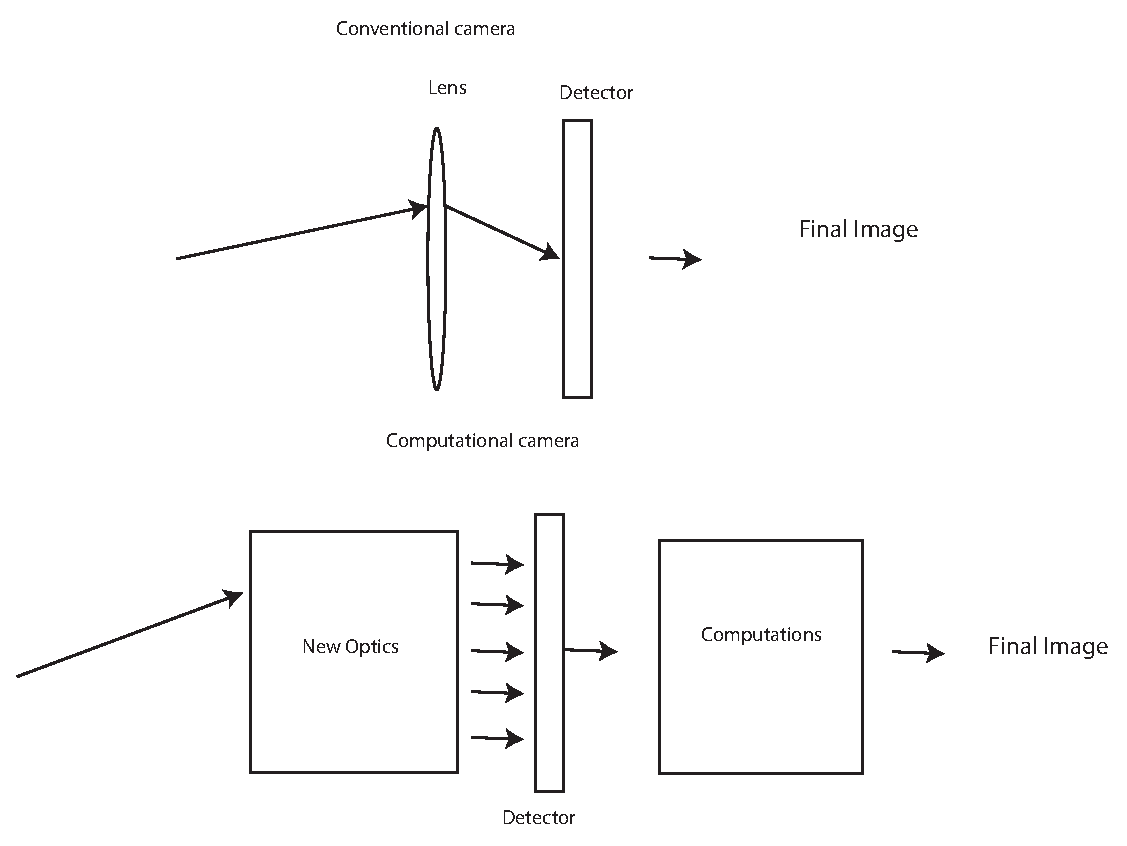
\includegraphics[width=.7\textwidth]{systemsNew.eps}
	\caption{\label{fig:systems}Differences between a traditional camera and a computational camera \cite{nayar2006computational}.}
\end{figure}
\section{Plenoptic Function and the Light Field}
\label{sec:lightfield}
A grayscale photograph taken by a conventional camera represents the intensity of light seen by a single viewpoint, at a single time, averaged and weighted over the wavelengths of the visible spectrum \cite{adelson1991plenoptic}. The term viewpoint is used to identify a direction of view of the scene. For each point of the sensor, the intensity can be represented as function of the position $P(x,y)$. A colour photograph adds information about the wavelength $\lambda$\nomenclature{$\lambda$}{Wavelength of the light} of the light adding a third variable, $P(x,y,\lambda)$. If several photos are taken in succession forming a movie the time dependence is added, $P(x,y,\lambda,t)$ and if the movie is captured using holographic techniques, i.e. saving phase and amplitude of the optical field, all the information regarding the light intensity observable form any viewpoint $\overrightarrow{V} = (V_x, V_y, V_z)$ is recorded. Therefore to describe all the information that is potentially available from the light coming from the object a seven dimensional function is needed. It takes the name of plenoptic function and its name comes from Latin \textit{plenum} that means full \cite{adelson1992single, adelson1991plenoptic,wetzstein2011computational}. The plenoptic function implicitly contains a description of every possible photograph that can be taken of a particular scene from any possible point of view. To record the plenoptic function, one should move the camera along all the possible positions $\overrightarrow{X}=(x, y, z)$ around the object and take a snapshot or have an array of cameras surrounding the object taking snapshots simultaneously. The plenoptic function is an idealized concept and it is impossible to record it completely. However it is possible to acquire samples of it or projections along one or more dimensions. For example a conventional grayscale picture is a two dimensional slice along the coordinates x and y of the seven dimensional plenoptic function taken from a single point of view, averaging the wavelength and integrating over the exposure time. A plenoptic camera is able to record a section of the plenoptic function \cite{adelson1991plenoptic}. In particular, it records the part of the plenoptic function whose rays pass through the aperture of the camera, hence all the possible viewpoints contained in the lens aperture. Final images are constructed by sectioning the plenoptic function along certain coordinates. The process of extracting information from the plenoptic function is called rendering \cite{levoy1996light,georgiev2010focused} and it is where the computational stage operates. 
Before proceeding in describing a plenoptic camera in detail it is useful to define another parametrization of the plenoptic function derived by Levoy and Hanrahan \cite{levoy1996light} that is more useful to implement the computational algorithms in the following sections. This parametrization is called light field and is the radiance as a function of position and direction \cite{levoy1996light}. It is described by a set of four coordinates, two spatial coordinates and two directional coordinates and for this reason is often referred to as the 4D Light Field. There are two possible representations of the light field: the two-point representation and the point-angle representation. With reference to figure \ref{fig:lightfield} in the two point parametrization a ray of light is propagating in the free space from the point \textit{(x,y)} to the point\textit{ (u,v)}. Its direction of propagation in the three dimensional space is defined by the two points where it crosses two parallel planes. Therefore the set of coordinates \textit{(x,y)} and \textit{(u,v)} defines only one ray of light \cite{levoy1996light}. The point angle parametrization instead uses the coordinates of the point where the ray intercepts a plane perpendicular to the optical axis, and the angles that it forms with the optical axis along the directions x and y, namely $\theta_x$ \nomenclature{$\theta$}{Angular coordinate} and $\theta_y$, as shown in figure \ref{fig:lightfield2} \cite{georgiev2006light}. In both cases the intensity is a function of four coordinates. \\ The 4D light field is therefore:
\begin{equation}
\label{eq:lightfield}
L(x,y,u,v) = L(x,y,\theta_x,\theta_y)
\end{equation}
\begin{figure}[H]
	\centering
	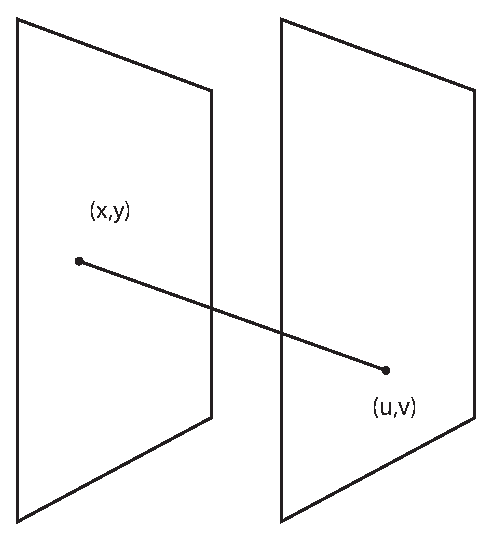
\includegraphics[width=.3\textwidth]{C:/Users/Massimo/Documents/Thesis/Thesis_PhD/lightfield.eps}
	\caption{\label{fig:lightfield}Two point representation of the light field. Each ray of light is uniquely defined by the coordinates of two points of interception.}
\end{figure}
\begin{figure}[H]
	\centering
	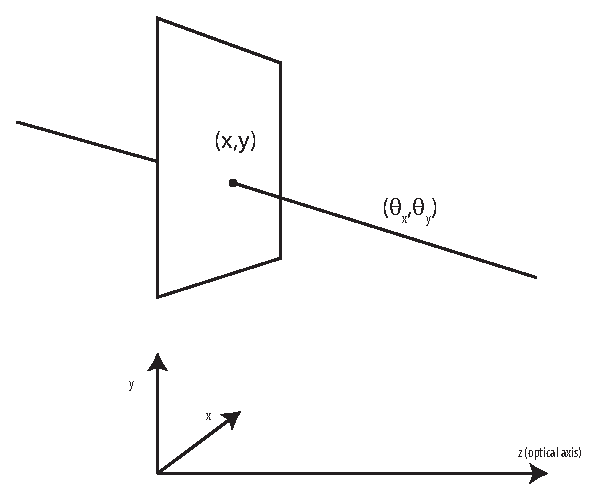
\includegraphics[width=.6\textwidth]{C:/Users/Massimo/Documents/Thesis/Thesis_PhD/lightfield2.eps}
	\caption{\label{fig:lightfield2}Point angle representation of the light field. A ray of light is uniquely defined by the coordinates of a point that belongs to a plane perpendicular at the optical axis z and by the angles $\theta_x$ and $\theta_y$ that it forms with the optical axis along the directions x and y.}
\end{figure}
For each pixel of the sensor of a plenoptic camera it is possible to determine these four coordinates. The information provided by the two extra directional coordinates enables a set of computational features such as 3D reconstruction, synthetic refocus, full depth of field and aberration correction \cite{ng2006digital}. Each of these features is possible after having decoded the light field with the computational stage as shown in figure \ref{fig:systems}.
\section{Plenoptic Camera}
\label{sec:plenoticcamera}
A plenoptic camera is a camera that records the 4D light field as described in equation \ref{eq:lightfield}. The version proposed and built by Adelson and Wang in 1992 \cite{adelson1992single} is composed of a main lens, a sensor and a micro lens array placed in front of the sensor \cite{adelson1992single}. The presence of the micro array enables the codification of the directional information on the sensor, as will be discussed in the next sections. This coded image represents the raw data of the plenoptic camera and it can be seen in figure \ref{fig:plenoptic1}: 
\begin{figure}[H]
	\centering
	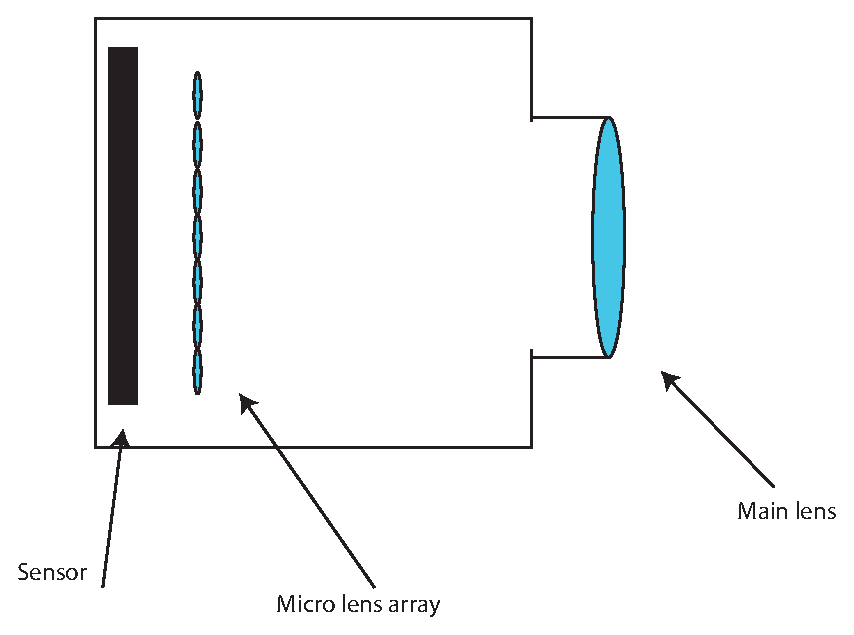
\includegraphics[width=.6\textwidth]{C:/Users/Massimo/Documents/Thesis/Thesis_PhD/plenopticamera.eps}
	\caption{\label{fig:plenoptic1} Plenoptic camera and its fundamental components. The presence of the micro array allows to record the light field .}
\end{figure}
The optical performance of the camera depends on the array's design characteristic. The main issue with the micro lens array is its position with respect to the main lens and the sensor. Depending on where it is placed two types of cameras are possible:
\begin{itemize}
	\item if the main lens forms its image on the micro array and the sensor plane is conjugated with the main lens it is the first generation plenoptic camera, or plenoptic 1.0 \cite{ng2005light} as seen in figure \ref{fig:plenoptic2} top.
	\item if the main lens forms its image on a plane that is different from the micro array plane and the micro lenses image the main lens image plane on the sensor it is the focused plenoptic camera, or plenoptic 2.0 \cite{georgiev2010focused} as seen in figure \ref{fig:plenoptic2} bottom.
\end{itemize}
 In the next sections both configurations will be extensively analysed and the way in which they capture the light field will be explained with particular attention to the differences in the raw data they produce. Their performances in term of lateral and directional (or angular) resolution will be detailed. The computational algorithms to render images from the raw data will also be extensively explained.
\begin{figure}[H]
	\centering
	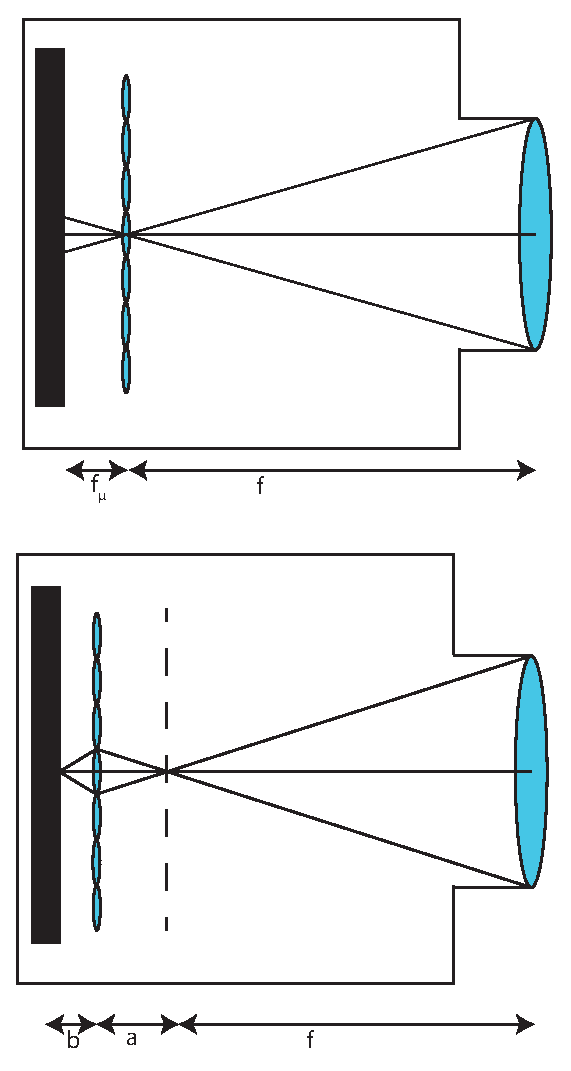
\includegraphics[width=.4\textwidth]{C:/Users/Massimo/Documents/Thesis/Thesis_PhD/plenoptic10.eps}
	\caption{\label{fig:plenoptic2}Top: Plenoptic camera 1.0. The main lens is focused on the object and forms an image on the micro array. $f$ is the focal length of the main lens and $f_\mu$ the focal length of the micro lens array. Bottom: Plenoptic camera 2.0. The main lens is focused on an object and forms an image on the plane represented by the dashed line. The micro array acts as a relay between the main lens image and the sensor, satisfying the lens equation $1/a+1/b=1/f_\mu$.}
\end{figure}
\section{Plenoptic Camera 1.0}
\label{sec:camera10}
The first version of the plenoptic camera has been proposed and realised by Adelson and Wang in 1992 \cite{adelson1992single} and then improved by Ng $et al.$ \cite{ng2005light} and by Ng \cite{ng2006digital}in 2005-6.\\ The purpose of Ng was to design a camera that can use ray tracing techniques to compute synthetic photographs after the acquisition of the four dimensional light field. The main difference between Ng's camera and Adelson and Wang's camera is that the latter was a prototype that utilized a system of relay lenses from the main lens image plane and the micro lens array \cite{ng2005light} while in Ng's camera the array of micro lenses is placed directly in front of the sensor. Each micro lens forms an elemental sub image on the sensor and the directional information is contained inside the sub images. The main lens focuses the rays coming from one point on the object plane on a single point in the image plane. If an array of micro lenses is placed at this image plane all the rays will end up on a single micro lens. The micro lens will then split this bundle of rays on the sub image underneath it, separating the rays according to their direction. This is explained in figure \ref{fig:plenoptic3} where the plenoptic camera is modelled as a simple 2 f system. This behaviour can be achieved also using an array of pinholes instead as proposed originally by Yves. The problem using pinholes is that the amount of light reaching the sensor is considerably lower since a pinhole is restricting the energy output. Since the sensor plane is conjugate with the main lens under each micro lens there will be an image of the main lens aperture. For simplicity in figure \ref{fig:plenoptic3} the system is composed of only five micro lenses and each sub image is composed of only three pixels. The rays departing from a single point in the object plane shown in blue, red and green, are transferred by the main lens on a single micro lens. As an effect of the micro lens, each ray ends on a different pixel of the micro image.
\begin{figure}[H]
\centering
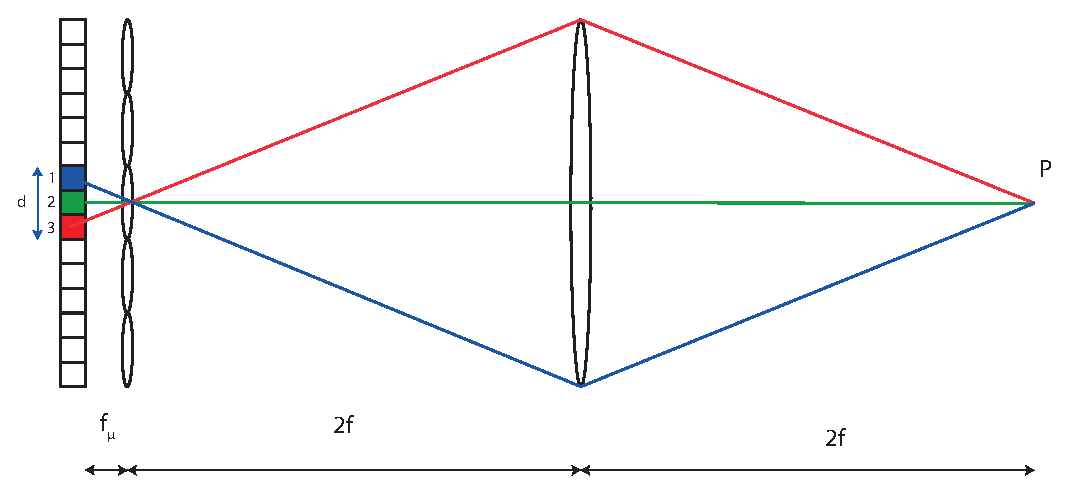
\includegraphics[width=.9\textwidth]{C:/Users/Massimo/Documents/Thesis/Thesis_PhD/raypleno10.eps}
\caption{\label{fig:plenoptic3}Ray diagram of a plenoptic 1.0 system. The main lens is in a 2f configuration and the sensor plane is conjugated with the main lens plane. The micro lens position maps the position (x,y) of the point P, while the sub image maps the directions of the rays coming from that point. The ray with direction $\theta_1$ falls on the pixel 1 (blue), the ray with direction $\theta_2$ falls on the pixel 2 (green) and the ray with direction $\theta_3$ falls on the pixel 3 (red). The sub image $d$ maps the direction of the rays.  }
\end{figure}
Since in the simplified case of figure \ref{fig:plenoptic3} there are only three pixels per micro lens, the maximum number of directions that can be sampled is three. A plenoptic camera samples as many directions as the number of pixels under each lenslet, therefore the directional resolution is given by the sub image resolution. Figure \ref{fig:plenoptic3} also shows that the spatial position of the point P is recorded at the micro array plane and the sampling of the position is linked to the number of lenses in the micro array. This leads to a trade-off between directional and spatial resolution since due to the finite dimension of the sensor, when more pixels are used to record the direction the same amount of pixels are lost to record the position. \\
With reference to figure \ref{fig:plenoptic4} two points are shown at two different positions on the same focal plane. The task now is to find a link between Levoy's and Hanrahan's two point representation of Light Field \cite{levoy1996light,levoy2006microscope} and the output data of the plenoptic 1.0 camera. Each sub image under each lenslet is an image of the main lens aperture, while the main lens image is formed on the micro array plane. To define the direction of a ray two points are needed. One point is its origin, the second is where it crosses the main lens. These two points are sampled by the lenslet array and by the sub images on the sensor, as shown in figure \ref{fig:plenoptic4}. Therefore it is possible to refer to the micro lens position on the array with spatial coordinates (x,y), and to the pixels of the sub images as the directional coordinates (u,v). With an array of 5 $\times$ 5 micro lenses and a sensor of 15 $\times$ 15 pixel, the 4D light field recorded will be a 5 $\times$ 5 $\times$ 3 $\times$ 3 function. Each point of this function is an intensity value identified by four coordinates, 2 spatial and 2 directional. the sampling of the spatial coordinates is 5 $\times$ 5, the sampling of the directional coordinates is 3 $\times$ 3. 
\begin{figure}[H]
	\centering
	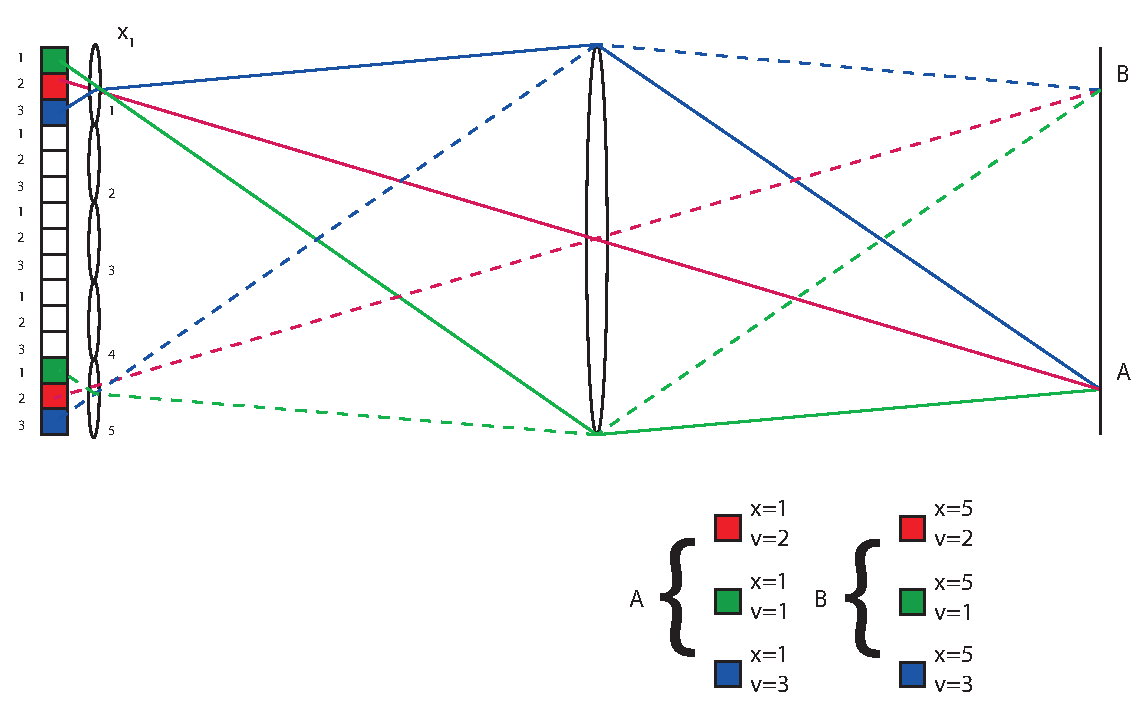
\includegraphics[width=.7\textwidth]{C:/Users/Massimo/Documents/Thesis/Thesis_PhD/plenoray2.eps}
	\caption{\label{fig:plenoptic4} Sampling of Light Field. Each ray is described by a set of four coordinates, two spatial (x,y) and two directional (u,v). The spatial coordinates are sampled by the position of the lenslet in the micro array, the directional coordinates are sampled by the pixel under the lenslet.}
\end{figure}
This sampling used in the example above is of course very low. The amount of light captured by a lens is defined by its f-number that is the ratio between the focal length and the aperture diameter. The f-number is proportional to the number of rays with different directions that enter into the main lens aperture diameter. The relative f-number can also be defined as the ratio of the distance between the lens and its image and the aperture diameter. 
\begin{equation}
\label{eq:f_num}
f_{\#} = \dfrac{v}{d}
\end{equation} 
where $v$ is the distance from the main lens and the image plane and $d$ its aperture diameter. Another useful quantity to describe the amount of directions sampled by a lens is its numerical aperture, defined, referring to figure \ref{fig:plenoptic5} as:
\begin{equation}
\label{eq:NA}
NA=n sin(\theta)\simeq n \theta =\dfrac{2}{f_{\#}}
\end{equation}
Where $n$ is the index of refraction, and $\theta$ is half the total range of directions sampled by the lens. The assumption of dealing with small angles was made because the distance from $u$ between the main lens and the micro array is bigger than the diameter of the micro lens. In air, n=1, therefore the relation between the f-number and the range of directions is given by:
\begin{equation}
\label{eq:fnum1}
\Delta\theta= 2\theta=\dfrac{4}{f_{\#}}
\end{equation}
 To be sure that all the directions sampled by the main lens are mapped into the light field, the f-number of the lenslet should match the f-number of the main lens \cite{ng2005light} as shown in figure \ref{fig:plenoptic5}. This condition known as f-number matching is very important in plenoptic imaging. If the f-number of the lenslet is smaller than the one of the main lens then there is an under sampling of the rays intercepted by the main aperture, since some of the pixels remain dark. If the f-number of the lenslet is bigger there is cross-talk between the sub images. In both cases directional information is in part lost (figure \ref{fig:plenoptic7}) .
\begin{figure}[H]
	\centering
	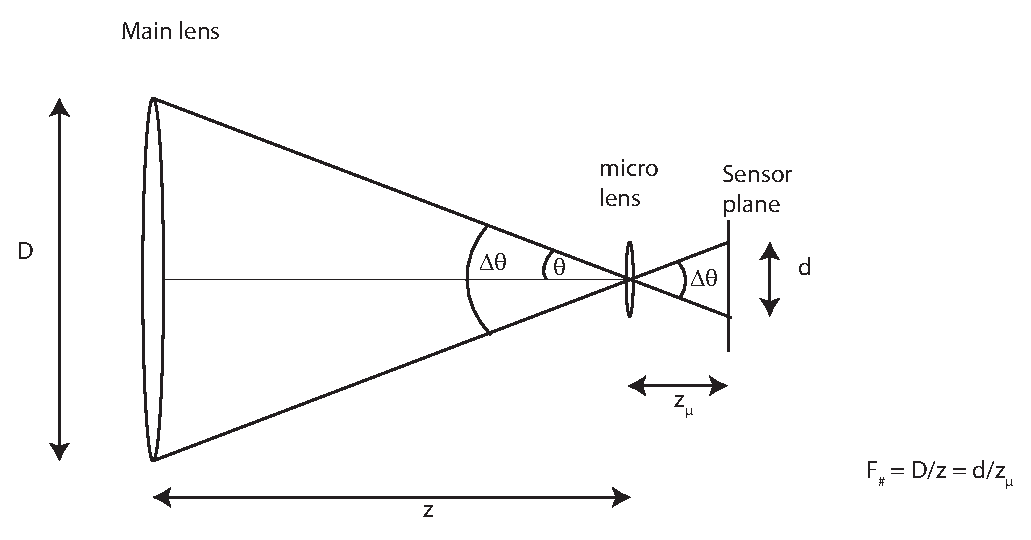
\includegraphics[width=.7\textwidth]{C:/Users/Massimo/Documents/Thesis/Thesis_PhD/fnumbermatching.eps}
	\caption{\label{fig:plenoptic5}F-number matching between the main lens and the micro lens in the array.  }
\end{figure}
\begin{figure}[H]
	\centering
	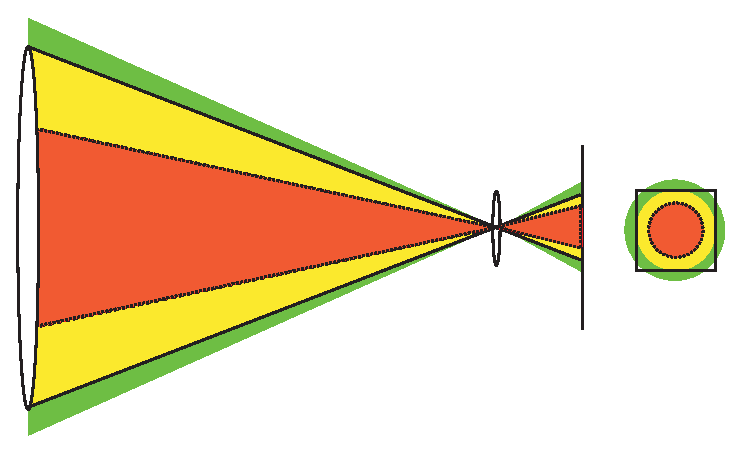
\includegraphics[width=.7\textwidth]{C:/Users/Massimo/Documents/Thesis/Thesis_PhD/fnumber2.eps}
	\caption{\label{fig:plenoptic7}When the f-number is matched, all the rays captured by the main lens are mapped on the sub image (yellow). If the f-number of the lenslet is smaller (red), the sub image is smaller and there is an under sampling of the set of rays. If the f-number of the lenslet is bigger (green), the sub image is larger and cross talk happens between neighbouring sub images .  }
\end{figure}
\newpage
\subsection{Phase Space in Plenoptic 1.0}
\label{sec:phase_space}
It is useful to analyse the sampling of the light field from a phase space point of view. In figure \ref{fig:plenoptic6} a point source is sampled by the lenslet array.\\
 The one dimensional case is considered here for simplicity. The single ray departing from the point P on the focal plane of the main lens is refracted by the optical system and is captured by a pixel on the sensor that belongs to the sub image of a lenslet. The sub image position on the array gives the coordinate x. The pixel of the sub image gives the direction $\theta_x$. Therefore in the phase space a single ray is represented by a point with coordinates (x, $\theta_x$).
Considering all the rays departing from the point \textit{P(x)} captured by the main lens, they will all be focused on a single lenslet and then split on the sub image. Each pixel of the sub image corresponds to a different direction (ray). In the phase space this is equivalent to a vertical line. The physical meaning is that for a single spatial position \textit{x} corresponds a range of $\Delta \theta_x$ possible different directions, defined by the numerical aperture of the main lens matched with the one of the lenslet.\\
\newpage
\begin{figure}[H]
	\centering
	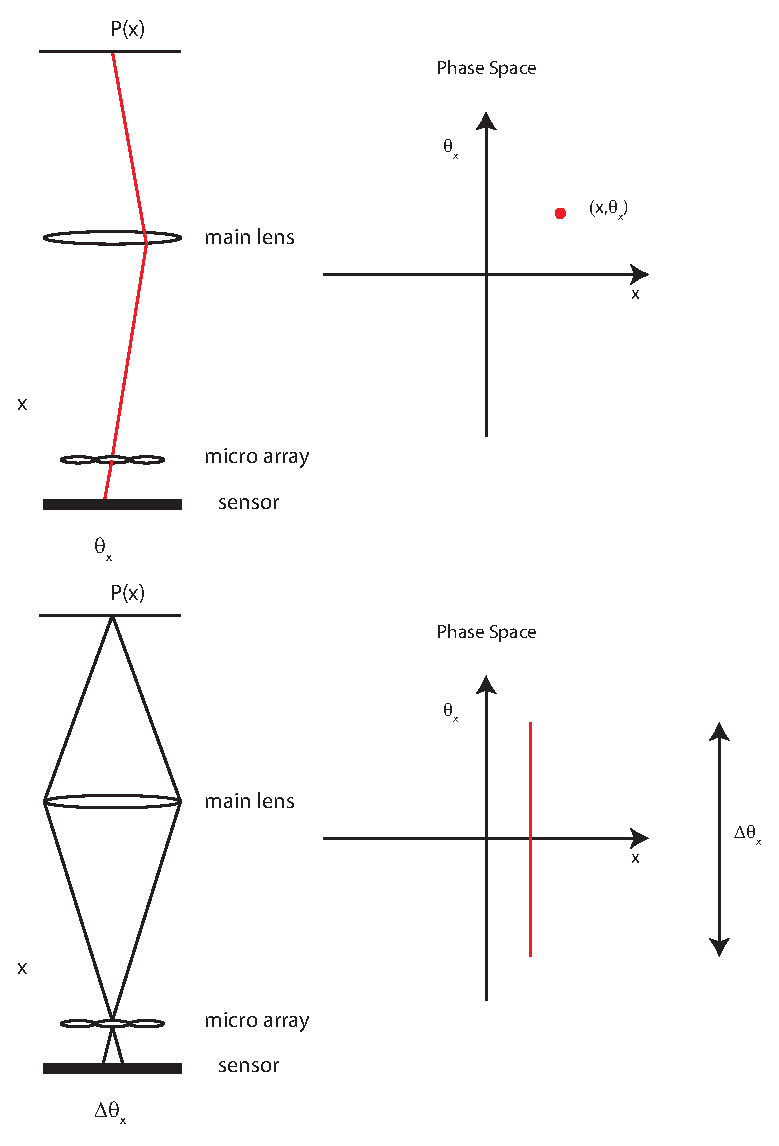
\includegraphics[width=.9\textwidth]{C:/Users/Massimo/Documents/Thesis/Thesis_PhD/phasespace10.eps}
	\caption{\label{fig:plenoptic6}Sampling of the light field and phase space representations of the rays.  }
\end{figure}
\newpage
\subsection{Light Field Parameterization}
\label{sec:LFparam}
Before discussing the rendering procedures for plenoptic 1.0 light field data, the three different parametrizations of the light field from the raw image will be described. A plenoptic 1.0 raw image looks like an array of sub images, each sub image contains samples of direction. An example of a plenoptic raw image can be seen in figure \ref{fig:rawlena10}. The raw image has been generated by simulating light propagating into a plenoptic camera, using a Matlab toolbox developed as part of this work which is described in detail in chapter \ref{chap:fresnel}. The simulated camera is composed of a 60 mm focal length lens, with an aperture of 7 mm, and a sensor with a resolution of 1500 $\times$ 1500 pixels. The micro array is composed of 75 $\times$ 75 lenslet with a focal length of 5 mm. The object imaged is a flat two dimensional image, therefore no depth information is stored. The reason for using flat objects to test a plenoptic imaging system is due to the fact that at this point of the work the interest is focussed on  understanding how the directions of the ray of light are recorded on the sensor, therefore reducing the degree of freedom of the problem to a flat isotropic isotropically emitting object simplifies the understanding of the problem. In the next chapters more accurate simulations will be presented taking into account the depth.
\begin{figure}[H]
	\centering
	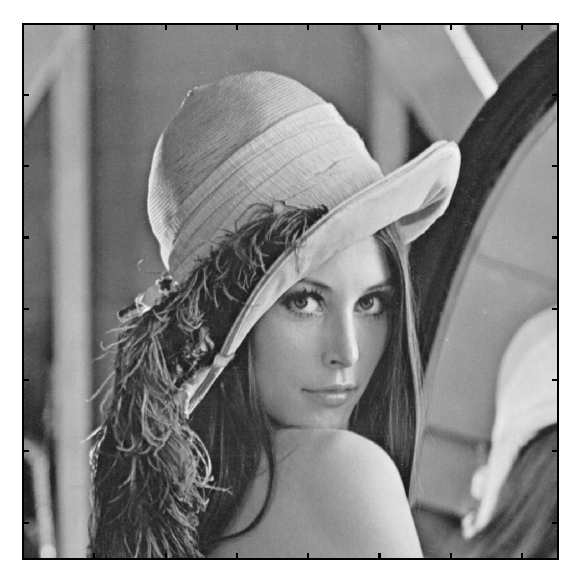
\includegraphics[width=.5\textwidth]{C:/Users/Massimo/Documents/Thesis/Thesis_PhD/lena_full.eps}
	\caption{\label{fig:lenafull} Image used as an object in the simulations.}
\end{figure}
\begin{figure}[H]
	\centering
	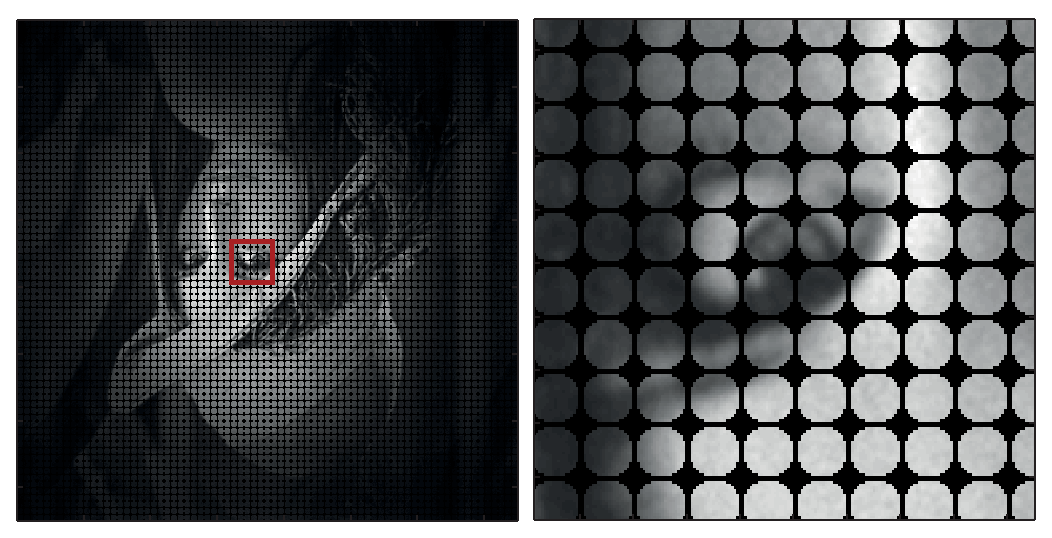
\includegraphics[width=.9\textwidth]{C:/Users/Massimo/Documents/Thesis/Thesis_PhD/rawlena.eps}
	\caption{\label{fig:rawlena10}Left: Example of a raw plenoptic 1.0 image. Right: Zoom on the raw image of the region indicated with the red square. Each lenslet is formed by 20 $\times$ 20 pixels. Each pixel represents a direction of the rays hitting the lenslet that produced the sub image.  }
\end{figure}
This raw image is the first parameterization of the light field and it is called the camera view. Pixels are arranged according to the positional coordinates, and each sub image contains the directional coordinates as shown in figures \ref{fig:rawlena10} and \ref{fig:arrayview}. \\
A second parameterization, known as the array view, is obtained by rearranging the pixels according to the directional coordinates \cite{ng2006digital}. The result is an array of N $\times$ N sub images, where N is the number of samples of the directional coordinates. Each sub image represents the point of view linked with a direction $(\theta_x, \theta_y)$. The array view can be seen in figure \ref{fig:arrayview1} and \ref{fig:arrayview1z} while the method to pass from the camera view to the array view is illustrated in figure \ref{fig:arrayview}. \\
\begin{figure}[H]
	\centering
	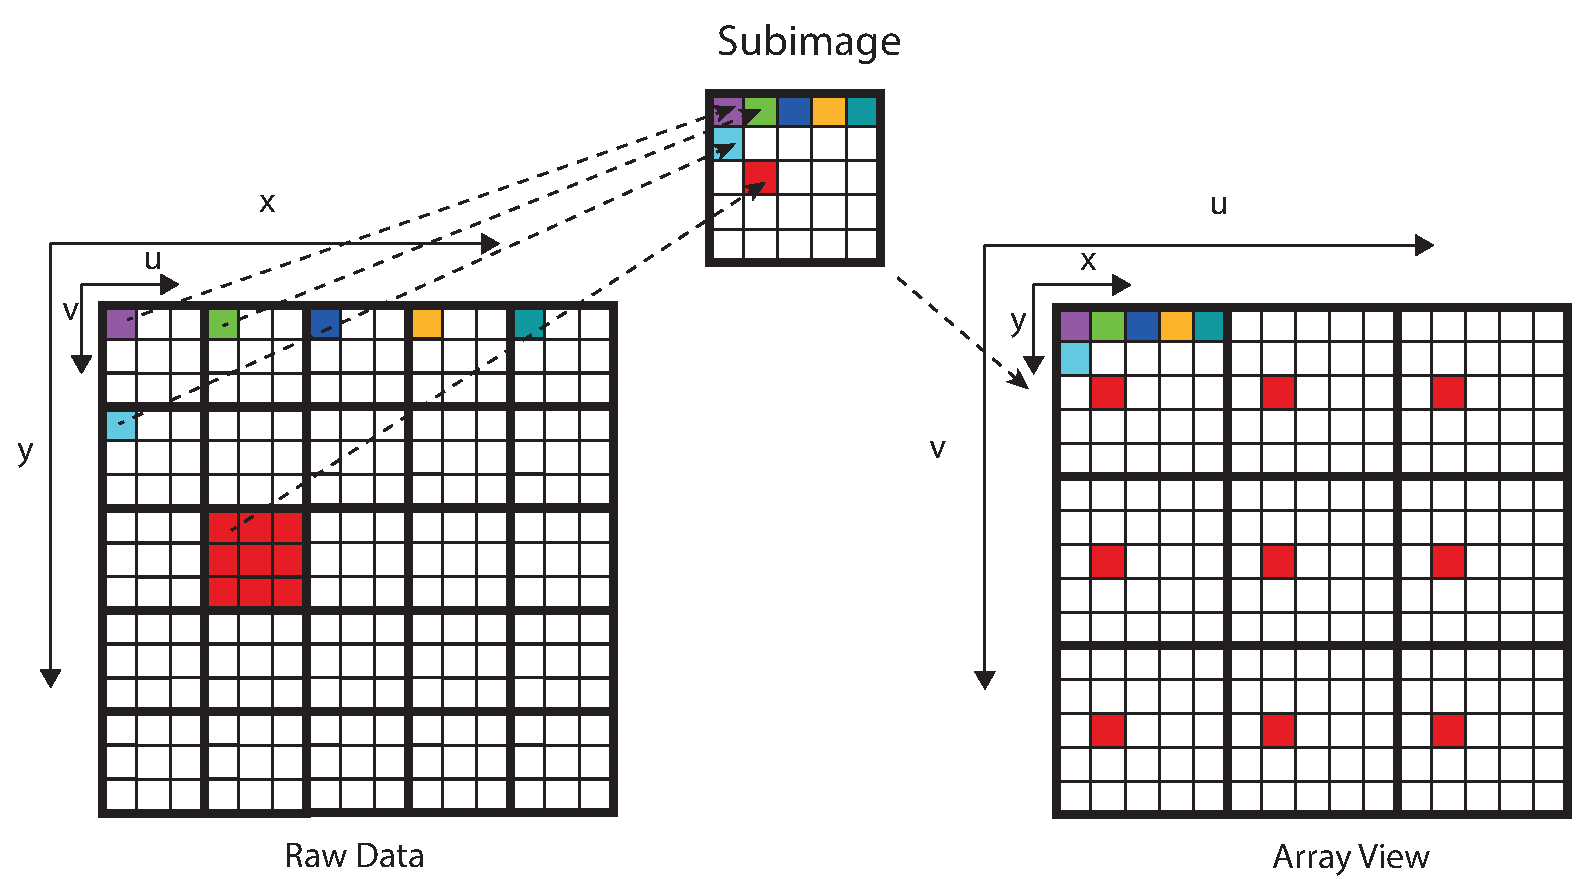
\includegraphics[width=.9\textwidth]{C:/Users/Massimo/Documents/Thesis/Thesis_PhD/imgformation.eps}
	\caption{\label{fig:arrayview}The array view is an array of the different point of view obtained rearranging the pixels according to the directional coordinates.  }
\end{figure}
An example of the array view parametrization of the raw image in figure \ref{fig:rawlena10} is shown in figure \ref{fig:arrayview1}.\\
The third and last parametrization of the light field is the 4-D radiance, a four dimensional function that represents radiance as a function of position and direction. \cite{levoy1996light}. This third parametrization is less intuitive but is very useful from a computational point of view since it is a four dimensional array, and every ray can be addressed by a set of four coordinates, or indices, as will be explained in detail in chapter \ref{chap:chapter4}.
\newpage
\begin{figure}[H]
	\centering
	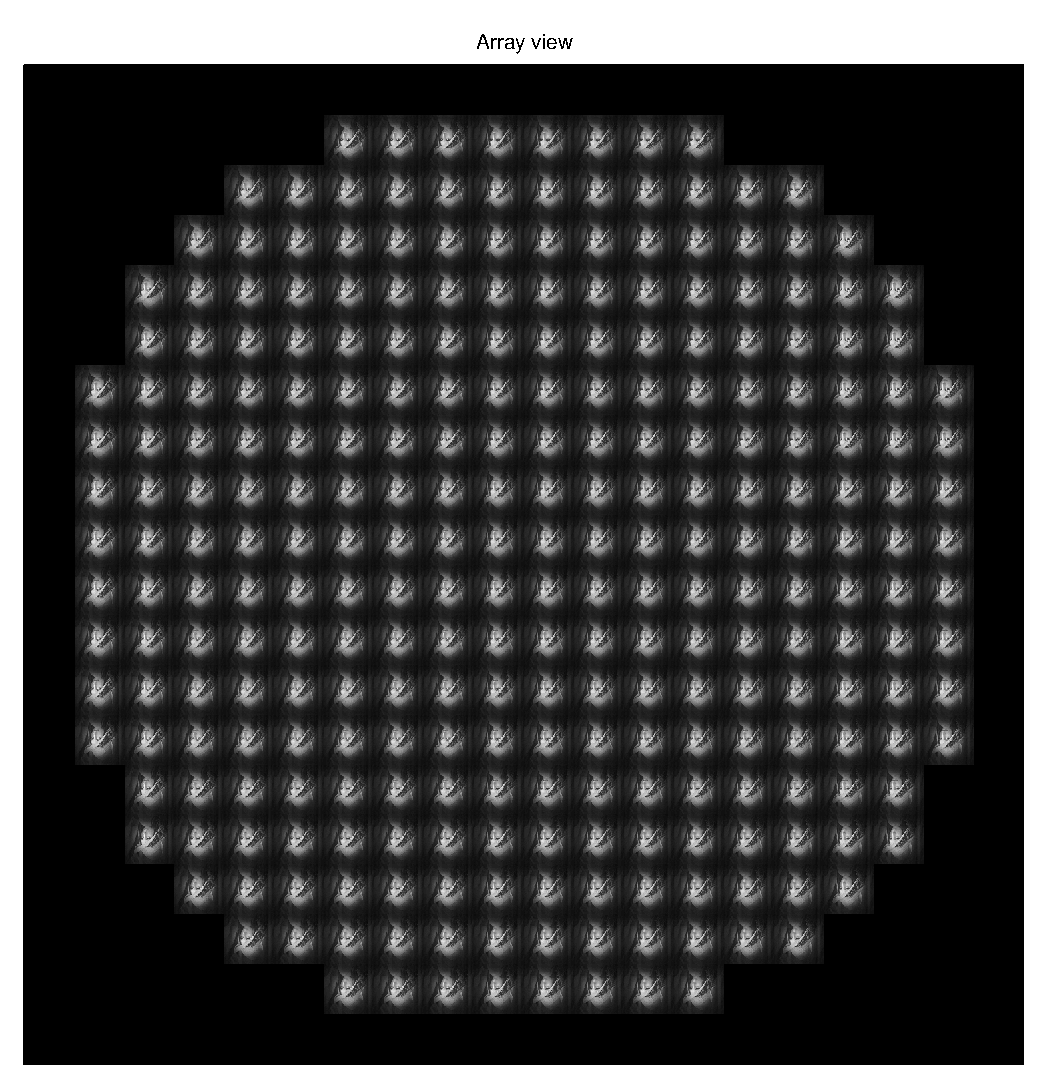
\includegraphics[width=.6\textwidth]{C:/Users/Massimo/Documents/Thesis/Thesis_PhD/arrayview.eps}
	\caption{\label{fig:arrayview1}Array view of the raw data shown in figure \ref{fig:rawlena10}.  }
\end{figure}
\begin{figure}[H]
	\centering
	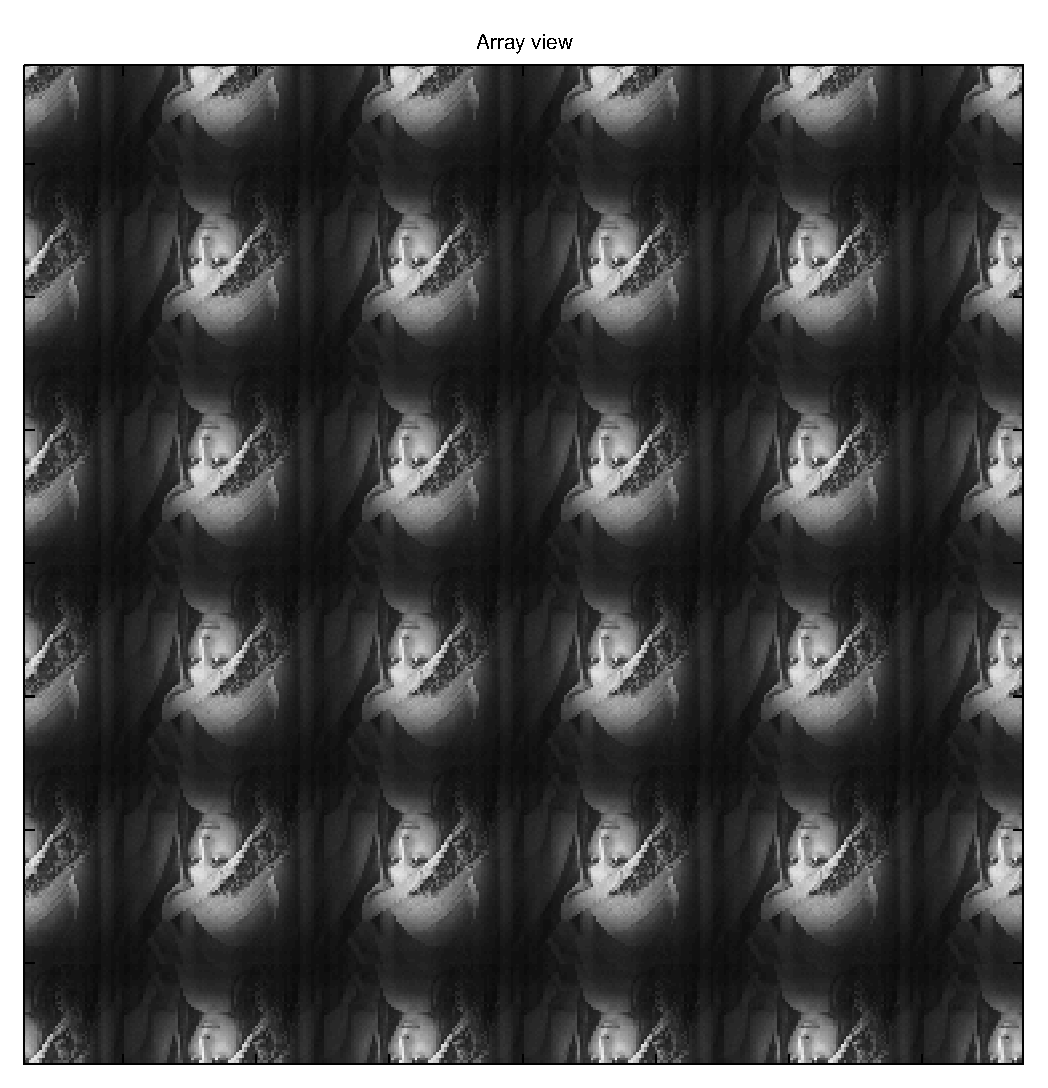
\includegraphics[width=.6\textwidth]{C:/Users/Massimo/Documents/Thesis/Thesis_PhD/arrayviewz.eps}
	\caption{\label{fig:arrayview1z}Zoom of the central part of the array view showing in detail the different points of views.  }
\end{figure}
\newpage
\section{Plenoptic 1.0 Rendering}
\label{sec:rendering1}
The act of de-codifying the information present on the sensor of the plenoptic camera in order to get an image is called rendering. 
In a conventional 2D image the intensity of each single pixel, corresponding to a position, is obtained by summing the contributions of all the rays of light converging to that point of the sensor \cite{georgiev2010focused} as shown in figure \ref{fig:render1}. This is equivalent to integrating over all possible directions for each position. 
\begin{figure}[H]
	\centering
	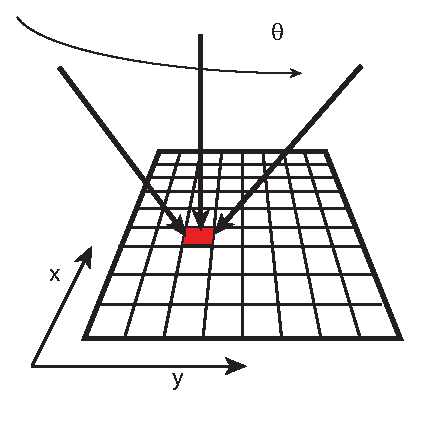
\includegraphics[width=.5\textwidth]{C:/Users/Massimo/Documents/Thesis/Thesis_PhD/rendering1.eps}
	\caption{\label{fig:render1} The intensity of a single pixel is obtained summing all the rays of light coming from all the possible directions.\cite{ng2006digital} }
\end{figure}
The same is valid for a computational image, where the integrations are made in post processing from the raw plenoptic data captured.
 If $L(x,y,u,v)$ is the sampled 4D light field, the radiance $E(x,y)$ on a pixel \textit{(x,y)} of the final rendered image will be given by integrating all the rays coming from all the sampled directions \textit{(u,v)} for any fixed point\textit{ (x,y)}. Following the work of Ng \cite{ng2006digital}:
\begin{equation}
\label{eq:rendering1}
I(x,y)=\dfrac{1}{z^2}\iint L(x,y,u,v)\mathscr{A}(u,v)cos^4\theta dudv
\end{equation} 
Where $z$ is the distance between the main lens and the sensor, $\theta$ is the angle formed by the rays and the sensor normal to the sensor surface and $\cos^4\theta$ is the vignetting factor. It takes into account the fact that the total light illuminating the sensor  declines moving outward  from  the  centre  of  the  image. The result is a relative darkening of the image toward 
its borders. This phenomenon can be well described by the so called "cosine fourth" law \cite{kerr2007derivation}. $\mathscr{A}(u,v)$ is an aperture function that limits the directions upon which integration takes place to the ones included in the aperture of the main lens. In the paraxial approximation, the $cos^4\theta$ term can be dropped as well as the $1/z^2$ term and equation \ref{eq:rendering1} becomes:
\begin{equation}
\label{eq:rendering2}
I(x,y)=\iint L(x,y,u,v)\mathscr{A}(u,v) dudv
\end{equation}
From a computational point of view, since the samples are discrete, the double integral becomes as a sum along the directional coordinates u and v. The total intensity of each pixel of the rendered image is then the sum of the intensities of the pixels that form the corresponding sub image divided by the number of pixels in the sub image. For a light field with N $\times$ N directional samples, the intensity $I(x,y)$ is given by:
\begin{equation}
\label{eq:rendering3}
I(x,y) = \dfrac{1}{N^2}\sum_{i=0}^N\sum_{j=0}^N L(x,y,i,j)
\end{equation}
This can be seen in the phase space where each pixel of the final image is made by the mean of all N directional samples \cite{georgiev2010focused}, as shown in figure \ref{fig:rendering2}.
 \begin{figure}[H]
 	\centering
 	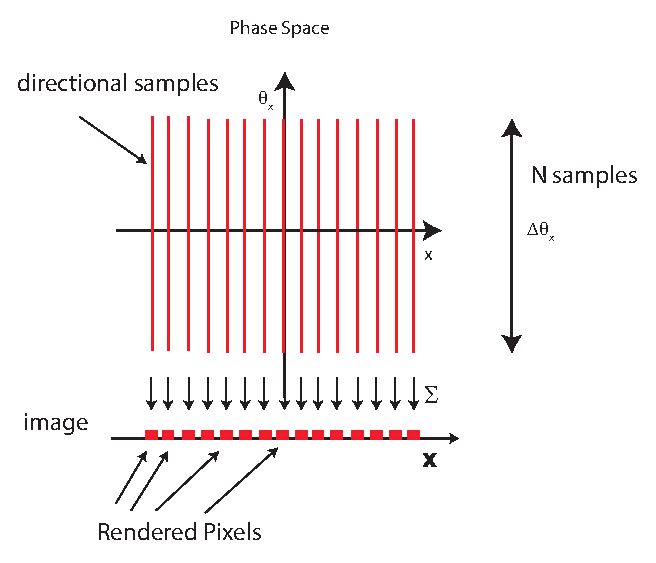
\includegraphics[width=.5\textwidth]{C:/Users/Massimo/Documents/Thesis/Thesis_PhD/renderingphase.eps}
 	\caption{\label{fig:rendering2} Rendering an image from plenoptic 1.0 raw data is equal to summing all the directional samples for each position. This process is shown for the $(x,\theta_x)$ slice of the phase space. \cite{georgiev2010focused} }
 \end{figure}
 From figure \ref{fig:rendering2} it can be noted that rendering an image from a light field captured by a plenoptic 1.0 camera causes a loss of resolution compared with the image collected by a conventional camera using the full sensor. Each pixel of the final image corresponds to one lenslet. Considering a plenoptic camera composed of a sensor with a resolution of 1000 $\times$ 1000 pixels and a micro lens array of 100 $\times$ 100 lenslets, each sub image will contain 10 $\times$ 10 directional samples. All these samples will contribute in computing the intensity of a single pixel, therefore there will be only one pixel per lenslet in the final image whose resolution is 100 $\times$ 100 pixels. This is the main limitation to plenoptic 1.0 cameras: the better the directional information is sampled, the more spatial resolution is lost \cite{georgiev2010focused, ng2006digital}. An example of a rendered image from a computer generated light field is shown in figure \ref{fig:renderlena}
 \begin{figure}[H]
 	\centering
 	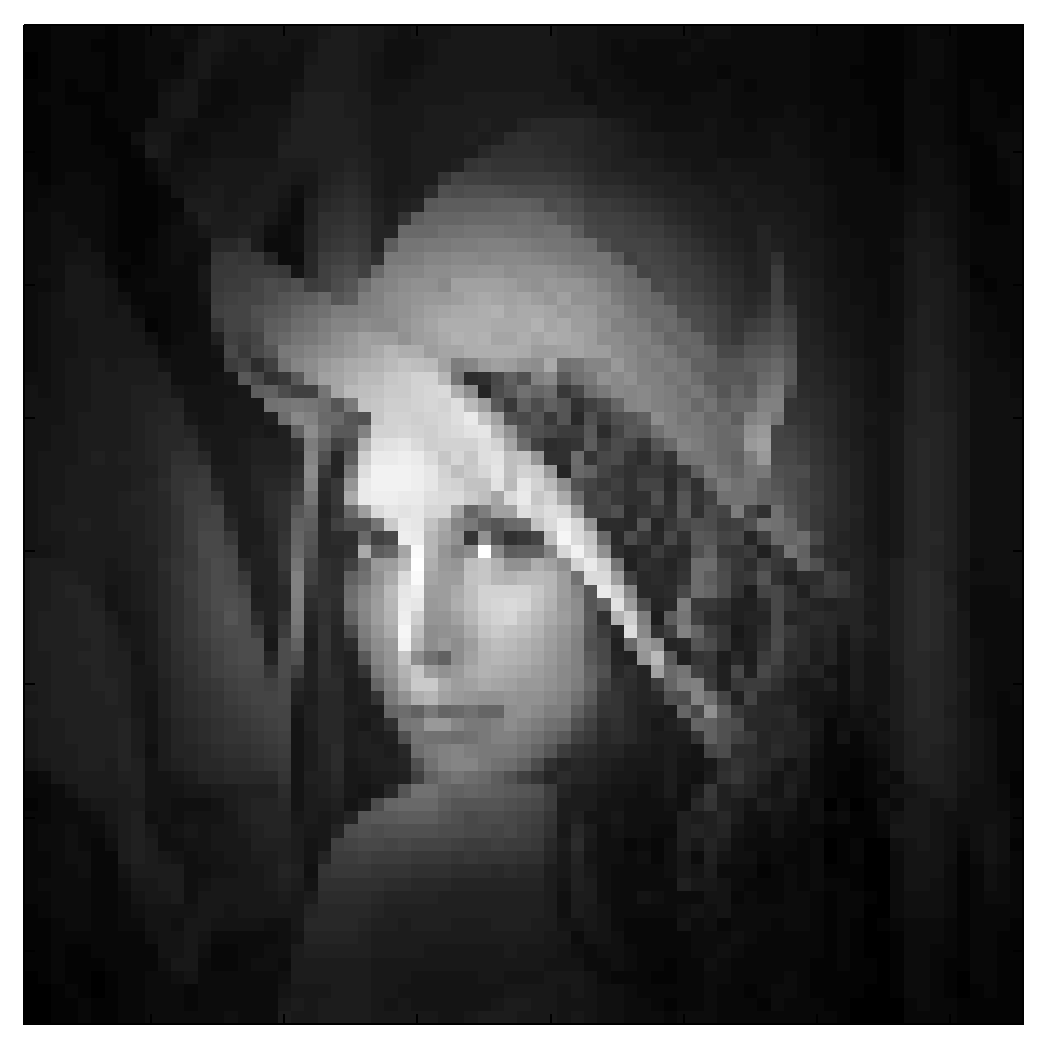
\includegraphics[width=.7\textwidth]{C:/Users/Massimo/Documents/Thesis/Thesis_PhD/renderlena.eps}
 	\caption{\label{fig:renderlena} rendered image from the raw data in figure \ref{fig:rawlena10}. Resolution is only 75 $\times$ 75 pixels.  }
 \end{figure}
 This loss of resolution arises from the fact that the lenslet array is not focused on the sensor and it produces on the sensor a blurred image \cite{georgiev2010focused}.
 \section{Plenoptic Camera 2.0}
 \label{sec:pleno20}
 A new kind of plenoptic camera, named focused plenoptic camera or plenoptic camera 2.0, has been proposed by Lumsdaine and Georgiev \textit{et al}. \cite{lumsdaine2008full,lumsdaine2009focused}. As shown in figure \ref{fig:plenoptic2} the plenoptic camera 2.0 is based on an array of micro lenses focused on the image plane of the main lens. In this configuration the sensor plane becomes conjugated with the main lens image plane. As will be discussed in the next sections, in a plenoptic 2.0 camera there is a flexible trade-off between angular and spatial resolution \cite{georgiev2010focused} leading to a full sensor resolution in the final image \cite{bishop2011full,georgiev2009resolution}. There are two possible configurations of the plenoptic 2.0 camera, as shown in figure \ref{fig:pleno201}. In both configurations each micro lens forms on the sensor a relay image of part of the main lens image. The position of the micro array is determined to satisfy the lens equation $1/a+1/b=1/f_{\mu}$, where $a$ is the distance from the main lens image plane to the micro array, $b$ is the distance from the micro array to the sensor plane and $f_{\mu}$ is the focal length of each micro lens. If $b$ is bigger than the focal length $f_{\mu}$ the camera is in a \textit{Copernican configuration} where the main lens image is a real image in front of the micro array, while if $b$ is smaller then $f_{\mu}$, the distance \textit{a} happens to be negative and the main lens image is formed behind the sensor plane. This is called \textit{Galilean configuration} and the micro array images a virtual main lens image (figure \ref{fig:pleno201}) \cite{georgiev2010focused}. 
 \begin{figure}[H]
 	\centering
 	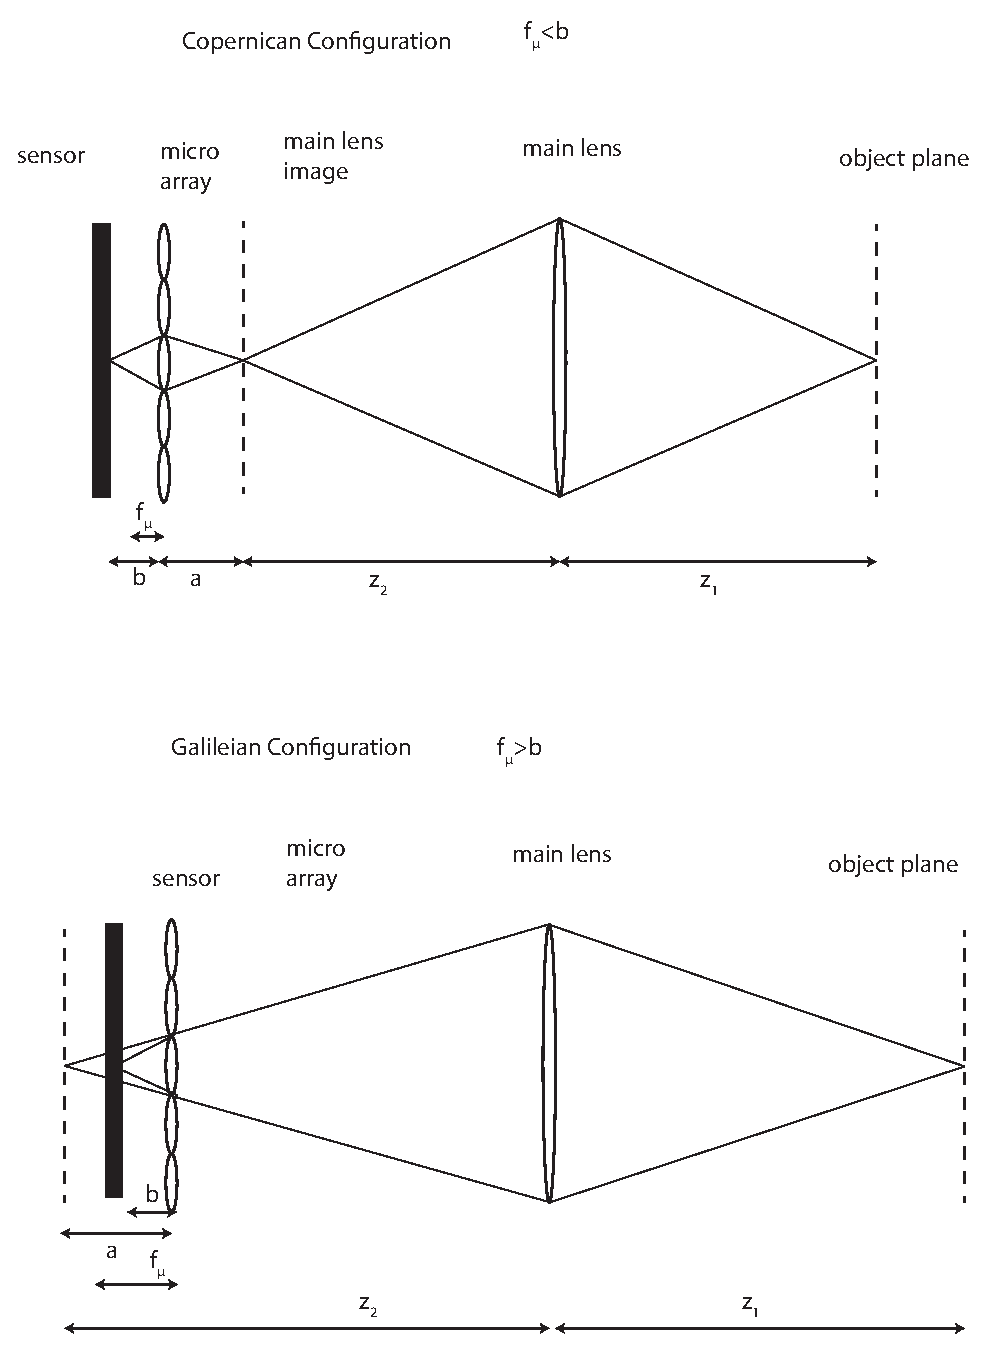
\includegraphics[width=.7\textwidth]{C:/Users/Massimo/Documents/Thesis/Thesis_PhD/plenoptic201.eps}
 	\caption{\label{fig:pleno201} If the main lens image is formed in front of the micro array the configuration is called \textit{Copernican}, top, and the focal length of the micro array is smaller then the distance b. If the main lens image is formed behind the micro array the configuration is \textit{Galilean}, on the bottom, and the focal length of the micro array is bigger then the distance b. }
 \end{figure}
 For both configurations the magnification of the micro array stage is:
 \begin{equation}
 \label{eq:pleno20}
 m=\dfrac{b}{a}
 \end{equation}
 The ratio between the distances $a$ and $b$ plays a crucial role in sampling the light field in the plenoptic camera 2.0. Figure \ref{fig:rawpleno20} shows a raw plenoptic 2.0 image of a point source acquired through simulation (as discussed in chapter \ref{chap:fresnel}). The system is composed of a main lens with a focal length of 60 mm, in a 2f configuration and a micro array made of $150 \mu m$ diameter lenslets with focal length of 5.3 mm. The distances \textit{a} and \textit{b} are set in order to have a magnification \textit{m} of 0.3. In this configuration each point of the main lens image is sampled by three lenslets and each sub image corresponds to a point of view of the object. The number of points of view depends on the magnification of the micro array stage. Hence, in order to have more than one point of view recorded it is necessary that the magnification \textit{m} is less than one. Looking at figure \ref{fig:rawpleno20} the raw image is composed of a 3 $\times$ 3 matrix of sub images, three points of view in the x direction and three along the y direction. Figure \ref{fig:rawpleno203} shows central 5 $\times$ 5 sub images in the raw data. The central sub image records the direction corresponding to the central point of view, indicated in both figures with the number 2. The lenslets on the left and on the right of the central one record the directions corresponding to the point of views from the left, indicated with 1 in figure \ref{fig:rawpleno202}, and right, indicated with 3. The sub images 1 and 3 are shifted towards the outer edge of the sub image. This happens as an effect of the change in the point of view as well as because the sub images are flipped upside down as a consequence of the imaging law.
  \begin{figure}[H]
 	\centering
 	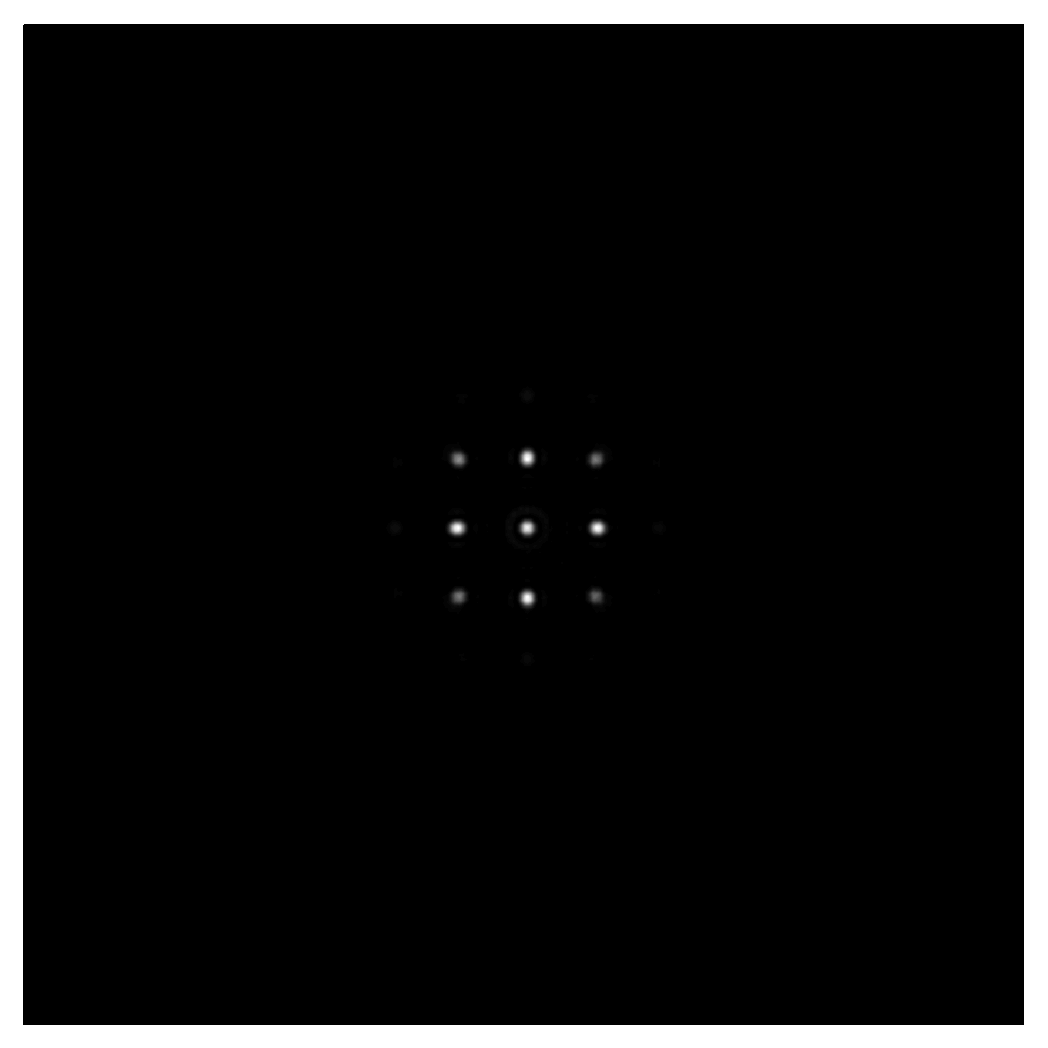
\includegraphics[width=.5\textwidth]{C:/Users/Massimo/Documents/Thesis/Thesis_PhD/rawimage.eps}
 	\caption{\label{fig:rawpleno20} Raw data of a point source sampled by a plenoptic 2.0 system with a magnification of the micro array stage equal to 0.3. Data acquired with numerical simulations. }
 \end{figure}
 \begin{figure}[H]
 	\centering
 	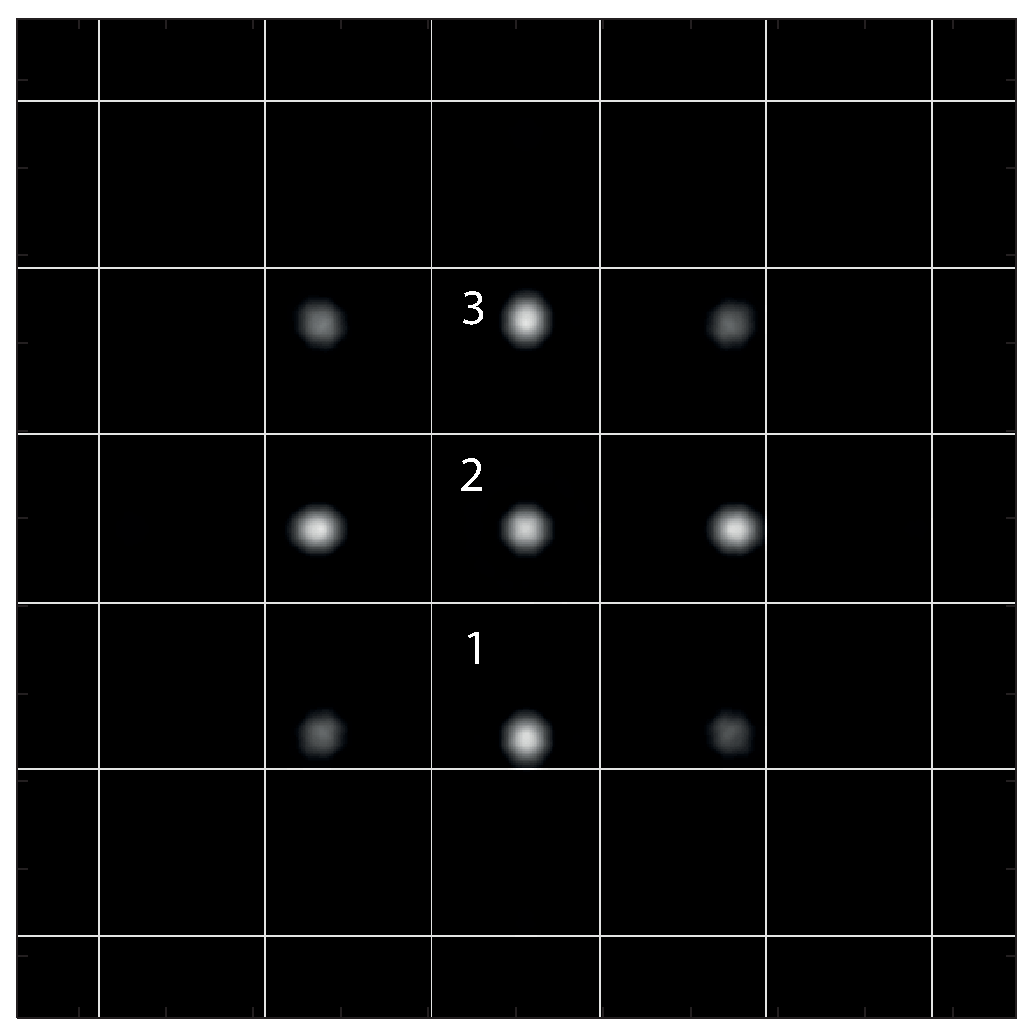
\includegraphics[width=.5\textwidth]{C:/Users/Massimo/Documents/Thesis/Thesis_PhD/rawzoom.eps}
 	\caption{\label{fig:rawpleno203} Zoomed raw data of a point source sampled by a plenoptic 2.0 system with a magnification of the micro array stage equal to 0.3. Data acquired with numerical simulations. The grid represent the boundaries of each sub image to show how the point of view of the point source changes across the lenslets. The sub images are shifted by a quantity proportional to the position of the lenslet in the array.  }
 \end{figure}
  \begin{figure}[H]
  	\centering
  	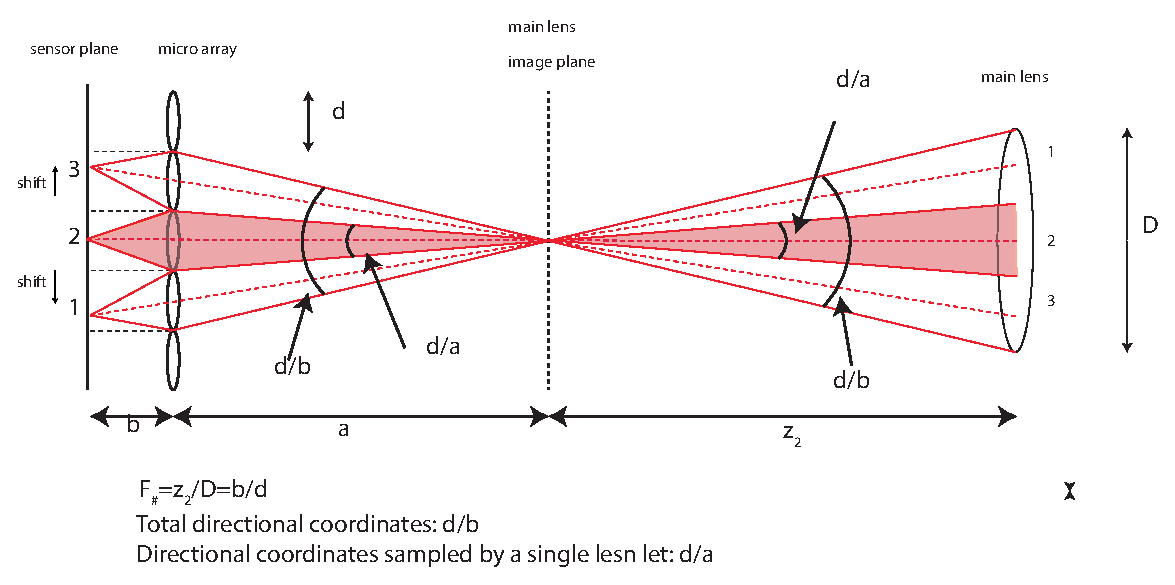
\includegraphics[width=1  	\textwidth]{C:/Users/Massimo/Documents/Thesis/Thesis_PhD/LFsampling.eps}
  	\caption{\label{fig:rawpleno202}Sampling of the light field by a plenoptic 2.0 system with a magnification of \textit{m=0.3}. For simplicity the one dimensional case is shown. Each micro lens has a diameter equal to d, a focal length $f_{\mu}$, and images the main lens image on the sensor according to the lens law $1/a+1/b=1/f_{\mu}$ The total range of directions that can be sampled is given by $d/b$. Each lenslet samples a sub set of directions equal to $d/a$ as a single direction. The range of directions shown in red are sampled by the central micro lens as a single point of view. The angular resolution is therefore \textit{d/a} and the total number of directional samples is \textit{a/b = 1/m}. In the specific case shown is 3. }
  \end{figure}
  As in the 1.0 case, the f-number of the micro lenses matches the f-number of the main lens.
 With reference to figure \ref{fig:rawpleno202} because of the f-number matching condition the total number of directions captured by the main lens is defined as $\Theta=D/z_2=d/b$ where D is the aperture of the main lens, $z_2$ the distance of the main lens image, d is the diameter of the lenslet and b is the distance between the lenslet and the sensor. The amount of directions captured by a single lenslet is equal to $p=d/a$. Hence the range sampled by the single lenslet with respect to the total range of directions in the light field is:
 \begin{equation}
 \label{eq:magnification}
 \dfrac{p}{\Theta}=\dfrac{d}{a}\dfrac{b}{d}=m
 \end{equation} 
 Hence:
  \begin{equation}
  \label{eq:magnification2}
  p=\dfrac{b}{a}\Theta=m\Theta
  \end{equation}
  Therefore the magnification of the lenslet array determines the angular resolution of the plenoptic 2.0 system. In the case illustrated in figures \ref{fig:rawpleno201} and \ref{fig:rawpleno202} for each position x on the main lens image plane, 3 directions are sampled. Since the main lens image is scaled by the lenslets by a factor of $m$, the resolution of the rendered image will be $b/a$ times the resolution of the full sensor. This fact implies that the spatio-angular trade off of the plenoptic 2.0 camera is not fixed by the number of micro lenses, but it is determined by the optical geometry of the micro lens stage, and is fully determined by the magnification $m=b/a$. The more samples of the directional coordinates, the less will be the spatial resolution of the rendered image. In section \ref{sec:phase2.0} a more rigorous proof of this will be given.
  Figure \ref{fig:rawpleno201} shows the effect of magnification on the raw image of a point source. If the magnification is 1, the main lens image is replicated on the sensor under only one lenslet. No further information is given by the micro array stage. The whole range of directions is sampled by a single lenslet and with only one point of view it is not possible to recover the directional information. In order to have more than one point of view, \textit{m} should be at least 0.5. In this case the point source is replicated under a total of four lenslets giving 2 $\times$ 2 points of view to render the image. If the magnification decreases further, the number of points of view increases. The directional information in plenoptic 2.0 is recorded not by a single lenslet like in the 1.0 case, but across many lenslets, since each point of the object plane is imaged by a number of lenslets proportional to the inverse of the magnification \ref{eq:pleno20}. Each lenslet samples a part of the directional coordinates contained into the solid angle \textit{d/a}. The more point of view that are present, the smaller will be the solid angle \textit{d/a}, and therefore, the better will be the angular resolution. \cite{lumsdaine2009focused}
   \begin{figure}[H]
  	\centering
  	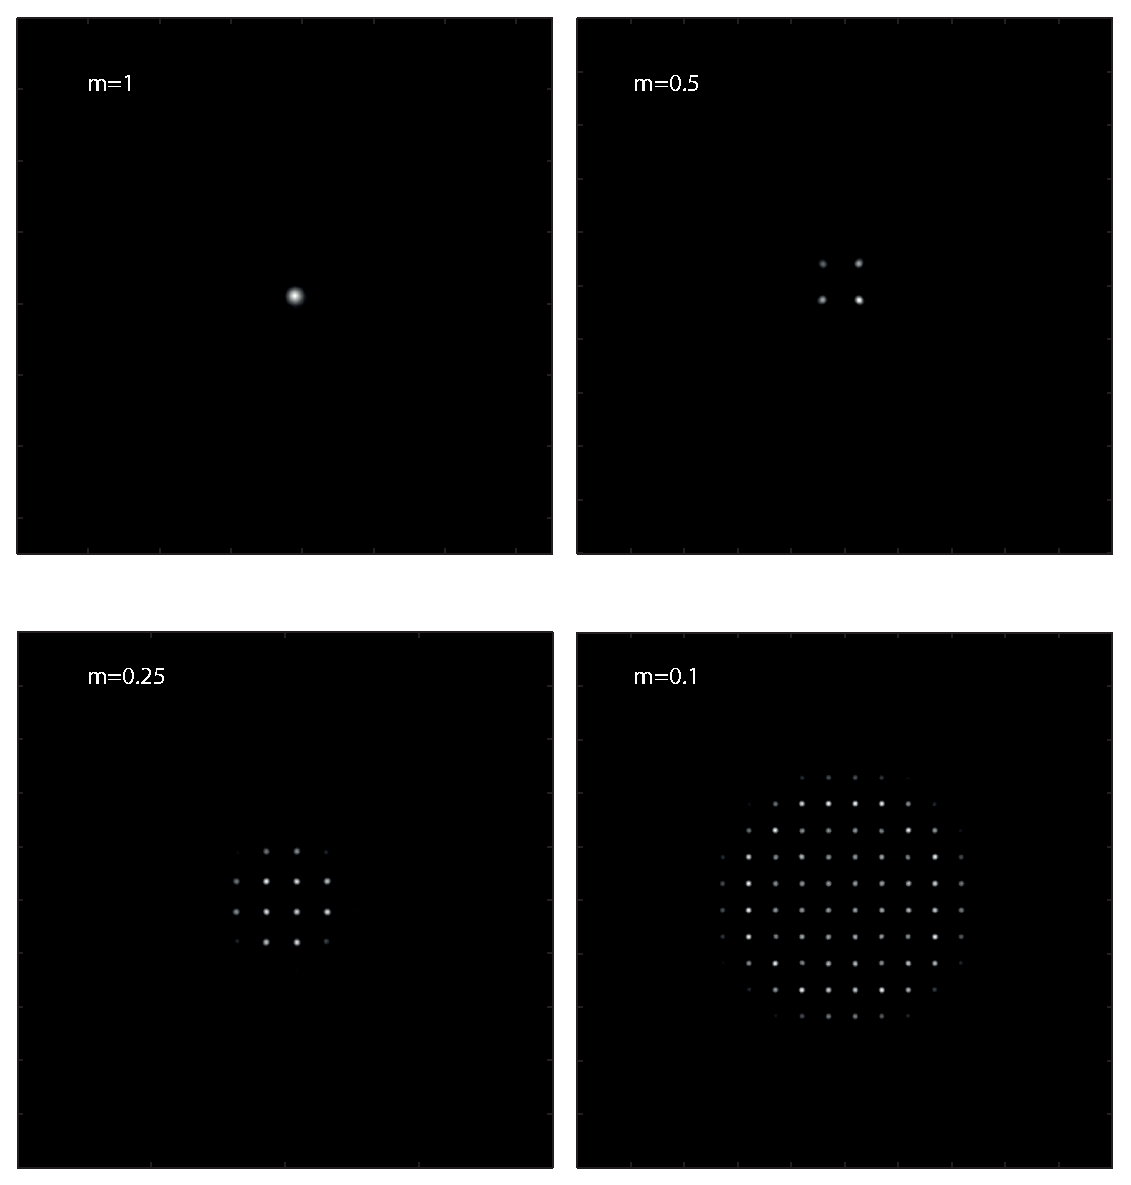
\includegraphics[width=.8\textwidth]{C:/Users/Massimo/Documents/Thesis/Thesis_PhD/rawimages.eps}
  	\caption{\label{fig:rawpleno201}Raw images of a point source simulated with different magnifications. From top left to bottom right: \textit{m = 1, m = 0.5, m= 0.25, m = 0.1}. }
  \end{figure}
  \newpage
  \section{Plenoptic Camera 2.0: a Geometrical Optics Analysis}
  \label{sec:phase2.0}
  This section provides a mathematical proof of the concepts introduced in section \ref{sec:pleno20}. The mathematical model of Light Field sampling in plenoptic 2.0 has been developed by Lumsdaine and Georgiev \cite{lumsdaine2009focused,lumsdaine2008full}. The goal of this chapter is to express the intensity profile present on the sensor as a function of the light field at the focal plane of the main lens. The intensity on the sensor is given by integrating for each pixel along all the rays, or the directions, the radiance captured by the sensor in analogy with what was discussed in \ref{sec:rendering1}:
  \begin{equation}
 	\label{eq:phase201}
 	I(x,y)=\iint_{\theta_x, \theta_y}L(x,y,\theta_x,\theta_y) d\theta_xd\theta_y
  \end{equation} 
  For simplicity only one positional coordinate \textit{x} is considered, and its corresponding direction will be described by a new coordinate called \textit{momentum}, in analogy with Hamiltonian mechanics, defined as:
  \begin{equation}
	\label{eq:momentum2}
	p_x = n\theta_x
  \end{equation}
  where \textit{n} is the refractive index of the medium of propagation, assumed to be homogeneous. The reason of this change in coordinates is that using the momentum \textit{p} the transformations matrix of the optical elements are invertible and the calculations are simpler \cite{guillemin1990symplectic}. The one dimensional intensity profile is then equal to:
  \begin{equation}
  \label{eq:1Dintensity}
  I(x)=\int_{p_x}L(x,p_x) dp_x
  \end{equation} 
  In the phase space the rays composing the light field, will be represented by points with coordinates $(x,p_x)$. Given a ray $\overrightarrow{X_0}=(x,p_x)$, it is possible to define a ray transfer matrix \textit{A} describing the transformation the ray undergoes while propagating in an optical system as:
  \begin{equation}
  \label{eq:transmatrix1}
  \overrightarrow{X_1}=A\overrightarrow{X_0}
  \end{equation}
  Where $\overrightarrow{X_1}$ is a vector representing the ray after the transformation \textit{A}. The transformation matrix has the property of having its determinant equal to unity, \textit{det(A)=1}, and is invertible. It is therefore possible to express the ray $\overrightarrow{X_0}$ as a function of $\overrightarrow{X_1}$ as:
   \begin{equation}
   \label{eq:transmatrix2}
   \overrightarrow{X_0}=A^{-1}\overrightarrow{X_1}
   \end{equation}
   The same considerations can be made for the full set of rays composing the light field. In the assumption of zero loss during the propagation, the total light field \textit{L} is conserved, and $L(\overrightarrow{X_0})$ equals $L(\overrightarrow{X_1})$. Therefore:
   \begin{equation}
   \label{eq:transmatrix3}
   L_1(\overrightarrow{X_1})=L_0(\overrightarrow{X_0})
   \end{equation} 
   Because of equation \ref{eq:transmatrix1} the Light Field at the position $\overrightarrow{x_1}$ is :
   \begin{equation}
   \label{eq:transmatrix4}
   L_1(A\overrightarrow{X_0})=L_0(\overrightarrow{X_0})
   \end{equation}
   For the ray $\overrightarrow{X_1}=A\overrightarrow{X_0}$:
   \begin{equation}
   \label{eq:transmatrix8}
   L_1(\overrightarrow{X_1})=L_0(A^{-1}\overrightarrow{X_1})
   \end{equation}
   For the generic ray $\overrightarrow{X}$ the light field transformation formula becomes:
   \begin{equation}
   \label{eq:transmatrix5}
   L_1(\overrightarrow{X})=L_0(A^{-1}\overrightarrow{X})
   \end{equation}
   Equation \ref{eq:transmatrix5} shows the link between the light field at a plane, with the same light field after an arbitrary optical transformation.
     With reference to figure \ref{fig:basystem} a single lenslet of diameter \textit{d} is shown and the light field at the sensor plane $L_b(x,p_x)$ is expressed as a function of the coordinates of the light field at the main lens image plane $L_a(x,p_x)$. The link between the two light fields is given by equation \ref{eq:transmatrix5}. According to geometrical optics, and as is explained in Georgiev \textit{et al.}\cite{georgiev2011plenoptic}, the optical transfer matrix $A_{ab}$ from the main lens image plane and the sensor is the composition of two free space propagation matrices and a lens matrix.
      \begin{figure}[H]
      	\centering
      	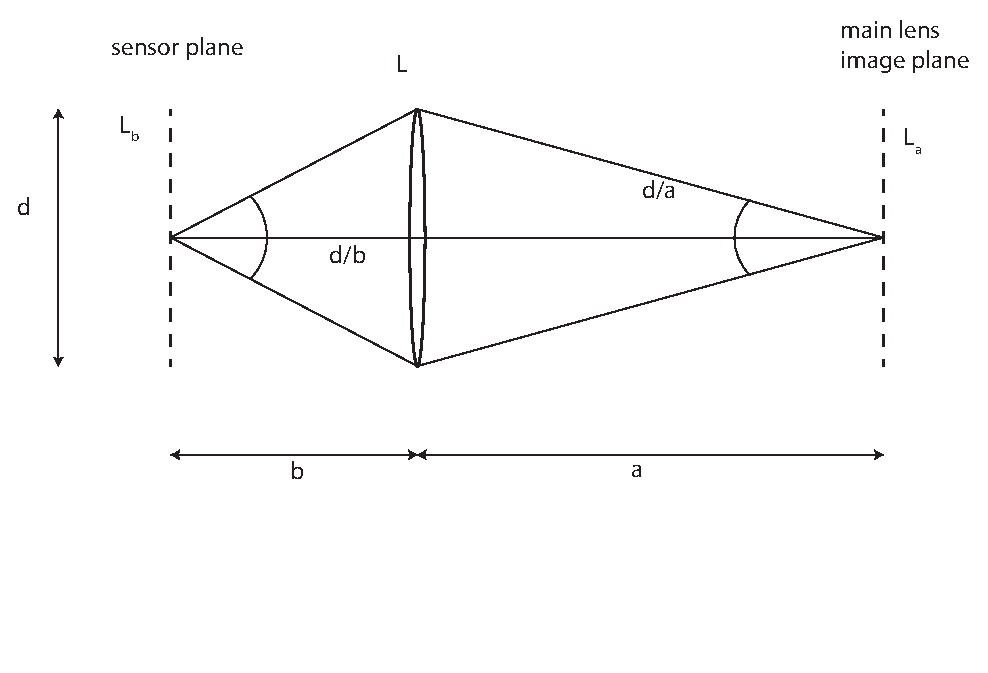
\includegraphics[width=.7\textwidth]{C:/Users/Massimo/Documents/Thesis/Thesis_PhD/singlelens.eps}
      	\caption{\label{fig:basystem} System formed by a single lenslet. The rays at the main lens image plane are transformed into the rays at the sensor plane by the lenslet. The transformation can be described by a matrix \textit{A}. }
      \end{figure}
Therefore:
   \begin{equation}
   \label{eq:transmatrix6}
   A_{ab}=
   \begin{bmatrix}
   1 & b \\ \\
   0 & 1
   \end{bmatrix}
   \begin{bmatrix}
  1 & 0 \\ \\
  -\dfrac{1}{f_{\mu}} & 1
   \end{bmatrix}
   \begin{bmatrix}
   
   1 & a \\ \\
   0 & 1
   \end{bmatrix}
   =
   \begin{bmatrix}
   -\dfrac{b}{a} & 0\\\\
   -\dfrac{1}{f_{\mu}}&-\dfrac{a}{b}
     \end{bmatrix}
   \end{equation}
   Its inverse is:
   \begin{equation}
   \label{eq:transmatrix7}
   A_{ab}^{-1}=
   \begin{bmatrix}
   -\dfrac{a}{b} & 0\\\\
   \dfrac{1}{f_{\mu}}&-\dfrac{b}{a}
   \end{bmatrix}
   \end{equation}
     Applying the inverse $A^{-1}$ matrix to equation \ref{eq:transmatrix5} and substituting into the integral in equation \ref{eq:phase201}, the intensity on the sensor behind a single lenslet is: 
   \begin{equation}
   \label{eq:radiance}
   	I(x)=\int_{p_x}L_a(-\dfrac{a}{b}x,-\dfrac{b}{a}p_x -\dfrac{1}{f}x) dp_x
   \end{equation}
   From figure \ref{fig:basystem}, for a single spatial coordinate x on the main lens image plane the integration takes place on a range of directional coordinates $p_x$ equal to $d/b$ and the result is:
   \begin{equation}
   \label{eq:radiance2}
   I(x)=\dfrac{d}{b}L_a(-\dfrac{a}{b}x, -\dfrac{1}{b}x) 
   \end{equation}
   From equation \ref{eq:radiance2} the micro lens maps the spatial coordinates on the main lens image plane to the sensor with a scaling factor equal to the magnification $m=b/a$. Therefore the resolution of the sampled light field on the sensor is $b/a$ times the resolution of the sensor. The directional coordinates are mapped as $x/b$. If the lenslet diameter is $d$ then the maximum number of directional coordinates sampled by one lenslet is equal to the f-number of the lenslet $d/b$. Figure \ref{fig:basystem} shows how a single micro lens samples the radiance from a single point X on the main lens image plane. Each pixel of the micro lens image samples a single position X and a span of $d/a$ directional coordinates $p_x$. The same position X is sampled also by other micro-lenses as shown in figure \ref{fig:phaseba}, but since each micro lens only captures $d/a$ samples of the directional coordinates, each lenslet samples a different portion of the total span of directional coordinates contained in the light field.
   \begin{figure}[H]
   	\centering
   	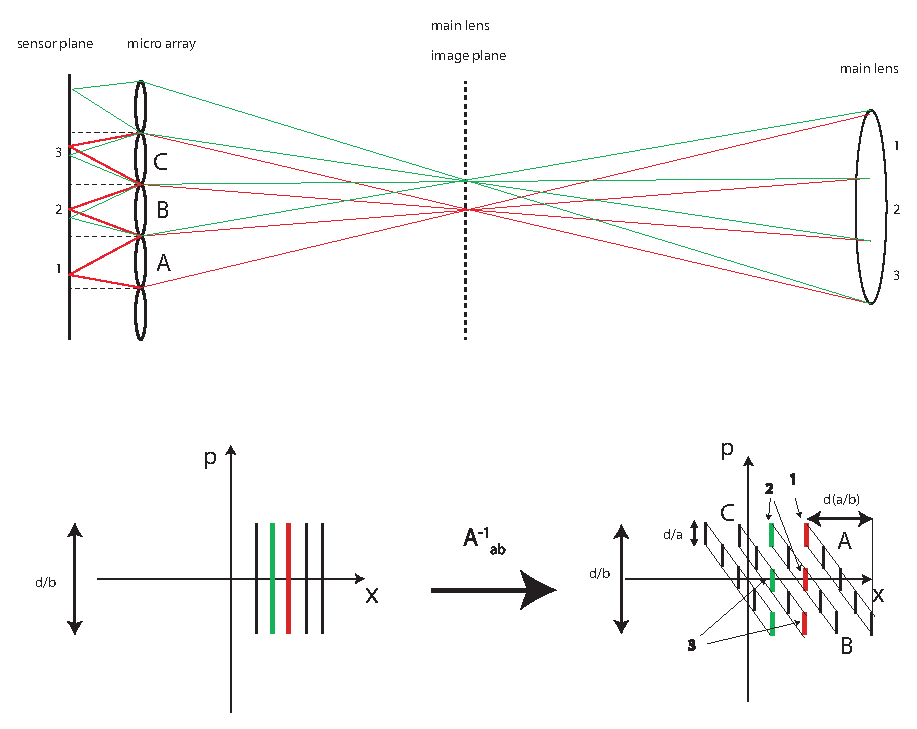
\includegraphics[width=1\textwidth]{C:/Users/Massimo/Documents/Thesis/Thesis_PhD/smapling1.eps}
   	\caption{\label{fig:phaseba} Sampling of the light field by plenoptic 2.0 camera. For each of the two points represented, red and green, The total range of directional coordinates are sampled by three  different lenslets. For one position three directions are sampled, with a resolution of d/a. Therefore the directional sampling in plenoptic 2.0 is made across many lenslets. This can be seen in the phase space. Lenset B and C sample 2 directions indicated with the same number in the ray diagram and the phase space. Lens let A only samples one direction of the red point.   }
   \end{figure}
   \section{Plenoptic 2.0 Rendering}
   \label{sec:rendering201}
   The basic rendering in plenoptic 2.0 cameras is still made by integrating all directions associated to a single position, as shown \ref{eq:pleno20}. The difference with plenoptic 1.0 rendering is that this time the directional coordinates for a single position, $d/b$, are recorded across many lenslets, each sampling $d/a$ coordinates and as a consequence of that, the integration takes place across all of these micro lenses \cite{georgiev2006light}. The basic rendering process is shown in figure \ref{fig:render20}.
   \begin{figure}[H]
   	\centering
   	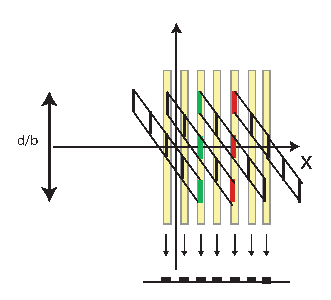
\includegraphics[width=.5\textwidth]{C:/Users/Massimo/Documents/Thesis/Thesis_PhD/rendering20b.eps}
   	\caption{\label{fig:render20} Image rendering with the focused plenoptic camera. One pixel of the rendered image is given by the integration on all the directions $d/b$ associated with a given position. The integration takes place across the lenslet and is represented by the vertical lines. Each lenslet is represented by the diagonal lines. }
   \end{figure}
   Rendering an image in plenoptic 2.0 is more complicated and less intuitive then the 1.0 case, therefore a more detailed analysis of plenoptic 2.0 rendering will be given in chapter \ref{chap:chapter5}.
   \section{Conclusions}
   In this chapter a general view of plenoptic imaging systems behaviour and characteristics was given. It is based on results already presented in the literature and it has the scope to put order in a new field where the literature is often fragmented and incomplete. It was introduced the concept of plenoptic function, as a function to describe the full set of information contained in the light. The concept light field was also presented as a four dimensional parametrization of the plenoptic function. Each ray of light is completely identified by a set of four coordinates, two spatial and two directional coordinates. This representation of the bundle of rays reaching the camera is very useful under a computational point of view since each ray of light can be represented as a point in the phase space. In the phase space an optical transformation is described by a optical transfer matrix with the property of having the determinant equal to one and to be invertible. In this way it is possible to give a mathematical description of the behaviour of the plenoptic camera and to put the basis for the ray tracing algorithms that will be presented in the following chapters.
   Two different types of plenoptic camera were described, the plenoptic 1.0 and 2.0. A detailed description of the how these two classes of devices record the light filed was given, pointing out the main differences in the performances of the two configurations.
   The main original contribution to the field given by this chapter is that for the first time a complete review of the characteristic of plenoptic camera 1.0 and 2.0 was given. This chapter represents a link between many pieces of work on plenoptic imaging and covers all the aspects of this new field providing a good overview of all the general aspects of plenoptic imaging.
   \nomenclature{$L$}{Light Field}
   \nomenclature{$x$}{Spatial coordinate}
   \nomenclature{$y$}{Spatial coordinate}
   \nomenclature{$z$}{Distance on the optical axis}
   \nomenclature{$v$}{Directional coordinate}
   \nomenclature{$u$}{Directional coordinate}
   \nomenclature{$a$}{Distance from the main lens image to the micro array}
   \nomenclature{$b$}{Distance from the micro array to the sensor}
   \nomenclature{$f$}{Focal length of the main lens}
   \nomenclature{$f_{\mu}$}{Focal length of the micro lens}
   \nomenclature{$d$}{Aperture diameter}
   \nomenclature{$\overrightarrow{X}$}{Vector representing the ray of light}
   \nomenclature{$A$}{Transformation matrix}
   \nomenclature{$A^{-1}$}{Transformation matrix}
   \nomenclature{$m$}{Magnification}
   \nomenclature{$D$}{Aperture diameter of the main lens}
   \nomenclature{$I$}{Intensity of the optical field}
   \nomenclature{$E$}{Radiance}
\chapter{Fresnel Simulation Toolbox}
\markboth{\MakeUppercase{Fresnel Simulation Toolbox}}{}
\label{chap:fresnel}
\section{Introduction}
\label{sec:intro}
This chapter describes a MATLAB simulation toolbox developed as a part of this doctorate project in order to investigate the potential of plenoptic imaging for biomedical and microscopy applications with particular interest in its behaviour at the diffraction limit. In literature are present many works on simulating plenoptic imaging devices. Plenoptic systems have been studied through simulation extensively. Until recently these studies have focussed on a geometrical optics approach, however in this project the focus is on investigating plenoptic systems biomedical and microscopy applications for which the performance at high resolution needs to be studied; hence diffraction cannot be ignored. Over the duration of this project there have been other research groups that have studied plenoptic systems under wave optics, including a wave optics analysis of plenoptic 1.0 systems, such as Schroff \textit{et al.} \cite{shroff2012high,shroff2013image} and Trujillo-Servilla \textit{et al.} \cite{birch2012depth} and a Fourier optics approach of the diffraction limit of a digital camera, Farrell \textit{et al.} \cite{farrell2012digital}. The growing interest in this aspect of plenoptic systems over the past few years is a product of the increasing interest in plenoptic systems overall and its new potential applications. In this work a Fresnel optics approach has been applied to a plenoptic camera with the purpose of understanding how the light field is recorded and to define some guidelines to design a working setup. Particular attention has been given to the behaviour of the system at its diffraction limit, a subject that has never been explicitly treated in literature. In this chapter four different methods to simulate light propagation in an optical system will be discussed and their performance compared in term of accuracy of the results, noise and computational effort.
A Fresnel optics approach has been chosen because the simulation tool to describe a plenoptic imaging system needs to have the following requirements:
\begin{itemize}
	\item it has to preserve the phase of the optical field propagating in order to preserve directional information of the rays of light;
	\item it has to take into account the effects of diffraction;
	\item it has to be adaptable in order to easily change the characteristic of the optical system, trying various configurations, keeping the operator based approach of ray tracing.
\end{itemize}
To address these features, a wave optics simulation toolbox has been designed and developed. Most of the existing literature on simulating plenoptic system are based on ray tracing techniques \cite{thurow2013recent,lynch2011development,lynch2012three,ng2006digital,levoy1996light}. The advantages of using ray tracing is that the transformations that rays undergo during the propagation can be described by two basic linear operators and compositions of them. These are the free space propagation and the lens operator. In developing the wave optics simulation this principle has been kept, and two operators have been defined: propagation and lens. Four different types of propagation operators have been described and compared. In analogy with ray tracing an optical system has been simulated using compositions of the two simple operators. In developing this platform all the media composing the system have been considered as linear, isotropic, homogeneous and non dispersive. 
\section{Scalar Theory of Diffraction}
\label{sec:scalar}
The term diffraction has been defined by Sommerfeld as any deviation of light rays from rectilinear paths which cannot be interpreted as reflection or refraction. \cite{sommerfeld1954optics}.The complex vectorial equations describing wave propagation in three dimensional space can be simplified into a set of scalar equations using the Scalar Theory of Diffraction as explained by Goodman \cite{goodman2005introduction}.
The starting point is given by Maxwell's Equations in absence of sources of electrical field of magnetic dipoles:\\
\begin{equation}
\label{eq:maxwell}
\begin{matrix}
	\nabla\times\overrightarrow{E}=-\mu\dfrac{\partial\overrightarrow{H}}{\partial t}\\
	\\
	\nabla\times\overrightarrow{H}=\epsilon\dfrac{\partial\overrightarrow{E}}{\partial t}\\
	\\
	\nabla\cdot\epsilon\overrightarrow{E}=0\\
	\\
	\nabla\cdot\mu\overrightarrow{H}=0\\
	\end{matrix}
\end{equation}
where $\overrightarrow{E}$ is the electric field, $\overrightarrow{H}$ is the magnetic field, $\mu$ and $\epsilon$ are respectively the magnetic permeability and electrical permittivity of the medium in which the optical wave is propagating. Both $\overrightarrow{E}$ and $\overrightarrow{H}$ are a functions of the position $x,y$ and $z$, as well as the time $t$. \\The operator $\nabla$ is defined as:\\
\begin{equation}
\label{eq:nabla}
	\nabla=\dfrac{\partial}{\partial x}\widehat{i}+\dfrac{\partial}{\partial y}\widehat{j}+\dfrac{\partial}{\partial z}\widehat{k}
\end{equation}
where $\widehat{i},\widehat{j}$ and $\widehat{k}$ are unit vectors along directions $x,y$ and $z$.\\
Propagation is assumed to happen in a dielectric medium that is linear, isotropic and homogeneous. A medium is linear if its response to a several disturbances acting simultaneously can be decomposed into the sum of the responses to the single disturbances taken individually. It is isotropic if its properties do not depends on the directions of polarization of the wave and is homogeneous if its permittivity is constant along all direction of propagation. The medium is considered also to be non dispersive, that is the permittivity $\epsilon$ is not dependent on the wavelength. \\
Applying the operator $\nabla\times$ to the left and to the right side of the first equation of \ref{eq:maxwell} and using the vector identity\\
\begin{equation}
\label{eq:vectidentity}
\nabla\times(\nabla\times\overrightarrow{E})=\nabla (\nabla\cdot\overrightarrow{E})-\nabla^2\overrightarrow{E}
\end{equation}
\begin{equation}
\label{eq:wave1}
	\nabla (\nabla\cdot\overrightarrow{E})-\nabla^2\overrightarrow{E}=\nabla\times(-\mu\dfrac{\partial\overrightarrow{H}}{\partial t})\\
\end{equation}
From the third equation in \ref{eq:maxwell}:\\
\begin{equation}
\label{eq:divergenza}
\nabla\cdot\epsilon\overrightarrow{E}=0\\
\end{equation}
hence equation \ref{eq:wave1} becomes:\\
\begin{equation}
\label{eq:wave2}
-\nabla^2\overrightarrow{E}=\nabla\times(-\mu\dfrac{\partial\overrightarrow{H}}{\partial t})\\
\end{equation}
since both the operators $\nabla\times$ and its derivative are linear it is possible to swap them on the right hand side of equation \ref{eq:wave1}.
Then substituting the second Maxwell equation \ref{eq:maxwell} into the equation \ref{eq:wave2}:
\begin{equation}
\label{eq:wave3}
-\nabla^2\overrightarrow{E}=-\mu\epsilon\dfrac{\partial^2}{\partial t^2}\overrightarrow{E}	
\end{equation}
Where $\nabla^2$ is the Laplacian operator defined as:
\begin{equation}
	\label{eq:laplacian}
	\nabla^2=\dfrac{\partial^2}{\partial x^2}\widehat{i}+\dfrac{\partial^2}{\partial y^2}\widehat{j}+\dfrac{\partial^2}{\partial z^2}\widehat{k}	
\end{equation}
The refractive index of the medium in which the wave is propagating is:\\
\begin{equation}
\label{eq:n}
n=\sqrt{\dfrac{\epsilon\mu}{\epsilon_0\mu_0}}
\end{equation} 
where $\epsilon_0$ is the permittivity of the vacuum and $\mu_0$ the magnetic permeability in vacuum. Therefore the speed of light in the vacuum is:
\begin{equation}
\label{eq:speedoflight}
c=\sqrt{\dfrac{1}{\epsilon_0\mu_0}}
\end{equation} 
Then the wave equation for the electric field becomes:
\begin{equation}
\label{eq:wave_elec}
\nabla^2\overrightarrow{E}-\dfrac{n^2}{c^2}\dfrac{\partial^2\overrightarrow{E}}{\partial t^2}=0
\end{equation}
Similar considerations can be done for the magnetic field, leading to an identical equation:
\begin{equation}
\label{eq:wave_magn}
\nabla^2\overrightarrow{H}-\dfrac{n^2}{c^2}\dfrac{\partial^2\overrightarrow{H}}{\partial t^2}=0
\end{equation}
Since the wave equation is obeyed by both the electric field and magnetic fields, it is possible to define a scalar wave equation, obeyed by the single components of those vectors. The scalar field components are represented as a function $u(x,y,z,t)$ called field disturbance.
The scalar wave equation is then:
\begin{equation}
\label{eq:scalar_wave}
\nabla^2u-\dfrac{n^2}{c^2}\dfrac{\partial^2u}{\partial t^2}=0
\end{equation}
With this scalar approximation it is possible to treat the propagation of an optical field as a scalar. This is only valid under the assumption of a linear, isotropic, homogeneous and non dispersive medium, since all the component in all the directions of the electric and magnetic fields must behave identically.
\subsection{Helmholtz Equation}
In the case of monochromatic waves the scalar field $u$ is a function of time $t$ and position $\overrightarrow{X}$ defined as:
\begin{equation}
\label{eq:scalarfield}
u(\overrightarrow{X},t)=A(\overrightarrow{X})cos[2\pi\nu t-\phi(\overrightarrow{X})]
\end{equation}
Where $A(\overrightarrow{X})$ is the amplitude of the disturbance and $\phi(\overrightarrow{X})$ is its phase at a point in the space with coordinates $\overrightarrow{X}=(x,y,z)$.
Separating space and time dependence:
\begin{equation}
\label{eq:scalarfield2}
u(\overrightarrow{X},t)=Re\{{U(\overrightarrow{X})e^{-j2\pi\nu t}}\}
\end{equation}
where $U$ is a complex function of position and includes the phase term $e^{j\phi(\overrightarrow{X})}$.
\begin{equation}
\label{eq:scalarfield3}
U(\overrightarrow{X})=A(\overrightarrow{X})e^{j\phi(\overrightarrow{X})}
\end{equation}
This field should satisfy the scalar wave equation \ref{eq:scalar_wave}. Substituting equation \ref{eq:scalarfield3} into \ref{eq:scalar_wave}:
\begin{equation}
\label{eq:scalar1}
	\nabla^2[U(\overrightarrow{X})e^{-j2\pi\nu t}]-\dfrac{n^2}{c^2}\dfrac{\partial^2}{\partial t^2}[U(\overrightarrow{X})e^{-j2\pi\nu t}]=0
\end{equation}
Expressing the derivatives and simplifying the exponential terms:
\begin{equation}
\label{eq:scalar2}
\nabla^2[U(\overrightarrow{X})]+ \left(\dfrac{2\pi\nu n}{c}\right)^2[U(\overrightarrow{X})]=0
\end{equation}
The wave number is defined as:
\begin{equation}
\label{eq:wavenumber}
	k=\dfrac{2\pi\nu n}{c}
\end{equation}
and expression \ref{eq:scalar2} becomes:
\begin{equation}
\label{eq:helmotz}
(\nabla^2+k^2)U=0	
\end{equation}
Equation \ref{eq:helmotz} is the Helmholtz equation and it describes the behaviour of a complex disturbance propagating in a homogeneous medium.
\subsection{Solutions of Helmholtz Equations}
 An analytical expression of the complex disturbance $U$ that satisfies the Helmholtz equation can be found using the Green's theorem under particular boundary conditions as explained by Goodman \cite{goodman2005introduction}. There are two possible solutions: Fresnel-Kirchhoff and Rayleigh-Sommerfeld.
Considering a wave $U_0$ propagating through a diffracting screen at a point in space with coordinates $z=0$ with an aperture $D$ the boundaries conditions:
\begin{itemize}
	\item Fresnel-Kirchhoff (FK) conditions \\
	\begin{math}
		\label{eq:FKbound}
		U(x,y;0)=U_0(x,y;0) \quad for \quad (x,y)\in D\\
		U(x,y;0)=0 \quad for \quad (x,y)\notin D\\
		\\
		\dfrac{\partial U}{\partial z}=\dfrac{\partial U_0}{\partial z} \quad for \quad (x,y)\in D\\
		\\
		\dfrac{\partial U}{\partial z}=0 \quad for \quad (x,y)\notin D\\	
		\end{math}
	\item Rayleigh-Sommerfeld (RS) conditions:\\
	\begin{math}
	U(x,y;0)=U_0(x,y;0) \quad for \quad (x,y)\in D\\
	U(x,y;0)=0 \quad for \quad (x,y)\notin D\\
	\end{math}
\end{itemize}
	The FK conditions lead to a simple result but they are not physically correct since they imply the field after the screen to be zero outside of the aperture in the immediate proximity of the screen as well as its normal derivative. Results given by the FK condition are accurate only for a distance from the aperture much larger than the wavelength.
	The RS condition on the other hand is less strict since it does not requires the derivatives of the disturbance and leads to a solution of the Helmholtz equation that is:
	\begin{equation}
	\label{eq:RSintegral}
	U(x,y;z)=\dfrac{1}{j\lambda}\iint_{\sigma}^{}U(\xi,\eta;0)\dfrac{e^{jkr}}{r} \cos(\theta) d\xi d\eta
		\end{equation}
		where, with reference to figure \ref{fig:RS}, $\theta$ is the angle between the z axis and the direction of propagation, $r=\sqrt{z^2+(x-\xi)^2+(y-\eta)^2}$ is the distance between the point $P_1=(x,y,z)$ and $P_0=(\xi,\eta;0)$ and $\sigma$ is the area of aperture. Since $\cos(\theta)=\dfrac{z}{r}$:
		\begin{equation}
		\label{eq:RSintegral1}
		U(x,y;z)=\dfrac{z}{j\lambda}\int\int_{\sigma}^{}U(\xi,\eta;0)\dfrac{e^{jkr}}{r^2} d\xi d\eta
		\end{equation}
		Equation \ref{eq:RSintegral1} is the Rayleigh-Sommerfeld diffraction formula \cite{goodman2005introduction}, and can be simplified under the Fresnel approximation, as will be explained in section \ref{sec:fresnelapprox}.
		\begin{figure}[H]
			\begin{center}
				\begin{tabular}{c}
					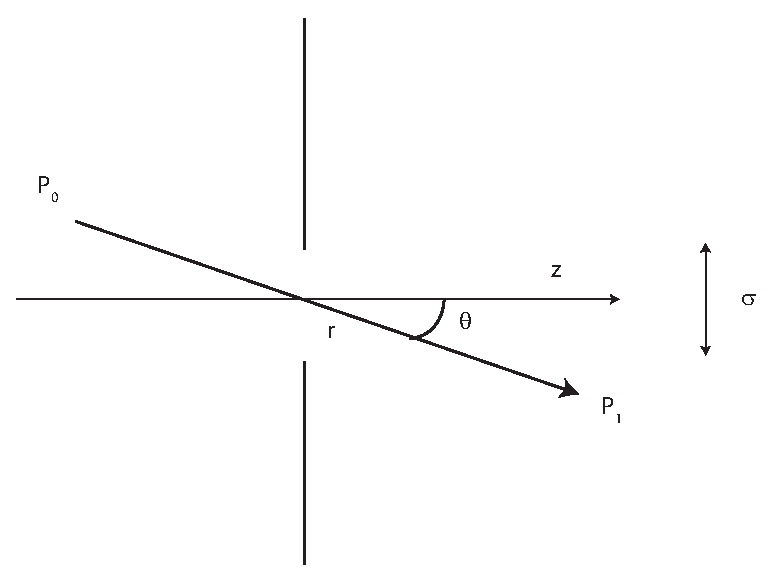
\includegraphics[height=5cm]{RS.eps}
				\end{tabular}
			\end{center}
			\caption{ \label{fig:RS} 
				Geometry of the aperture. }
		\end{figure} 
\subsection{The Fresnel Approximation}
\label{sec:fresnelapprox}
It is possible to approximate the distance of propagation $r$ between $P_0$ and $P_1$ with its Taylor expansion up to the second order:
\begin{equation}
\label{eq:taylor}
r=\sqrt{1+\left(\dfrac{x-\xi}{z}\right)^2+\left(\dfrac{y-\eta}{z}\right)^2}\approx z\left[1+\frac{(1)}{2}\left(\dfrac{x-\xi}{z}\right)^2+\frac{1}{2}\left(\dfrac{y-\eta}{z}\right)^2\right]
\end{equation}
Therefore for large propagation distances, $z\gg x,y$, the diffraction integral becomes:
\begin{equation}
\label{eq:Fresnel}
	U(x,y)=\dfrac{e^{jkz}}{j\lambda z} \int\int_{-\infty}^{\infty}U(\xi,\eta)e^{\frac{jk}{2z}\left[(x-\xi)^2+(y-\eta)^2\right]} d\xi d\eta
\end{equation}
Factorizing the exponential term the disturbance becomes:
\begin{equation}
\label{eq:Fresnel1}
U(x,y)=\dfrac{e^{jkz}}{j\lambda z} e^{j\frac{k}{2z}(x^2+y^2)} \int\int_{-\infty}^{\infty}U(\xi,\eta)e^{\frac{jk}{2z}(\xi^2+\eta^2)}e^{\frac{-jk}{2z}(x\xi+y\eta)} d\xi d\eta
\end{equation}
This can be seen as the Fourier transform of the disturbance before the aperture $U(\xi,\eta)$ multiplied by a quadratic phase factor
 $e^{\frac{jk}{2z}(\xi^2+\eta^2)}$ \cite{goodman2005introduction}.
\section{Free Space Propagation Operator: Fresnel Approximation Approach}
\label{sec:Fresnel}
The first version of the free space propagation operator has been developed using the Fresnel Integral as written in equation \ref{eq:Fresnel1}.
The input disturbance $U(\xi,\eta)$ is considered to be illuminated by monochromatic light with wavelength $\lambda$. As stated in section \ref{sec:fresnelapprox} the Fresnel integral can be seen as the two dimensional Fourier transform of the input field $U(\xi,\eta)$ multiplied by a quadratic phase factor \cite{goodman2005introduction, sypek1995light}. This is going to be very useful from a computational point of view since it can be implemented with a fast The function $U'(\xi,\eta)$ is defined as:
\begin{equation}
	\label{eq:U1}
	U'(\xi,\eta)=U(\xi,\eta)e^{\frac{jk}{2z}(\xi^2+\eta^2)}
\end{equation}
The optical field at the plane $z$ is the product of the Fourier transform of $U'(\xi,\eta)$ with the phase term $e^{\frac{jk}{2z}(x^2+y^2)}$:
\begin{equation}
	\label{eq:FT1}
	U(x,y) = \dfrac{e^{ikz}}{i\lambda z}e^{\frac{ik}{2z}(x^2+y^2)}\mathcal{F}[U'(\xi,\eta)]
\end{equation}
where the spatial frequencies of the Fourier Transform can be correlated with the spatial coordinates $x$ and $y$ by the relation:
\begin{equation}
\label{eq:spacefreq}
\left\{
\begin{array}{l l}
 f_x=\frac{x}{\lambda z} \\
 f_y=\frac{y}{\lambda z}
\end{array} \right.\
\end{equation}
This method is computationally fast since it requires only one Fourier transform, and it is analytically correct. Particular attention should be given to the sampling of the optical fields U and U'. Because of the presence of the Fourier transform the coordinates of the input and output fields are not sampled in the same way, but are scaled by a factor that is proportional to the distance of propagation, as shown in equation \ref{eq:spacefreq} \cite{gonzalez2004digital}. Therefore the input and output planes have different sampling \cite{sypek1995light}.
In addition the multiplicative phase factor:
\begin{equation}
\label{eq:phase2}
e^{\frac{ik}{2z}(\xi^2+\eta^2)}
\end{equation}
presents rapid oscillation of the phase of the optical field for small variations of z, since z is at its denominator \cite{sypek1995light, matsushima2009band}. In order to avoid aliasing the input field requires a large sampling and this is achieved by zero padding the sampling window of the input field, with an increase of the digital resolution of the field. It is known that the computational effort of the FFT algorithm increases with the resolution as $O(n \log n)$, where $n$ is the number of samples of the input field and increasing the sampling resolution of the field \cite{bracewell1965fourier} leads to a long computational time. 
\subsection{Multi-Step Fresnel Propagation Operator}
\label{sec:fresnelmulti}
To overcome the scaling of the field and the large computational time required by the Fresnel propagation integral method a modified method has been developed. 
A multi step approach as the one explained by Sypek \cite{sypek1995light, sypek2009reply} and shown in figure \ref{fig:multistepfig} was used. 
\begin{figure}[h]
	\begin{center}
		\begin{tabular}{c}
				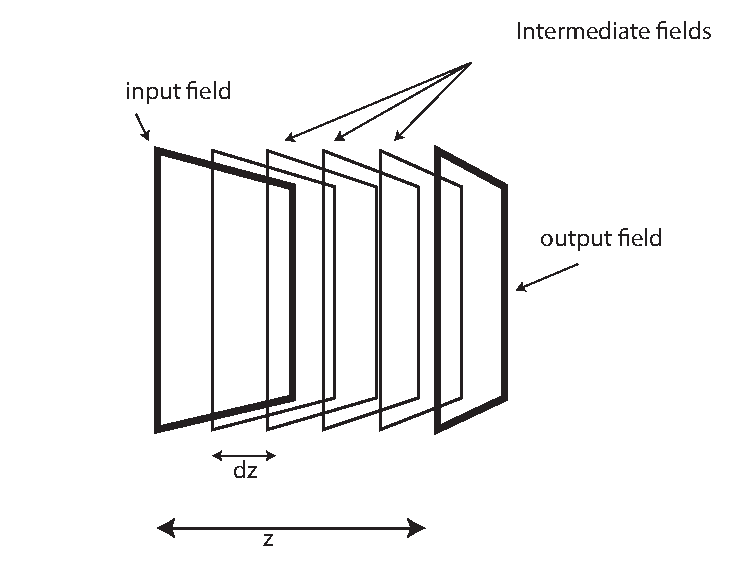
\includegraphics[height=6cm]{multistepfig.eps}
		\end{tabular}
	\end{center}
	\caption{\label{fig:multistepfig} To remove the scaling factor between the input and output fields, a multi step Fresnel approach has been developed. The field is propagated by unit of dz, the minimum distance to keep the sampling the same. } 
	\end{figure}
The reason to adopt the multi-step approach in this project is to remove the scaling factor between the input field and the output field that arise from the Fourier transform as shown in equation \ref{eq:spacefreq}, while Sypek developed a multi step propagation model to minimize the oscillations of the Fourier spectrum and to avoid large zero paddings.\\ In the Fourier domain, an optical field sampled by a $N \times N$ pixels window, and with squared pixels that are $dx$ wide the spatial frequency resolution is \cite{bracewell1965fourier,gonzalez2004digital}:
\begin{equation}
\label{eq:getz1}
df_x=\dfrac{1}{Ndx}
\end{equation}
 Therefore the pixel size in the image plane is according to equations \ref{eq:spacefreq}:
\begin{equation}
\label{eq:pixelsize}
d\xi=d\nu\lambda z
\end{equation} 
where $z$ is the propagation distance and $\lambda$ is the wavelength of the monochromatic wave. The condition to keep the same resolution both in the input field and the output field is:
\begin{equation}
\label{eq:getz}
d\xi=df_x\lambda z=dx
\end{equation}
Substituting equation \ref{eq:getz1} into equation \ref{eq:spacefreq}:
\begin{equation}
\label{eq:getz2}
\dfrac{1}{Ndx}=\frac{dx}{\lambda z}
\end{equation}
Then resolving for z the minimum propagation distance $dz$ to keep the same sampling both in the input and output fields is:
\begin{equation}
\label{eq:getz3}
dz=\frac{W^2}{N\lambda }
\end{equation}
and:
\begin{equation}
	\label{eq:getz4}
	z=\displaystyle\sum_{i=1}^{N} dz_i
\end{equation}
where $W=Ndx$ is the dimension in meters of the input field. Equation \ref{eq:getz3} gives the length of the single step in which the propagation distance $z$ should be divided in order to keep the same resolution.\\ Although the results obtained with this multi-step approach are correct there are some issues. The propagation distance should be a multiple of $dz $, and this is a very significant limitation, especially since in simulating plenoptic systems the distances need to be set precisely. Another issue regards the computational time. With the multi step approach the number of FFT performed increases with the steps, leading to a computational time \textit{N} times larger that the Fresnel Integral method. For these reasons the angular spectrum method as will be discussed in section \ref{sec:angular} has been adopted in all the simulations presented in this work. 
\section {Free Space Propagation Operator: Angular Spectrum of Plane Waves Approach}
\label{sec:angular}
 In the Fourier domain the input disturbance can be seen as formed by a set of plane waves travelling in different directions, the \textit{Angular Spectrum of Plane waves} representation of an optical field. In the next section the propagation operator as and its characteristic transfer function will be defined. Three versions of the angular spectrum operator will be presented, and performances of the three versions will be compared.
\subsection{Angular Spectrum of Plane Waves}
\label{sec:angular 2}
The disturbance $U(x,y;0)$ describing a monochromatic wave incident on a plane \textit{(x,y)} at the \textit{z=0} while travelling along the z direction has a Fourier transform given by:
\begin{equation}
\label{eq:AS1}
A(f_x,f_y;0)=\iint_{-\infty}^{\infty} U(x,y;0)e^{-j2\pi(f_x x+f_y y)}dx dy
\end{equation}
and $U(x,y;0)$ is equal to the inverse Fourier transform of its spectrum:
\begin{equation}
\label{eq:AS2}
U(x,y;0)=\iint_{-\infty}^{\infty} A(f_x,f_y;0)e^{j2\pi(f_x x+f_y y)}df_x df_y
\end{equation}
The physical meaning fo the equation \ref{eq:AS2} is that the disturbance $U(x,y;0)$ can be decomposed in the sum of elemental plane waves propagating in directions given by the wave vector $\overrightarrow{k}$ whose magnitude is $2\pi/\lambda$ and direction is given by its direction cosines $(\alpha,\beta,\gamma)$ \cite{goodman2005introduction,matsushima2009band}.
Dropping the temporal dependence the plane wave is then:
\begin{equation}
\label{eq:AS3}
p(x,y;z)=e^{-j\overrightarrow{k}\cdot\overrightarrow{r}}\\
\end{equation}
where
\begin{equation}
\label{eq:AS4}
 \overrightarrow{r}=x\widehat{i}+y\widehat{j}+z\widehat{k}\\
\end{equation}
and
\begin{equation}
\label{eq:AS5}
 \overrightarrow{k}=\dfrac{2\pi}{\lambda}(\alpha\widehat{i}+\beta\widehat{j}+\gamma\widehat{k})	\\
\end{equation}
The exponential becomes:
\begin{equation}
\label{eq:AS6}
p(x,y;z)=e^{-j\frac{2\pi}{\lambda}(\alpha x+\beta y)}e^{-j\frac{2\pi}{\lambda}(\gamma z)}
\end{equation}
The terms, $\alpha, \beta$ and $\gamma$ are the direction cosines of the wave vector $\overrightarrow{k}$ and they are related as:
\begin{equation}
\label{eq:AS7}
\gamma = \sqrt{1-\alpha^2+\beta^2}
\end{equation}
Therefore the complex exponential function in equation \ref{eq:AS1} can be seen as a plane wave with direction cosines
\begin{equation}
\label{eq:AS8}
\alpha=\lambda f_x, \ \ \beta=\lambda f_y, \ \ \gamma = \sqrt{1-(\lambda f_x)^2+(\lambda f_y)^2}
\end{equation}
The angular spectrum of plane waves of the disturbance $U(x,y;0)$ is the function:
\begin{equation}
\label{eq:AS9}
A\left(\frac{\alpha}{\lambda},\frac{\beta}{\lambda};0\right)=\iint_{-\infty}^{\infty} U(x,y;0)e^{-j2\pi(\frac{\alpha}{\lambda} x+\frac{\beta}{\lambda} y)}dx dy
\end{equation}
After a prorogation of $z$ the disturbance $U(x,y;z)$ can be written in the form of the angular spectrum in analogy with equation \ref{eq:AS2}:
\begin{equation}
\label{eq:AS10}
U(x,y;z)=\iint_{-\infty}^{\infty} A(f_x,f_y;z)e^{j2\pi(f_x x+f_y y)}df_x df_y
\end{equation}
where $f_x=\alpha/\lambda$ and $f_y=\beta/\lambda$.
To be a propagative disturbance, equation \ref{eq:AS10} should satisfy the Helmholtz equation \ref{eq:helmotz}:
\begin{equation}
\label{eq:AS11}
(\nabla^2+k^2)U=0	
\end{equation}
Substituting equation \ref{eq:AS10} into \ref{eq:AS11}:
 \begin{equation}
 \label{eq:AS12}
\dfrac{d^2}{dz^2}A(f_x,f_y;z)+\left(\dfrac{2\pi}{\lambda}\right)[1-(\lambda f_x)^2 + (\lambda f_y)^2 ]A(f_x,f_y;z)=0
 \end{equation}
 A solution of the differential equation \ref{eq:AS12} is:
 \begin{equation}
 \label{eq:AS13}
 A(f_x,f_y;z)=A(f_x,f_y;0)e^{j \frac{2\pi}{\lambda}\sqrt{1-(\lambda f_x)^2+(\lambda f_y)^2}}
 \end{equation}
 The propagative solution is the one where the spatial frequencies satisfy the condition:
 \begin{equation}
 \label{eq:AS14}
 (\lambda f_x)^2+(\lambda f_y)^2<1
 \end{equation}
 in this case the exponential term in equation \ref{eq:AS13} remains complex and the wave can propagate since it is an oscillating term. For the values of spatial frequencies that satisfy the condition:
 \begin{equation}
 \label{eq:AS15}
 (\lambda f_x)^2+(\lambda f_y)^2>1
 \end{equation}
 the exponent in the equation \ref{eq:AS13} becomes real, and the exponential is a decay term. The solution is no longer propagative and waves are called evanescent waves. It is interesting to see how the angular spectrum theory is more complete than the Fresnel approximation since it includes evanescent components too.\\
 Finally, the disturbance after a propagation in z can be expressed as a function of the disturbance $U(x,y;0)$ at the plane z=0:
 \begin{equation}
 \label{eq:AS16}
 U(x,y;z)=\int\int_{-\infty}^{\infty} A(f_x,f_y;0)e^{j \frac{2\pi}{\lambda}\sqrt{1-(\lambda f_x)^2-(\lambda f_y)^2}}e^{j2\pi(f_x x+f_y y)}df_x df_y
 \end{equation}
 The last equation enables a calculation of the output field $U(x,y;z)$ in terms of the input field and the propagation distance, under the approximation of a linear, isotropic, homogeneous and non dispersive medium.\\
 Because of the linearity of the problem, the propagation is considered as a linear system that maps the input disturbance $U(x,y;0)$ into the a new field distribution $U(x,y;z)$\cite{goodman2005introduction}. This linear system is characterized by a transfer function whose bandwidth is limited to the case of the propagative solution of equation \ref{eq:AS12}, excluding the evanescent waves. The angular spectrum of the output field can be rewritten as the product of the angular spectrum of the input field multiplied by the transfer function $H(f_x,f_y)$:
 \begin{equation}
 \label{eq:AS17}
 A(f_x,f_y;z) = A(f_x,f_y;0)\cdot H(f_x,f_y;z)
 \end{equation}
 The propagation is fully described by the transfer function:
 \begin{equation}
 \label{eq:AS18}
H(f_x,f_y;z)=\begin{cases}e^{j \frac{2\pi z}{\lambda}\sqrt{1-(\lambda f_x)^2-(\lambda f_y)^2}} & \quad \text{if } \sqrt{f_x^2+f_y^2}<\frac{1}{\lambda}\\ 0 & \quad \text{otherwise }\\ \end{cases} 
 \end{equation}
 The bandwidth can be represented as a circle in Fourier space. For frequencies smaller than $1/\lambda$ the transfer function introduces a shift in the spatial domain that is responsible for diffraction \cite{goodman2005introduction}.
 Results obtained with the angular spectrum method are similar to the ones obtained with the Fresnel approximation, but no scaling factor between the input and output field is introduced. 
 From a computational point of view, the angular spectrum operator is composed of 3 steps: 
 \begin{enumerate}
 	\item Fourier transform of the input field
 	\item Multiplication of the Fourier transform of the input field with the propagation transfer function in equation \ref{eq:AS18} 
 	\item Inverse Fourier transform of the product at step 2. The resultant field is the output disturbance after the propagation in free space. 
 \end{enumerate}
 The process can be seen in figure \ref{fig:ASflux}
 \begin{figure}[H]
 	\begin{center}
 		\begin{tabular}{c}
 				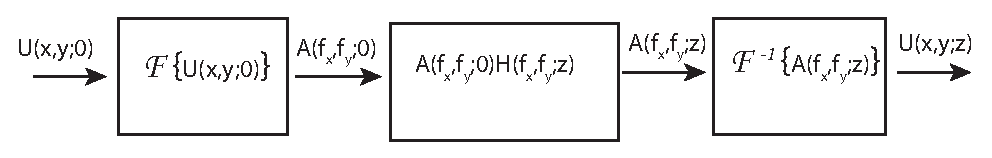
\includegraphics[height=1.5cm]{asflux.eps}
 				\end{tabular}
 		\end{center}
 			\caption{ \label{fig:ASflux} 
 				Structure of the operator free space propagation with the angular spectrum of plane waves method. The initial disturbance $U(x,y;0)$ is transformed into the angular spectrum $A(f_x,f_y;0)$ with a Fourier transform implemented by a FFT algorithm. The angular spectrum is multiplied by the propagation transfer function $H(f_x,f_y)$ and the resultant angular spectrum is inverse transformed into the output disturbance $U(x,y;z)$ }
 \end{figure}
 \subsection{Band Limited Angular Spectrum}
 The transfer function of the propagation in equation \ref{eq:AS18} is a complex exponential oscillating with a frequency depending by the propagation distance $z$. Figure \ref{fig:AStransfer} shows four different profiles of the transfer function for four propagation distances, \textit{1 mm, 2 mm, 10 mm and 20 mm}. Aliasing effects are evident since for a propagation distance of \textit{2 mm}. When the \textit{z} becomes large, the aliasing arises at low spatial frequencies, narrowing the useful bandwidth of the transfer function \cite{matsushima2009band}.
 The transfer function can be rewritten as:
 \begin{equation}
 	\label{eq:BL1}
 	H(f_x,f_y) = e^{j \phi(f_x,f_y)}
 \end{equation}
 where $\phi$ is the oscillating phase term as:
 \begin{equation}
 	\label{eq:BL2}
 	\phi(f_x,f_y)=\dfrac{2\pi}{\lambda}\sqrt{1-\lambda f_x^2-\lambda f_y^2}
 \end{equation}
 \newpage
 \begin{figure}[H]
 	\begin{center}
 		\begin{tabular}{c}
 			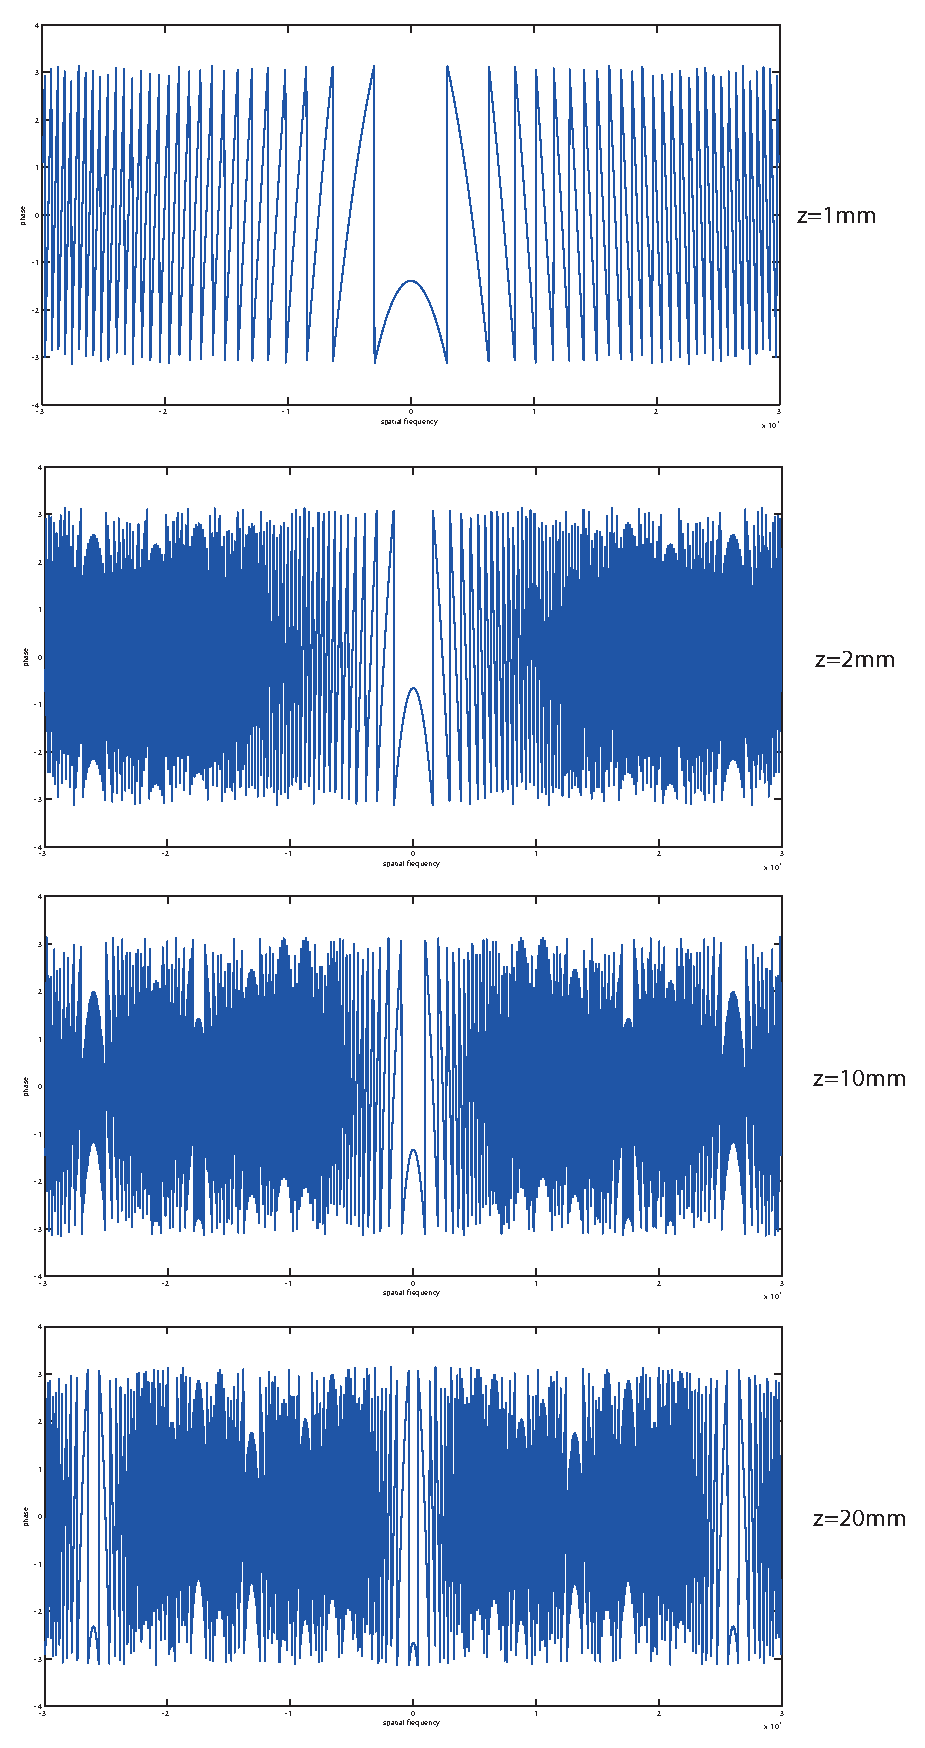
\includegraphics[height=16cm]{phaseH01.eps}
 		\end{tabular}
 	\end{center}
 	\caption 	{ \label{fig:AStransfer} 
 		Cross section along of the phase of the transfer function of the angular spectrum. It is evident how increasing the propagation distance increases the oscillating frequency leading to aliasing. }
 \end{figure}
 \newpage
 Defining the local spatial frequencies of the transfer function \cite{goodman2005introduction,matsushima2009band} as the frequency of the phase oscillation $\nu_x$ and $\nu_y$ along $f_x$ and $f_y$:
 \begin{equation}
 	\label{eq:BL3}
 	\begin{cases} \nu_x=\dfrac{1}{2\pi}\dfrac{\partial}{\partial f_x}\phi(f_x,f_y)\\
 	\\
 	 \nu_y=\dfrac{1}{2\pi}\dfrac{\partial}{\partial f_y}\phi(f_x,f_y)\\ \end{cases}
 \end{equation}
 the local spatial frequencies become:
 \begin{equation}
 \label{eq:BL16}
 \begin{cases} \nu_x=-\dfrac{z}{\lambda}\dfrac{\lambda^2 f_x}{\sqrt{1-(\lambda f_x)^2}}\\
 \\
 \nu_y=-\dfrac{z}{\lambda}\dfrac{\lambda^2 f_y}{\sqrt{1-(\lambda f_y)^2}}\\ \end{cases}
 \end{equation}
 As stated by Matsushima and Shimobaba \cite{matsushima2009band}, if the input optical disturbance is sampled by an $N \times N$ sampling window with pixel size $dx$, the transfer function is sampled by units of spatial frequency equal to $df=1/(N dx)$. To satisfy the Nyquist condition the sampling frequency should be at least the double of the bandwidth of the transfer function. For one direction in the local frequency space:
 \begin{equation}
 \label{eq:BL4}
 \dfrac{1}{df}\geq 2|\nu_x|
 \end{equation}
 Modifying the sampling of the transfer function, and of the input field, can lead to huge sampling windows and long computational times. In addition to that in practical applications the sampling interval is usually fixed. Therefore the condition on the maximum frequency range for which the transfer function is not aliased:
 \begin{equation}
 \label{eq:BL5}
 \dfrac{1}{df_x}\geq 2 z\dfrac{|f_x|}{|\sqrt{(\frac{1}{\lambda^2}+f_x)^2}|}\\ 
 \end{equation}
 Resolving the equation for $|f_x|$ :
 \begin{equation}
 \label{eq:BL6}
 |f_x|\leq\dfrac{1}{\lambda\sqrt{(2df_x z)^2+1}} = f_{max}
 \end{equation}
 Where $f_{max}$ is the maximum frequency of the transfer function without generating errors due to aliasing. Assuming the sampling of the optical field to be the same in both x and y direction the maximum bandwidth for the sampling in $f_y$ is equal to the bandwidth in $f_x $. Therefore:
 \begin{equation}
 \label{eq:BL7}
 \dfrac{1}{df_y}\geq 2|\nu_y|
 \end{equation}
 \begin{equation}
 \label{eq:BL8}
 \dfrac{1}{df_y}\geq 2 z\dfrac{|f_y|}{|\sqrt{(\frac{1}{\lambda^2}+f_y)^2}|}\\ 
 \end{equation}
 \begin{equation}
 \label{eq:BL9}
 |f_y|\leq\dfrac{1}{\lambda\sqrt{(2df_y z)^2+1}} = f_{max}
 \end{equation}
 To avoid aliasing then, the two dimensional transfer function should be limited to a range of frequencies defined by equation \ref{eq:BL8}.
 The expression of the output field will then be:
 \begin{equation}
 \label{eq:BL10}
 U(x,y;z)= \mathcal{F}^{-1}\left[A(f_x,f_y;0)H'(f_x,f_y;z)\right]
 \end{equation}
 where
 \begin{equation}
 \label{eq:BL11}
 H'(f_x,f_y;z)=H(f_x,f_y;z)rect\left(\dfrac{f_x}{f_{max}}\right)rect\left(\dfrac{f_y}{f_{max}}\right)
 \end{equation}
 The MATLAB algorithm to implement the band limitation consists in multiplying the phase term of the propagation transfer function by a phase mask with the shape of a circle function of radius $f_{max}$ in the plane of the spatial frequencies. A circular phase mask has been chosen instead of the rectangular phase mask of equation \ref{eq:BL11} because it follows the geometry of the lens aperture, without introducing new spatial features that could effect the diffraction.\\ The resultant phase of the transfer function is shown in figure \ref{fig:bandlimitedH}, with the bandwidth for three different propagation distances.
 \begin{figure}[H]
 	\begin{center}
 		\begin{tabular}{c}
 				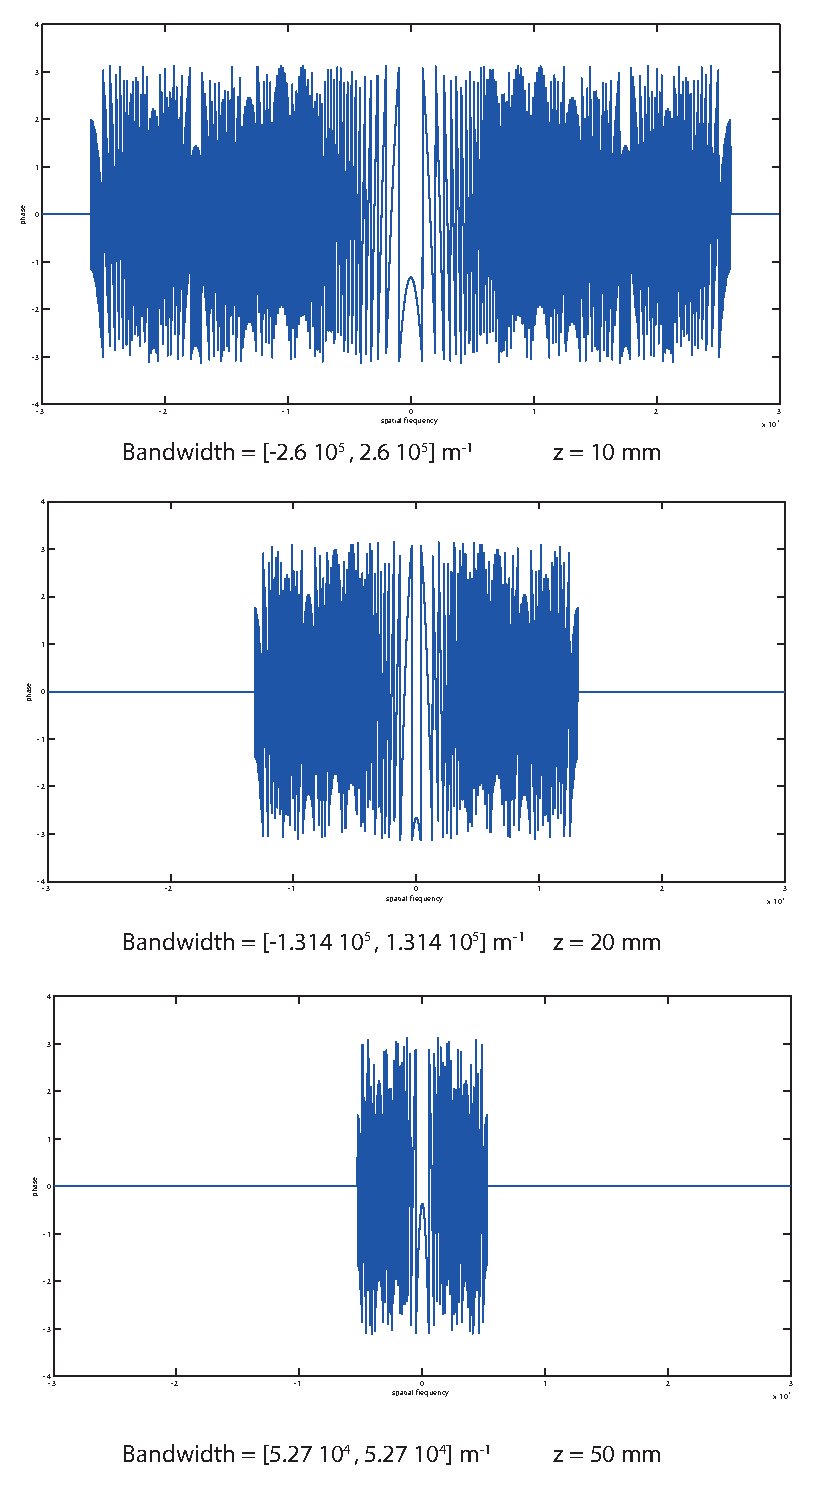
\includegraphics[height=15cm]{phaseHBL.eps}
 		\end{tabular}
 	\end{center}
 	\caption { \label{fig:bandlimitedH} 
 		Bandwidth of the transfer function for three different propagation distances. }
 \end{figure} 
 From a computational point of view the algorithm to implement the band limited angular spectrum method can be summarized in the following steps:
 \begin{enumerate}
		\item Computation of the angular spectrum of the input disturbance via a Fourier transform as shown in equation \ref{eq:AS2}.
		\item Estimation of the maximum bandwidth of the transfer function in order to avoid aliasing error using equation \ref{eq:BL6}.
		\item Multiplication of the phase of the transfer function with a circular phase mask with radius equal to the frequency obtained in the previous step.
		\item Multiplication of the angular spectrum with the band limited transfer function.
		\item Inverse Fourier transform of the product at step 4 
 \end{enumerate}
 The structure of the free space propagation operator implemented by the band limited angular spectrum can be seen in figure \ref{fig:BLAS} 
 \newpage
 \begin{figure}[H]
 	\begin{center}
 		\begin{tabular}{c}
 			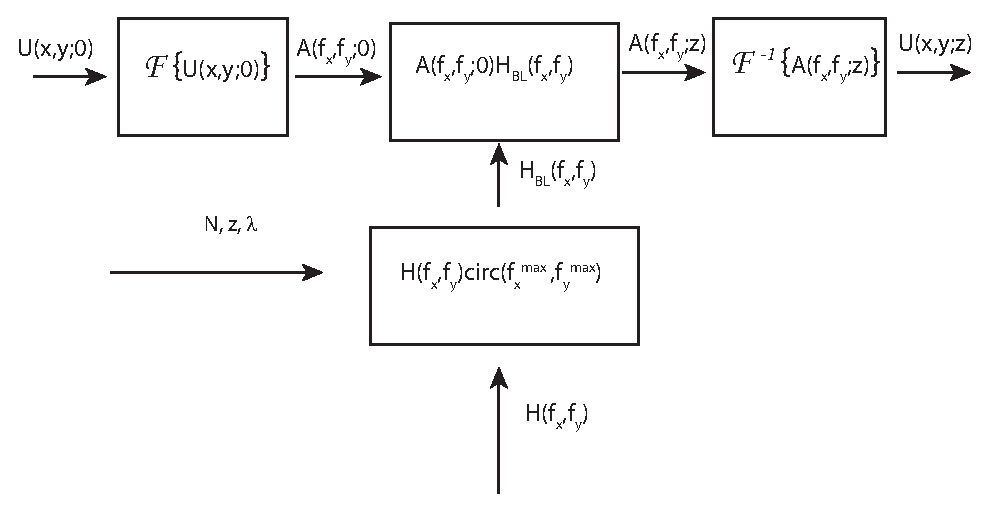
\includegraphics[height=5cm]{asfluxBL.eps}
 		\end{tabular}
 	\end{center}
 	\caption	{ \label{fig:BLAS} 
 		Structure of the operator free space propagation with the angular spectrum of plane waves method in its band limited version. The initial disturbance $U(x,y;0)$ is transformed into the angular spectrum $A(f_x,f_y;0)$ with a Fourier transform implemented by a FFT algorithm. The angular spectrum is multiplied by the propagation transfer function $H(f_x,f_y)$ whose bandwidth has been limited according to equation \ref{eq:BL9}. The bandwidth of the transfer function depends on the sampling of the input field, the wavelength of the light $\lambda$ and the propagation distance.The resultant angular spectrum is inverse transformed into the output disturbance $U(x,y;z)$. \textit{N} is the sampling of thr input field, \textit{z} the propagation distance and $\lambda$ the wavelength. }
 \end{figure} 
 \subsection{Corrected Band Limited Angular Spectrum Method}
 \label{sec:angular3}
 The third method to implement the propagation operator with the angular spectrum is the corrected band limited angular spectrum method. The difference between this method and the band limited angular spectrum method presented in section \ref{sec:angular 2} is that the bandwidth of the transfer function is truncated to the value of the cut-off frequency of the free space propagation in case the Nyquist criterion requires a bandwidth is too narrow.\\
 For long propagation distances the propagation transfer function acts as a low pass filter on the spatial frequency components of the input signal. When its bandwidth is bigger than the cutoff frequency calculated with the band limited method to avoid digital aliasing there is a loss of resolution in the final image. A trade-off should therefore be found between the error due to the aliasing and the error due to the excessive bandwidth limitation. For imaging applications this is not an issue since usually the numerical apertures of the optical elements in the imaging system already limit the band passing from the input field to the output field. However it is useful to estimate the bandwidth of the free space propagation defining the maximum spatial frequency that is transferred from the object plane to the image plane. This value defines the amount of information transferred from the input field to the image plane.\\
 With reference to figure \ref{fig:maxfrequency} for a point in the input field, the range of spatial frequencies that are transferred to the output field are the ones whose direction cosines are contained into the angle that includes the sampling window of the output field. In the cases of the propagation distance much bigger than the sampling window, $z>>W $ like in most of the applications of this simulation toolbox the angle $\theta$ is equal to:
 \begin{equation}
 \label{eq:BL12}
 \theta \simeq\dfrac{W}{z}
 \end{equation}
 \begin{figure}[h]
 	\begin{center}
 		\begin{tabular}{c}
 				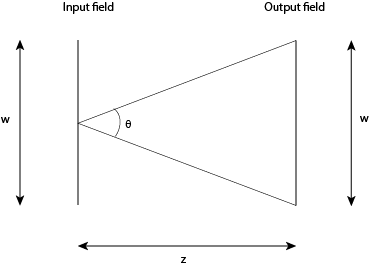
\includegraphics[height=7cm]{cutofffrequency.png}
 		\end{tabular}
 	\end{center}
 	\caption	{ \label{fig:maxfrequency} 
 		The maximum spatial frequency is linked to the dimension of the sampling window of the output field $w$ and the propagation distance $z$ }
 \end{figure} 
 The link between the direction cosine and the spatial frequency is, according to equation \ref{eq:AS8}
 \begin{equation}
 \label{eq:BL13}
 \theta=\lambda f_{cutoff},
 \end{equation}
 The cutoff frequency of a field sampled by a sampling window $W$ and after a propagation distance of $z$ is defined as:
 \begin{equation}
 	\label{eq:BL14}
 	\nu_{cutoff}=\dfrac{W}{\lambda z}
 \end{equation}
 Therefore the bandwidth of the transfer function should be bigger than $\nu_{cutoff}$ in order not to introduce error in the reconstruction of the diffraction pattern due to loss in resolution.
 \begin{equation}
 \label{eq:BL15}
 f_{max}\geq\nu_{cutoff}
 \end{equation}
 If the propagation distance limits the bandwidth of the output field too much, the transfer function can be improved by increasing the sampling of the input field. This condition is equal to having a smaller pixel size. Dealing with bigger sampling windows however increases the computational effort. 
 \subsection{Performances of the Angular Spectrum Methods}
 \label{sec:perfAS}
 To evaluate the differences in resolution of the three variants of the angular spectrum methods, Normal Angular spectrum (AS), Band Limited angular spectrum (BL), and Corrected Band Limited Angular Spectrum (CBL), a simulation has been implemented consisting of a free space propagation of an input field with a circular pupil of diameter 5 mm, sampled with a resolution of 3000 $\times$ 3000 pixels with a sampling window of 1 cm. The propagation distances \textit{z} varied from 1 m to 10 m.\\ 
 Results are shown in figure \ref{fig:methods} where the cross section of the diffraction patterns are shown. 
 The BL method shown in the central column gives smooth diffraction patterns. Increasing the propagation distance however leads to the intensity profile losing part of the information because of the excessive low pass filtering on the propagation transfer function, leading the complete loss of the diffraction fringes. A comparison with the AS can be seen in figure \ref{fig:methods}, where the diffraction fringes are presents with the superimposition of the noise due to aliasing in the transfer function sampling. This affects the resolution of the diffraction pattern and the signal to noise ratio (SNR) drops with \textit{z} as shown in figure \ref{fig:SNR1}.The CBL method gives a good noise reduction without losing the original signal shape as explained in section \ref{sec:angular3} and as it is shown in figure \ref{fig:methods} on the far right column. Fringes are clearly present in the diffraction pattern even for large propagation distances and the noise is removed. \\
 In figure figure \ref{fig:SNR1} the SNR of the diffraction patterns in figure \ref{fig:methods} is plotted as a function of the propagation distance for the three examined cases. The BL method gives a better SNR especially for short propagation distances, where the bandwidth of the transfer function is not low pass filtering the signal yet, but only avoiding the aliasing. Its values remains in general above the SNR of the CBL method (almost 15dB), even in the case of large propagation distances. This is due to the excessive smoothing action that leads to the loss of resolution. On the other hand without any bandwidth limitation, AS, green line, the aliasing generated noise becomes dominant for long propagation distances and the SNR approaches the 0 dB value. The best results in terms of resolution and noise reduction are given by the corrected BL method where the information on the diffraction is entirely kept. 
 \begin{figure}[h]
 	\begin{center}
 		\begin{tabular}{c}
 			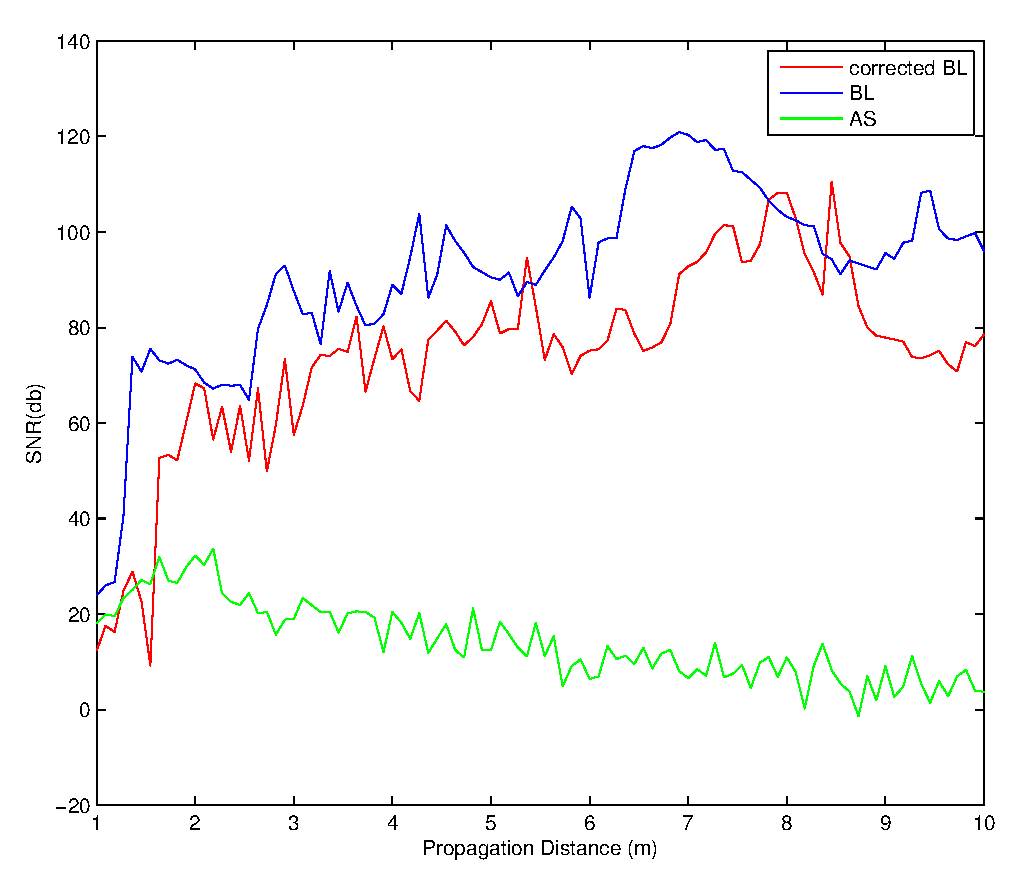
\includegraphics[height=12cm]{SNR_com.eps}
 		\end{tabular}
 	\end{center}
 	\caption	{ \label{fig:SNR1} 
 		Comparison between the Signal to Noise ratio (SNR) as a function of the propagation distance for the three propagation methods seen in section \ref{sec:angular 2}. The BL and the corrected BL methods improve the SNR, that instead drops as the propagation distance increases when the AS method is used. }
 \end{figure} 
  \begin{figure}[H]
  	\begin{center}
  		\begin{tabular}{c}
  			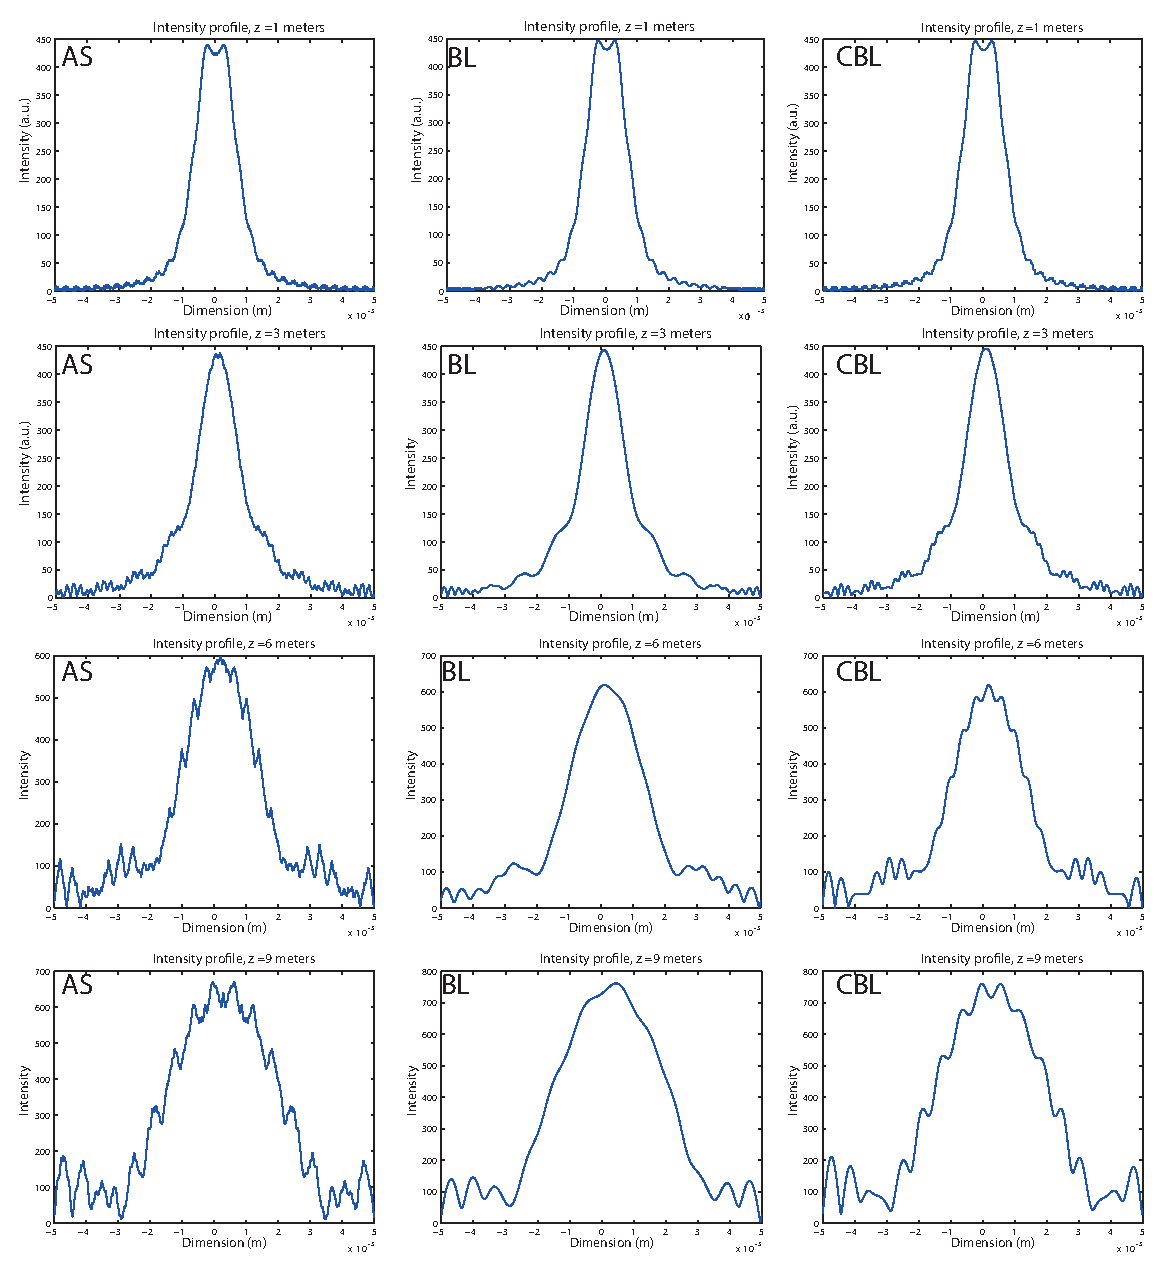
\includegraphics[height=15cm]{methods1.eps}
  		\end{tabular}
  	\end{center}
  	\caption{ \label{fig:methods} 
  		Comparison of the performances of the three angular spectrum propagation operator. On the left column are shown diffraction pattern cross section obtained using the angular spectrum method (AS). In the central column the pattern for the same propagation distances have been obtained using the band limited method (BL) and in the right column the same patterns have been obtained using the correct band limited method (corrected BL). }
  \end{figure}
\section{Thin Lens Operator}
\label{sec:lens}
This section will describe how the thin lens operator has been designed and implemented in the simulation toolbox, following the method described in Goodman \cite{goodman2005introduction}.
A lens is composed of a material with a refractive index different form the one of air, that causes the propagation velocity of the optical field to drop. In the approximation of a thin lens, the translation of the ray of light inside the lens is negligible and if a ray enters the lens at the coordinate $(x,y)$ on one face, it exits at the same coordinates at the other side. A thin lens delays and incident wave-front by an amount proportional to its thickness. These delay can be modelled introducing a phase factor to the incident field. 
The thickness of the lens, $\Delta(x,y)$, is a function of the coordinates \textit{(x,y)} as shown in figure \ref{fig:thick}, where $\Delta_0$ is the lens maximum thickness at the coordinates $(0,0)$.
\begin{figure}[h]
	\begin{center}
		\begin{tabular}{c}
			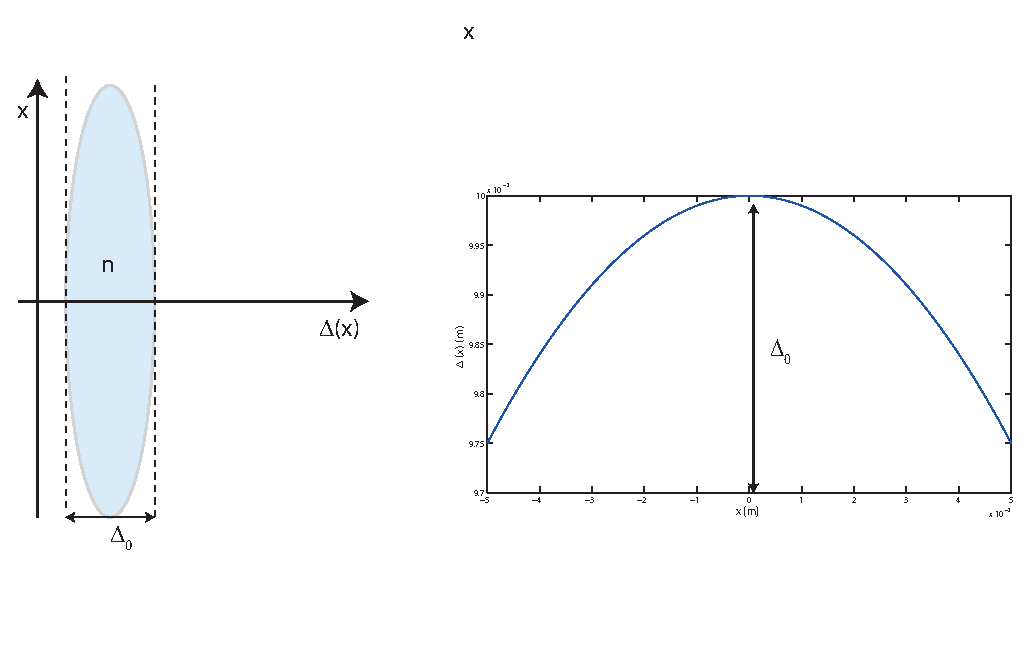
\includegraphics[height=5cm]{lens1.eps}
		\end{tabular}
	\end{center}
	\caption{ \label{fig:thick} 
	Thickness of a lens as a function of position along x coordinate. It can be defined in the same way along the y coordinate}
\end{figure} 
The phase delay introduced by the lens is proportional to its thickness:
\begin{equation}
\label{eq:phase}
	\phi(x,y)=kn\Delta(x,y)+k[\Delta_0-\Delta(x,y)]
\end{equation} 	
where $n$ is the refractive index of the lens material and $k=2\pi/\lambda$ is the wave number. With reference to figure \ref{fig:thick} the quantity
\begin{math}
	kn\Delta(x,y)
\end{math}
is the phase delay introduced by the different material of the lens, and 
\begin{math}
	k[\Delta_0-\Delta(x,y)]
\end{math}
is the phase delay introduced by the free space propagation between the two planes represented with dashed line.
This phase delay can be seen as a multiplicative phase term defined as:
\begin{equation}
\label{eq:delay}
	t_{lens}=\exp[jk\Delta_0]exp[jk(n-1)\Delta(x,y)]
\end{equation}
The complex field 
\begin{math}
	U'(x,y)
\end{math}
immediately after the lens is therefore given by the product of the field entering the lens 
\begin{math}
	U_0(x,y)
\end{math} 
with the phase delay in equation \ref{eq:delay}.
\begin{equation}
\label{eq:disturbance}
	U'(x,y)=t_{lens}(x,y)U_0(x,y)
\end{equation}
The sign convention used in the following derivation for a ray of light travelling form left to right is: 
\begin{itemize}
	\item any convex surface encountered has positive radius of curvature
	\item any concave surface encountered had negative radius of curvature
\end{itemize}
The lens can be split into three elements such that the total thickness function is the sum of three functions:
\begin{figure}[h]
	\begin{center}
		\begin{tabular}{c}
				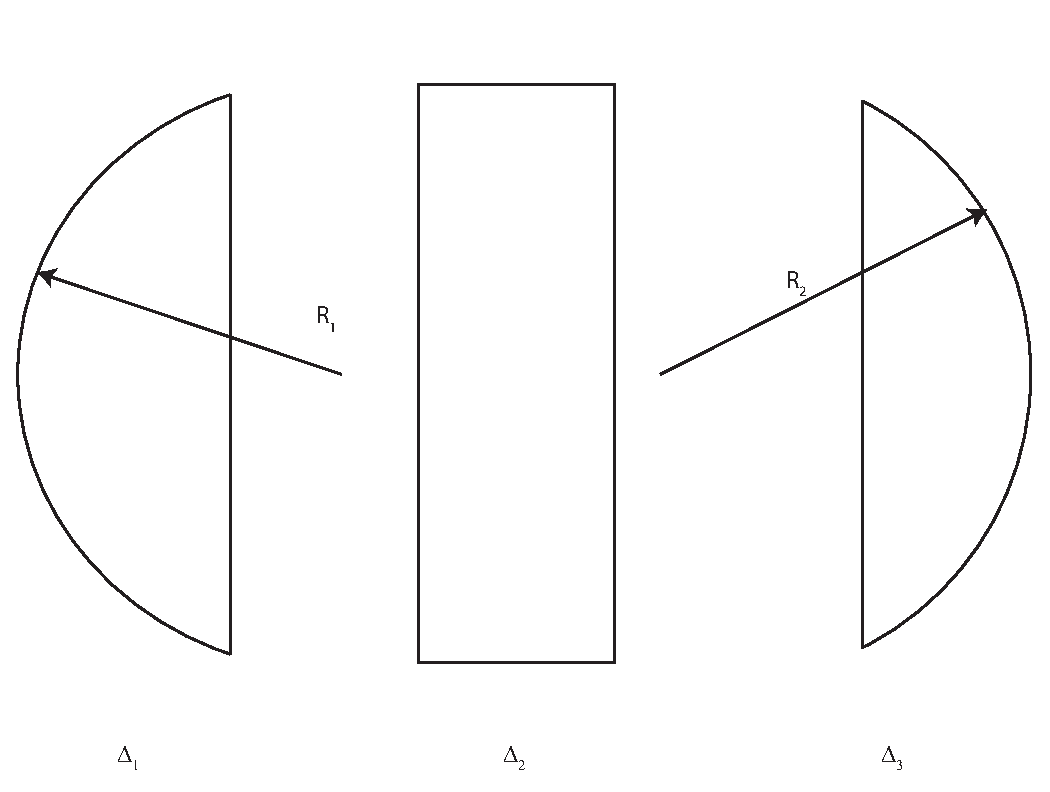
\includegraphics[height=5cm]{lens2.eps}
		\end{tabular}
	\end{center}
	\caption{ \label{fig:split} 
		The thickness function can be decomposed into the sum of three contributions. }
\end{figure} 
From figure \ref{fig:split}:
\begin{equation}
\label{eq:split}
	\Delta(x,y)=\Delta_1(x,y)+\Delta_2(x,y)+\Delta_3(x,y)
\end{equation}
Where the three components of the thickness are:
\begin{equation}
\label{eq:delta1}
\Delta_1(x,y)=\Delta_{01}(x,y)-R_1\bigg(1-\sqrt{1-\frac{x^2+y^2}{R_1^2}}\bigg)
\end{equation}
\\
\begin{equation}
\label{eq:delta2}
\Delta_2(x,y)=\Delta_{02}
\end{equation}
\\
\begin{equation}
\label{eq:delta3}
\Delta_3(x,y)=\Delta_{03}(x,y)-R_2\bigg(1-\sqrt{1-\frac{x^2+y^2}{R_2^2}}\bigg)
\end{equation}
\\

\begin{math}
	R_1>0
\end{math}
and
\begin{math}
	R_2<0
\end{math}
are respectively the radius of curvature of the right-hand surface and the radius of curvature of the left-hand side of the lens surface.
Then total thickness function is given by:
\begin{equation}
\label{eq:delta_sum}
	\Delta(x,y)=\Delta_0(x,y)-R_1\bigg(1-\sqrt{1-\frac{x^2+y^2}{R_1^2}})+R_2(1-\sqrt{1-\frac{x^2+y^2}{R_2^2}}\bigg)
\end{equation}
where $\Delta_0$ is:
\begin{math}
	\Delta_0=\Delta_{01}+\Delta_{02}+\Delta_{03}
\end{math}.
In the paraxial approximation it is possible to approximate $\Delta(x,y)$ with its first element of the Taylor series:
\begin{equation}
\label{eq:approx1}
\sqrt{1-\frac{x^2+y^2}{R_1^2}}\approx 1-\frac{x^2+y^2}{R_1^2}
\end{equation}
\begin{equation}
\label{eq:approx2}
\sqrt{1-\frac{x^2+y^2}{R_2^2}}\approx 1-\frac{x^2+y^2}{R_2^2}
\end{equation}
 Substituting \ref{eq:approx1} and \ref{eq:approx2} into equation \ref{eq:delta_sum}:
 \begin{equation}
 \label{eq:approx3}
 \Delta(x,y)=\Delta_0(x,y)-\frac{x^2+y^2}{2}\bigg(\frac{1}{R_1}+\frac{1}{R_2}\bigg)
 \end{equation}
and substituting \ref{eq:approx3} into equation \ref{eq:phase} the result is the expression of the phase shift in the exponential form:
 \begin{equation}
 \label{eq:expon}
 t_{lens}(x,y)=\exp[jkn\Delta_0]exp[-jk(n-1)\frac{x^2+y^2}{2} \bigg(\frac{1}{R_1}+\frac{1}{R_2}\bigg)]
 \end{equation}
 The focal length of the lens $f$ is the quantity containing the information on the physical properties of the lens and it is defined as:
	\begin{equation}
 \label{eq:focal}
 \frac{1}{f} \equiv(n-1) \bigg(\frac{1}{R_1}+\frac{1}{R_2}\bigg)
	\end{equation}
 Finally after dropping the constant phase factor the effects of a thin lens under paraxial approximation as a quadratic phase transformation are described by equation \ref{eq:lens1}:
 \begin{equation}
 	\label{eq:lens1}
 	t_{lens}(x,y)=\exp[-j\frac{k}{2f}(x^2+y^2)]
 \end{equation}
 This equation can represent the effects of any lens, since the sign of $f$ will define whether the lens is positive or negative.
 The physical meaning of this expression can be understood through figure \ref{fig:lensmeaning}.
	\begin{figure}[h]
		\begin{center}
			\begin{tabular}{c}
					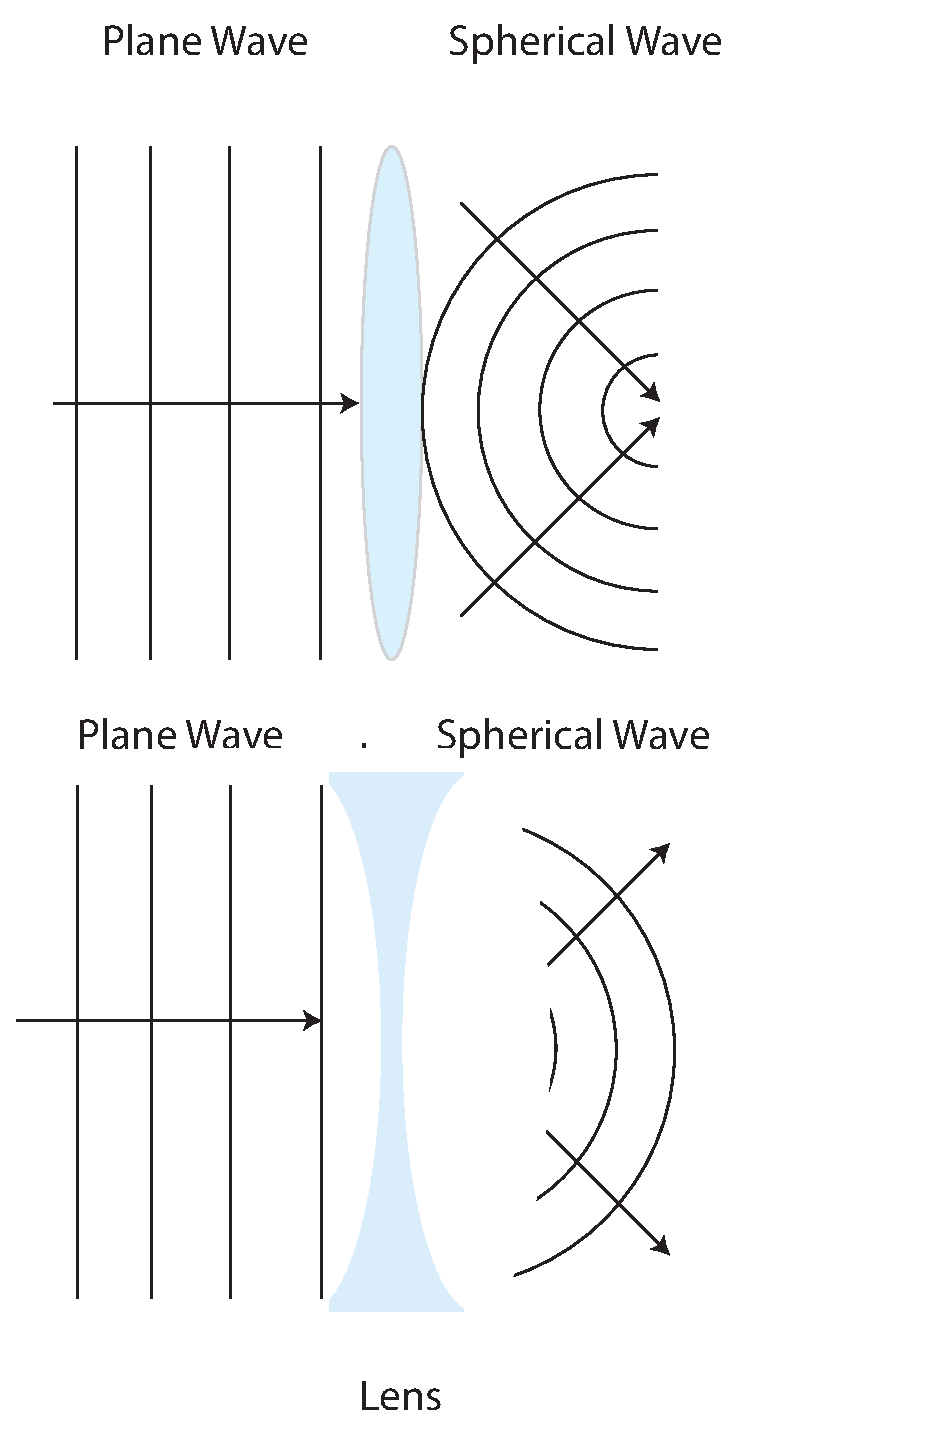
\includegraphics[height=7cm]{lens3.eps}
			\end{tabular}
		\end{center}
		\caption{ \label{fig:lensmeaning} 
			A thin lens converts a plane wave into a spherical wave. }
	\end{figure} 
	When a plane wave represented by the complex field $U(x,y)$ is normally incident on the lens, according to equation \ref{eq:disturbance}, the field leaving of the lens will be:
	\begin{equation}
	\label{eq:disturbance2}
		U'(x,y)=\exp[-j\frac{k}{2f}(x^2+y^2)]
	\end{equation}
	The thin lens is introducing a phase term on the incident field, and the resulting field is a quadratic approximation of a spherical wave. Figure \ref{fig:lensmeaning} shows that when $f$ is positive, the wave is converging towards a point on the optical axis at distance $f$ from the lens. If $f$ is negative the wave is diverging from a point on the optical axis placed at a distance $f$ in front of the lens. The lens therefore transforms a plane wave into a spherical wave. 
	The operator thin lens is defined as the product of the quadratic transformation in equation \ref{eq:lens1} with a function describing the aperture of the lens, called pupil $P(x,y)$ :
	\begin{equation}
	\label{eq:lesop}
		L(x,y)=P(x,y)\exp[-j\frac{k}{2f}(x^2+y^2)]
	\end{equation}
	where the pupil function is defined as:
	\begin{equation}
	\label{eq:pupil}
	 P(x,y) = \left\{
		\begin{array}{l l}
		1 & \quad \sqrt{x^2+y^2}<r \\
		0 & \quad \text{elsewhere}
		\end{array} \right.\
	\end{equation}
	where $r$ is the radius of the lens aperture.
	\subsection{Aliasing in Phase Sampling}
	The quadratic phase factor of the thin lens operator is a complex function whose modulus is constant and equal to unity, and its argument is an oscillating function in the interval $(0,2\pi]$. The argument of the phase factor is shown in figure \ref{fig:argument}
	\begin{figure}[H]
		\begin{center}
			\begin{tabular}{c}
					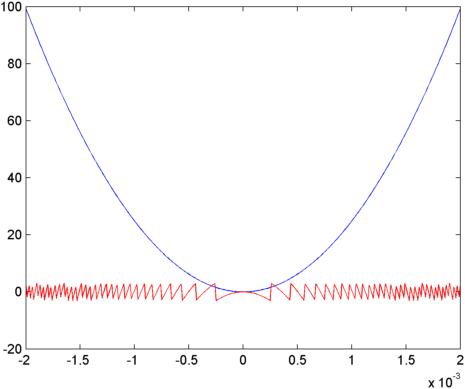
\includegraphics[height=7cm]{C:/Users/Massimo/Documents/Thesis/figures/figurephase.png}
			\end{tabular}
		\end{center}
		\caption{ \label{fig:argument} 
			Phase profile of a computer generated lens. The blue line shows the quadratic phase term and the red line shows the same phase term wrapped every $2\pi$. This wrapping is the source of the aliasing. }
	\end{figure} 
The parabolic phase profile gets wrapped since the argument of a complex function varies between $0$ and $2\pi$. This wrapping of the phase can cause aliasing as the distance from the centre of the lens increases. For high values of $x$ and $y$, the quadratic term becomes too steep and the frequency of oscillation between $0$ and $2\pi$ of the phase factor might become too high to be correctly sampled. With analogy of what has been said in section \ref{sec:angular}, for a parabolic phase profile:
	\begin{equation}
		\label{eq:parabolic}
		\phi(x,y)=\dfrac{k}{2f}(x^2+y^2)
	\end{equation} 
The instantaneous frequencies of the phase $\nu_x$, $\nu_y$ in $x$ and $y$ respectively are defined as:
	 
\begin{equation}
\label{eq:localfreq}
\left\{
\begin{array}{l l}
\nu_x=\dfrac{1}{2\pi}\dfrac{\partial\phi}{\partial x}=\dfrac{1}{2\pi}\dfrac{k}{ f}x\\
\\
\nu_y=\dfrac{1}{2\pi}\dfrac{\partial\phi}{\partial y}=\dfrac{1}{2\pi}\dfrac{k}{ f}y
\end{array} \right.\
\end{equation}
In order to recover all the components of a periodic signal, the sampling frequency should be at least twice the bandwidth of the signal. According to the Nyquist criterion:
\begin{equation}
\label{eq:nyquist}
	f_{Nyquist}=2\nu_{max}
\end{equation} 
The maximum instantaneous frequency $\nu_{max}$ of the phase factor is the one that correspond to the edge of the lens. For brevity the one dimensional case along the $x$ direction is considered, but the conclusions are valid for the $y$ direction because of the rotational symmetry of the pupil function in equation \ref{eq:pupil}. In this case $x_{max}=y_{max}=r$ where $r$ is the radius of the pupil function.
Defining the pixel size $\Delta x$ along $x $, and assuming the pixels as square, so that the sampling frequency $1/\Delta x$ is the same along both axis, the Nyquist condition to avoid aliasing is:
\begin{equation}
	\label{eq:Nyx}
	\dfrac{1}{\Delta x}\geq \dfrac{1}{2\pi}\dfrac{k}{f}x_{max}
\end{equation}
Since in general the sampling rate cannot be modified because of the fixed pixel size of the sensor this expression leads to a condition for the radius of the pupil function:
\begin{equation}
\label{eq:radius_cond}
	r=x_{max}\leq \frac{2\pi f}{k \Delta x}
\end{equation}
Substituting $k=\frac{2\pi}{\lambda}$ into \ref{eq:radius_cond}:
\begin{equation}
\label{eq:radius_cond1}
r\leq \frac{\lambda f}{\Delta x}
\end{equation}
The more powerful the lens, $f$ will have a smaller value and hence the aperture should be smaller.
Therefore, in order to achieve a desired aperture size in equation \ref{eq:radius_cond1}, the focal length must be such that:
\begin{equation}
	\label{eq:focalcond}
	f\geq\frac{r\Delta x }{\lambda}
\end{equation}
and given that the digital resolution of a lens with aperture equal to $2r$ is given by:
\begin{equation}
\label{eq:resolution}
N=\frac{2r}{\Delta x}
\end{equation}
then the minimum resolution of a lens of radius $r$ and focal length $f$ is:
\begin{equation}
	\label{eq:rescond}
	N\geq\frac{2r^2}{f \lambda} 
\end{equation}
Applying these conditions will assure that no aliasing will be introduced by the lens operator.
 \section{Comparison between the Free Space Propagation Operators}
 \label{sec:comp}
	 In this section the differences in performance between the Fresnel approximation and the angular spectrum of plane waves approach will be shown with particular attention to the computational time required by the different methods, the optical resolution and the error. Results will be used to evaluate the characteristic of the different propagation operators. These results differ from the ones obtained in section \ref{sec:perfAS} since the simulations in this case involve the whole imaging system including the lens and not only the free space propagation.
	 \subsection{Description of the System}
	 \label{sec:system}
	 The system simulated is a simple imaging system composed of a single lens with focal length $f=158mm$, in a \textit{2f} configuration, as shown in figure \ref{fig:2f}. The field of view is a square of $1cm \times 1cm$, and the resolution of the input field is $2000 \times 2000$ pixels. The aperture of the lens is $D=5mm$ and its f number, defined as:
	 \begin{equation}
	 \label{eq:fnum}
		F_{\#}=\dfrac{z}{D}
	 \end{equation}
	 is equal to $F_{\#}=63$, where z is the distance from the lens to the image plane, that in a 2f configuration is equal to $z=2f=316mm$.
	 \begin{figure}[h]
	 	\begin{center}
	 		\begin{tabular}{c}
	 			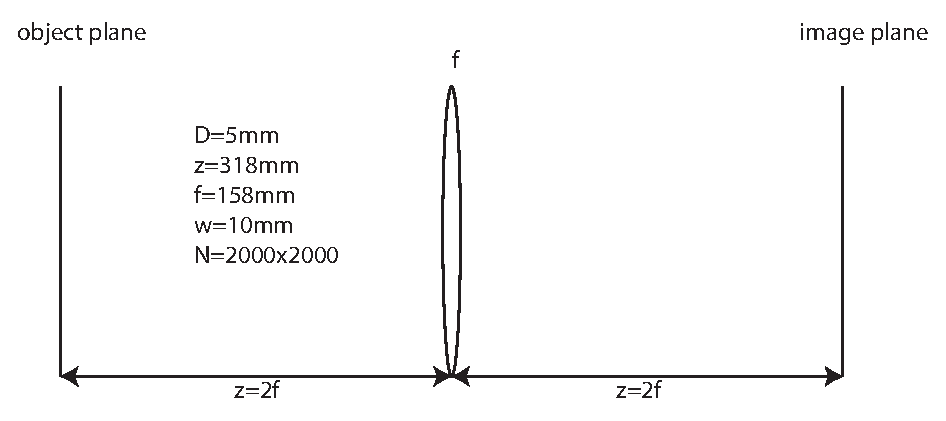
\includegraphics[height=5cm]{C:/Users/Massimo/Documents/Thesis/2f.eps}
	 		\end{tabular}
	 	\end{center}
	 	\caption{ \label{fig:2f} 
	 		Schematic of the 2f system simulated. f is the focal lenght, z the propagation distances, D is the aperture of the lens, w the field of view and N the sampling resolution. }
	 \end{figure} 
	 The optical cut-off frequency of this system is given by the relation \cite{goodman2005introduction}:
	 \begin{equation}
	 \label{eq:cutoff}
	 \nu_c=\dfrac{1}{\lambda F_{\#}}
	 \end{equation} 
	 The object was illuminated with monochromatic light of wavelength $\lambda=633nm$, $\nu_c=2.5\cdot10^4 cycles/m$.
	 \subsection{Image of a Point Source}
	 The first experiment simulated is the image of a point source, realized with a pinhole of $10 \mu m$ of diameter placed at the object plane indicated in figure \ref{fig:2f}. The image has been taken using four different methods to propagate the light into the system. Those are:
	 \begin{itemize}
	 	\item Multi step Fresnel method (MSF), section\ref{sec:fresnelmulti}
	 	\item Angular spectrum method (AS), section \ref{sec:angular}
	 	\item Band Limited Angular Spectrum method (BL), section \ref{sec:angular 2}
	 	\item corrected Band Limited Angular Spectrum method (CBL), section \ref{sec:angular3}
	 		 \end{itemize}
The impulse response for a point source as input will be computed using each of these methods.\\
 The sequence of operators used to simulate the system is shown in figure \ref{fig:sequence2} \\
	 \begin{figure}[H]
	 	\begin{center}
	 		\begin{tabular}{c}
	 			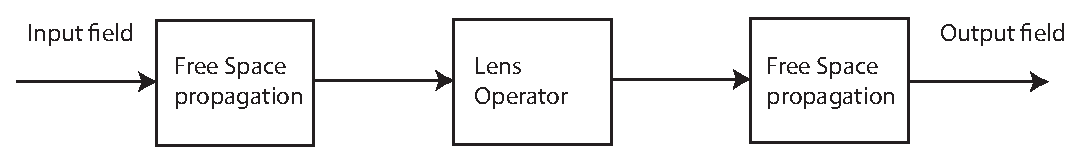
\includegraphics[height=1.8cm]{C:/Users/Massimo/Documents/Thesis/imagesystem.eps}
	 		\end{tabular}
	 	\end{center}
	 	\caption{ \label{fig:sequence2} 
	 		Operator sequence for the 2f system. }
	 \end{figure} 
	 
	In the assumption of having a lens with a circular aperture and no aberrations, the impulse response of an optical system is an Airy Disk, that is the Fourier transform of the pupil of the system at the image plane. The fact that the theoretical output of the experiment is well known allows to determine the quality of the simulation tools.
	In addition to that, the Fourier transform of the impulse response of an optical system gives information on the frequencies content of the image, hence the band pass of the imaging system and its quality. 
	Figure \ref{fig:resultspoint11} shows the sensor image at the image plane together with intensity profiles of the image.
	\newpage
	 \begin{figure}[H]
	 	\begin{center}
	 		\begin{tabular}{c}
	 			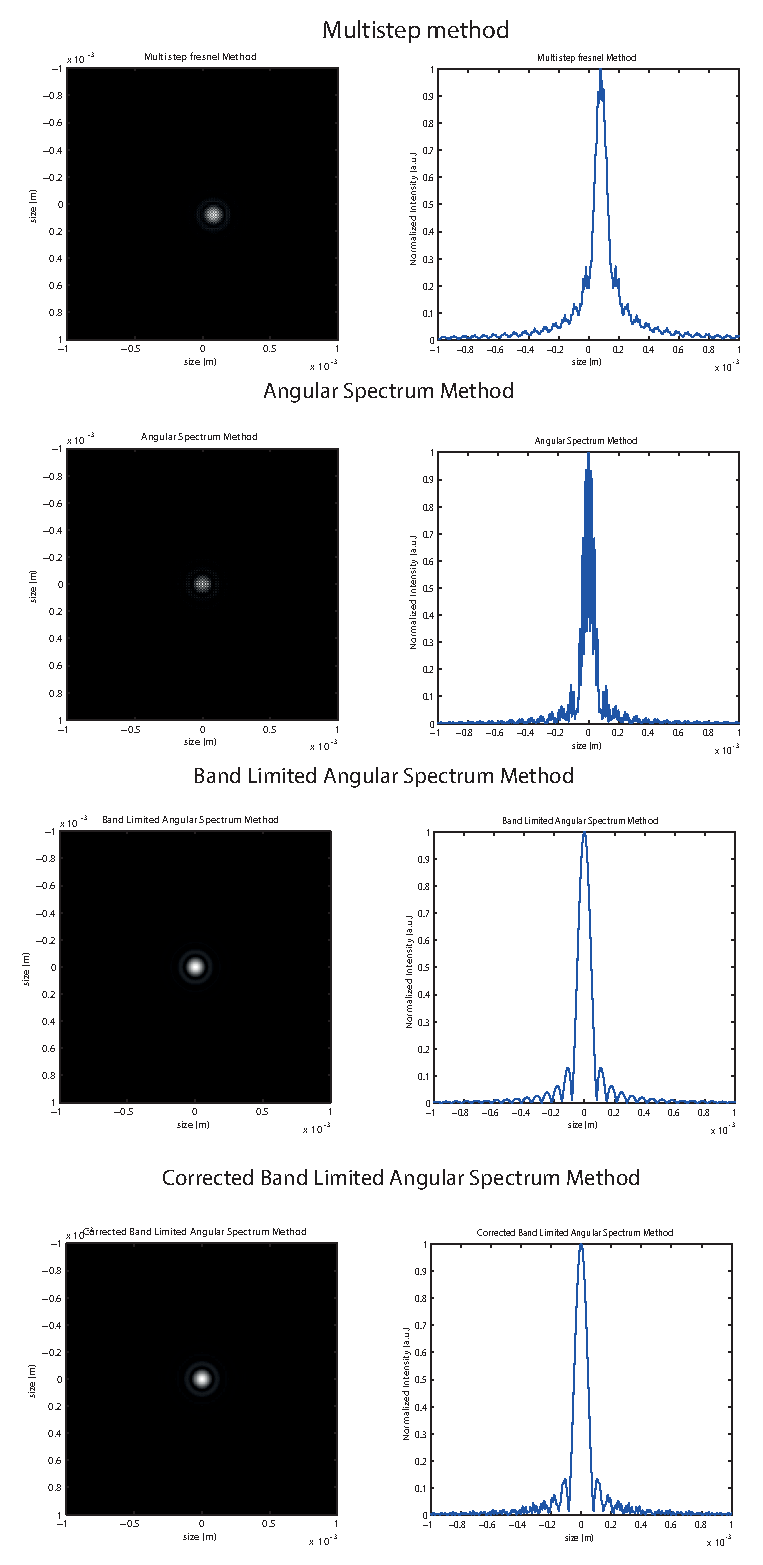
\includegraphics[height=15cm]{C:/Users/Massimo/Documents/Thesis/methodspoint1.eps}
	 		\end{tabular}
	 	\end{center}
	 	\caption{ \label{fig:resultspoint11} 
	 		From top to Bottom: Image and intensity cross section of a point source according to multi step method, angular spectrum method, band limited angular spectrum method and corrected band limited angular spectrum method. }
	 \end{figure} 
	From figure \ref{fig:resultspoint11} it can be seen that in the case of the MSF method the cross section of the impulse response does not go to zero because if additive background noise. The response of the AS method has a high frequency noise components superimposed to the diffraction pattern while the BL method reduces the noise due to aliasing of the transfer function in the AS case as can be seen comparing the two cross sections. Both the BL and the CBL methods present no background noise and in the high frequency noise is reduced with respect to the AS case. Another parameter to evaluate the accuracy of these methods is the position of the Airy disk first minimum. It is given by \cite{goodman2005introduction,pedrotti1993introduction}:
	 \begin{equation}
	 \label{eq:airy}
	 x_{min}=1.22\dfrac{\lambda z}{D}
	 \end{equation}
	 where $D$ is the aperture of the lens. According to the values in section \ref{sec:system} the Airy disk should have a its first minimum at $x_{min}=67 \mu m$.
	 Without considering the MSF case that is too noisy and does not present zeros, the position of the first minimum is the other cases are:\\
	 \begin{center}
	 \begin{tabular}{ l | r }
	 	
	 	\hline			
	 	AS & 67.5 $\mu m$ \\
	 	BL & 77.5 $\mu m$ \\
	 	CBL & 77.5 $\mu m$ \\
	 	\hline 
	 		\end{tabular}
	\end{center}
	As expected for both the band limited angular spectrum methods (BL and CBL) the Airy Disk is slightly wider due to the low pass filtering action that transfer function has undergone. However noise is reduced with the band limitation as shown in figure
	 \ref{fig:resultspoint11}.
	 To better understand how the resolution changes with the different methods, it is worth to have a look at the Fourier transform of the images shown in figure \ref{fig:resultspoint11}. The Fourier transform of the impulse response of a system give its frequency response. The shape of the frequency response gives information about how the frequency components of the input signal are modulated and transferred to the output signal. When this function goes to zero the correspondent frequency value is called the cutoff frequency. For frequencies higher than the cutoff frequency, all the information included in the input signal is lost. Results are shown in figure \ref{fig:resultspoint2}. The graphs are symmetric with respect to the zero frequency, therefore only the positive frequencies are shown.
	 
	 \begin{figure}[h]
	 	\begin{center}
	 		\begin{tabular}{c}
	 			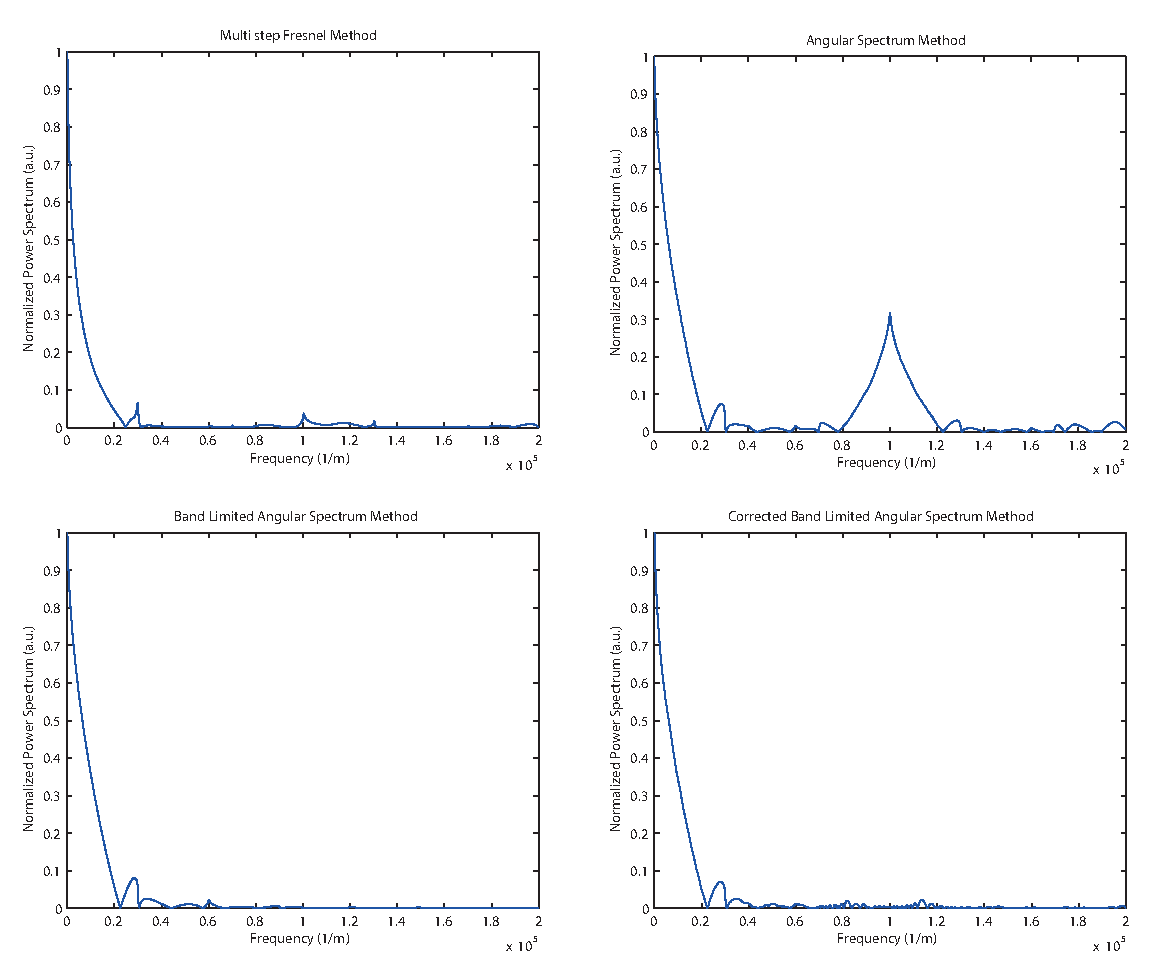
\includegraphics[height=8cm]{C:/Users/Massimo/Documents/Thesis/MTF.eps}
	 		\end{tabular}
	 	\end{center}
	 	\caption{ \label{fig:resultspoint2} 
	 		From top left to bottom right: Power spectrum of the image of a point source obtained with the MSF method, the AS method, the BL method and the CBL method . }
	 \end{figure} 
	From a comparison of the power spectra in figure \ref{fig:resultspoint2} it is possible to note the difference in shape of the power spectrum of the MSF method, that goes to zero slower than the angular spectrum methods spectra. These three figures present as expected the same shape since for low frequency the three angular spectrum methods are identical, with the difference of the frequency components after the cutoff frequency due to the fact that the BL and the CBL have narrower bandwidths. In the AS method graph a strong peak is present at a frequency of $10^5 m^{-1}$ due to digital artefacts arising from aliasing effects. This peak disappears in the other two band limited implementations of the angular spectrum. 
\section{Coherence}
\label{sec:coherence}
The Fresnel simulation toolbox has been designed to analyse a light field imaging system. Since all current and most future applications of plenoptic systems will have incoherently illuminated objects, the simulation of such a systems should take it into account. Therefore the decision to develop an algorithm to simulate light propagating in a low state of coherence was taken. In addition to that low coherent illumination avoids interference pattern cross talk between neighbours lenslets that might decrease the quality of the final image. \\
Coherence is a statistical property of light and is described in terms of second order averages known as coherence functions \cite{goodman2015statistical,mandel1995optical}. A full analysis of coherence of optical fields can be found in text books such as Born and Wolf \cite{born1999principles}, Mandel and Wolf \cite{mandel1995optical} and Goodman \cite{goodman2015statistical} and will not be discussed in this work. For the application described in this work coherence will be treated under a less rigorous point of view. Before analysing the computational model of coherence it is worth examining the two different types of coherence. As defined by Goodman \cite{goodman2015statistical} :
\begin{itemize}
	\item \textbf{Temporal Coherence} can be defined as the ability of light to interfere with a delayed version of itself
	\item \textbf{Spatial Coherence} can be defined as the ability of light to interfere with a spatially shifted version of itself
\end{itemize}
The empirical method developed to simulate light propagating at low coherence includes both spatial and temporal coherence. 
\subsection{Temporal Coherence}
\label{sec:temp}
Following the explanation of Goodman \cite{goodman2015statistical}, given a complex disturbance $U(\overrightarrow{X},t)$ with a finite bandwidth $\Delta\nu $, it is expected to remain constant during a time interval $\tau<1/\Delta\nu$. This means that the disturbance taken at two different times in the same spatial position $U(\overrightarrow{X},t)$ and $U(\overrightarrow{X},t+\tau)$ are highly correlated if $\tau<\tau_c$ where $\tau_c$ is the coherence time. 
Since the correlation takes place without any spatial shift it is possible to drop the spatial coordinates $\overrightarrow{X}$. The degree of temporal coherence is therefore given by the autocorrelation function:
\begin{equation}
\label{eq:coherence1}
	\Gamma(\tau) =\langle U(t+\tau)U^*(t) \rangle
\end{equation}
The coherence time $\tau$ is therefore a function of the bandwidth of the light. A perfectly monochromatic plane wave has a very narrow bandwidth and a long coherence time, while on the other hand ultra fast laser pulses will have a short coherence time and a large bandwidth. From the coherence time it is possible to define the coherence length as $l_c= v\tau_c$ where $v=c/n$ is the speed of light in the medium of propagation given by the speed of light in the vacuum $c$ divided by the refractive index $n$.
\subsection{Spatial Coherence}
To analyse spatial coherence two complex disturbances $U(\overrightarrow{X}_1,t)$ and $U(\overrightarrow{X}_2,t)$ are observed at the same time in two different position $\overrightarrow{X}_1$ and $\overrightarrow{X}_2$. When the two points coincide, $\overrightarrow{X}_1=\overrightarrow{X}_2$ the two disturbances are perfectly correlated. When the distance between the two points begins to increase, the correlation degree decreases until they become totally uncorrelated. In order to better understand this concept it is useful to illustrate the Young experiment \cite{wolf2007introduction}. With reference to figure \ref{fig:spatialcoherence} a squared light source of size $\Delta x$ emits light towards a screen at a distance R. On the screen A there are two pinholes $Q_1$ and $Q_2$. In order to have interference fringes on a second screen B the following condition should be satisfied:
\begin{equation}
\label{eq:fringes}
\Delta x \Delta \theta < \lambda
\end{equation} 
Where $2\Delta\theta$ is the angle formed at the source with the two pinholes $Q_1$ and $Q_2$ and $\lambda$ is the wavelength of the light emitted by the source. In order to see the fringes, the two pinholes should be situated in an area $\Delta A$ of size:
\begin{equation}
\label{eq:area1}
\Delta A \sim (R \Delta \theta)^2 = \dfrac{R^2}{S}\lambda
\end{equation} 
R is the distance between the screen A and the source, $S=\Delta x^2$ is the area of the source, and equation \ref{eq:fringes} has been used. The area $\Delta A$ is the coherence area of the light in the plane $A$ around the point $Q_0$ on the optical axis. 
 \begin{figure}[H]
	\centering
	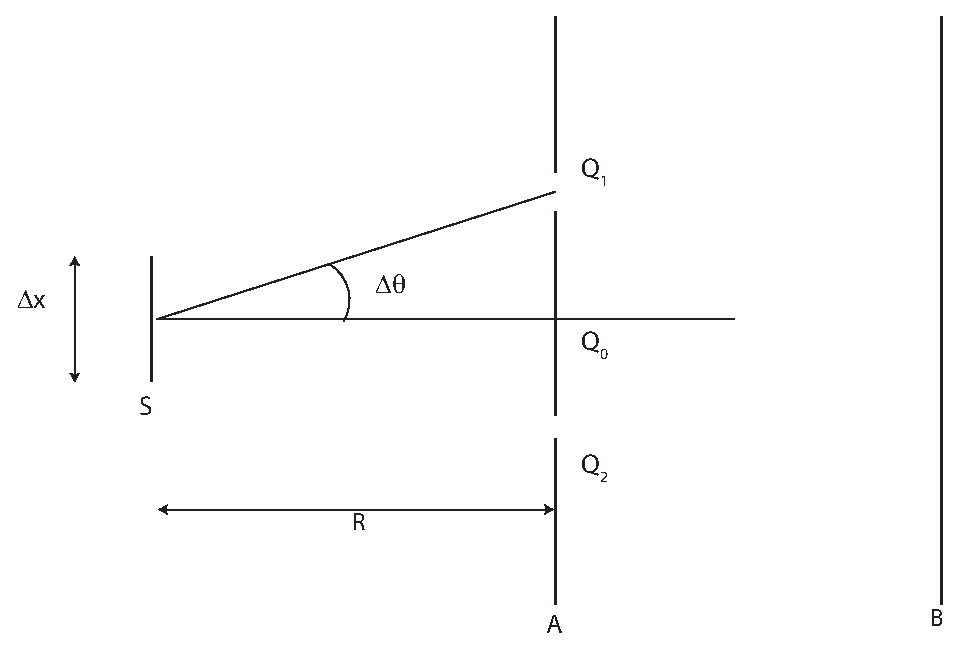
\includegraphics[width=.6\textwidth]{C:/Users/Massimo/Documents/Thesis/spatial_coherence.eps}
	\caption{\label{fig:spatialcoherence} Young experiment setup.}
\end{figure}
The area of coherence quantifies the degree of spatial coherence. It depends on the area of the light source S, the distance of observation R and the wavelength of the light. 
\subsection{Simulation of Spatial Coherence}
\label{sec:spatial}
A novel method for simulating spatial coherence that generates a source optical field with a degree of coherence defined by the user was developed and described below. An electromagnetic wave is generated by a dipole oscillating at a certain frequency. This dipole can be a molecule, an atom, a group of atoms in a gas. In case of a conventional incandescence light source light is emitted by tungsten atoms exited by the electrical current. This is also true for other sources of illuminations, like gas lamps, neon, or solid state light sources like LED; atoms of molecules excited to higher energy level emit light when dropping on the ground energy level. Each dipole emits light with a certain initial phase. Considering a light source of surface $\Sigma$ containing oscillating dipoles, the elemental surfaces $d\Sigma$ is defined as the surfaces on which all the dipoles oscillates with the same phase. The average dimension of the elemental surfaces $d\Sigma$ is proportional to the degree of spatial coherence of the light source. The more coherent the light source, the bigger the elemental surfaces will be. 
From a computational point of view having a light source composed of a mosaic of surfaces with different phases is equivalent to adding a phase mask to the input field. This phase mask is composed of areas with a random phase value. The dimension of these areas gives an idea of the degree of spatial coherence. The idea behind the empirical method used to generate the phase mask is shown in figure \ref{fig:phasemask1}: 
\begin{figure}[H]
	\begin{center}
		\begin{tabular}{c}
			\includegraphics[height=7cm]{C:/Users/Massimo/Documents/Thesis/coherence2.eps}
		\end{tabular}
	\end{center}
	\caption{ \label{fig:phasemask1} 
		A random phase mask is generated by propagating light coming form an array of sources, each one with a random phase value in the interval $[-\pi,\pi]$. }
\end{figure} 
An array of point sources is generated on a sampling window of the same dimension as the input field. The sources are placed regularly across the array. If the number of sources is less than $20 \times 20$, the sources are displaced randomly in order not to affect the coherence with their regular structure. The square of the number of point sources used is defined as the coherence index $C$. A \textit{C} of 100 means that the initial array is composed of 100 $\times$ 100 sources. A random phase value in the range $[-\pi,\pi]$ is assigned to each of these point sources. Their amplitude is set to one. Then the array of point sources is convolved with a kernel $K$ whose size is defined in order to make all the random point sources disks of amplitude one with a finite size. All this disks touch each others without overlapping as figure \ref{fig:phasemask2} shows. The size of the kernel depends on the resolution N of the input field and on the coherence index $C$ and is equal to the ratio $N/C$.\\
The result of the convolution is a phase mask that is formed by an array of circular areas with a random phase value.
Although this array of sources is already a phase mask, it cannot be used directly in the simulation platform because of its periodicity. In fact it is not a random phase pattern. In order to randomize the shape and the distribution of the coherence areas the array of sources is propagated at a distance bigger than the size of the sources. The distance $d_c$ chosen to propagate the light sources is the one derived in section \ref{sec:fresnelmulti} to keep the same sampling both in the input and output fields using the Fresnel propagation method discussed in section. From equation \ref{eq:getz3}:
\begin{equation}
\label{eq:propcoherence}
	d_c = \dfrac{W^2}{N\lambda}
\end{equation} 
where $W$ is the field of view, $N$ is the sampling and $\lambda$ is the wavelength of the light. The choice of using the Fresnel propagation as described in section \ref{sec:Fresnel} has been made because the propagation distance is small and hence aliasing issues do not arise. In addition to that it only requires one Fourier transform, making the random phase generation algorithm faster.
The whole process is shown in figure \ref{fig:phasemask2}
\newpage
\begin{figure}[H]
	\begin{center}
		\begin{tabular}{c}
			\includegraphics[height=15cm]{C:/Users/Massimo/Documents/Thesis/phasetarray200.eps}
		\end{tabular}
	\end{center}
	\caption	{ \label{fig:phasemask2} 
		Process of the creation of the phase mask. Top: array of point sources with a random phase value; centre: array of the areas of coherence at source after the convolution with $K$; bottom: randomized areas of coherence at object plane after the propagation of $d_c$. }
\end{figure} 
Some examples of phase masks generated from different number of sources can be seen in figure \ref{fig:phasemask3}:
\begin{figure}[H]
	\begin{center}
		\begin{tabular}{c}
			\includegraphics[height=15cm]{C:/Users/Massimo/Documents/Thesis/phi.eps}
		\end{tabular}
	\end{center}
	\caption{ \label{fig:phasemask3} 
		Final random phase mask generated a coherence index C equals to 10, 50, 100 and 200. }
\end{figure} 
The algorithm to generate the random phase mask can be summarized as follow:
\begin{itemize}
\item A number of light sources are defined, arranged in a regular array and allocated a random phase between $-\pi$ and $\pi$. 
 \item Each source has a size diameter given by: $N/C$
 \item This array of sources is then propagated a distance $d_c$ shown in equation \ref{eq:propcoherence} in order to randomize the shape of the coherence areas.
 \item the resultant phase is used as the output phase mask to add the input field.
\end{itemize}
\newpage
\subsection{Simulation of Temporal Coherence}
\label{sec:simtempcoherence}
 As discussed in section \ref{sec:temp}, temporal coherence is defined by the time $\tau$ in which the optical wave is correlated with itself. In other words after a time $t=\tau$, the optical disturbance $U(t)$ and $U(t+\tau)$ are totally uncorrelated and cannot interfere with each other. 
To simulate this effect many snapshots of the output field are taken each time using a different random distribution of phases for the sources. Assuming that the time difference between every snapshot is larger than or equal to the coherence time $\tau$. For the application for which this toolbox has been designed it is not relevant to know the exact value of $\tau$. However, the light source used for the laboratory prototype was a Thorlabs LED Array Light Source LIU630A with a wavelength centred on 630 nm and a bandwidth $\Delta\lambda=20 nm$. The emission spectrum is shown in figure \ref{fig:emission_spectrum}.
\begin{figure}[H]
	\begin{center}
		\begin{tabular}{c}
			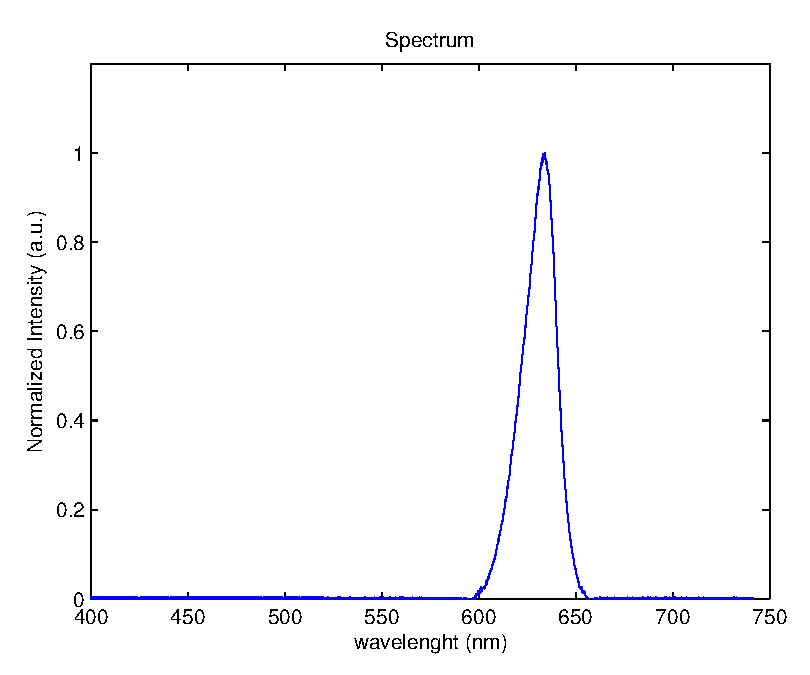
\includegraphics[height=7cm]{C:/Users/Massimo/Documents/Thesis/spectralLED.eps}
		\end{tabular}
	\end{center}
	\caption{ \label{fig:emission_spectrum} 
		Emission spectrum of the LED considered in our simulations and real image system. Data plotted from Thorlabs LED Array Light Source LIU630A datasheet. }
\end{figure} 
 Its coherence time is given by:
\begin{equation}
\label{key}
\tau = \dfrac{1}{\Delta\nu}=\dfrac{\Delta\lambda}{c}
\end{equation}
which is equal to $\tau=6.6\times10^{-17} s$. 
 Therefore each snapshot is assumed to be taken at the image plane at an interval of $\tau$. 
 All the snapshots are then added together, integrating the optical disturbance over time. Longer integration times will give better contrast and less noise while approaching to the incoherent imaging as it is shown in the following paragraph.
 \section{Optimization of Coherence Parameters}
 The previous section described how partially coherent light is simulated and how an algorithm that produces a certain number of snapshots of the output field, each one with a different random phase, was implemented. The random phase mask simulates the spatial coherence, the number of iteration instead simulates the effects of temporal coherence.
 \subsection{Optimization of Spatial Coherence}
 Simulations have been run propagating an optical disturbance with phase masks generated with different values of the parameter \textit{C}.
 The input field is the USAF resolution target, shown in figure \ref{fig:USAF}
 \begin{figure}[H]
 	\begin{center}
 		\begin{tabular}{c}
 			\includegraphics[height=4cm]{C:/Users/Massimo/Documents/Thesis/USAF.eps}
 		\end{tabular}
 	\end{center}
 	\caption{ \label{fig:USAF} 
 		USAF resolution target. }
 \end{figure} 
 The first simulation has been made changing the coherence index $C$ from a value of 5 (high coherence) to 500 (low coherence) in a sampling window with a resolution of 1765 by 1765 pixels.
 Figure \ref{fig:spatialsnr2} shows how the field at the image plane for different values of \textit{C} appears, while figure \ref{fig:spatialsnr1} shows a plot of the signal to noise ratio of the images as a function of the coherence index showing an asymptotic behaviour. After a certain threshold value of $C$, increasing the coherence index does not improve the image quality. The threshold is defined as the value of $C$ for which the variance of the previous five values of SNR is less then 0.01.
Figure \ref{fig:spatialsnr1} shows that for values of $C$ bigger than 250 the SNR asymptotically tends to 18 dB. In this case the resolution of the input field, and therefore of the phase mask, is 1765 by 1765 pixels, so that the SNR reaches the asymptote when the ratio between the number of sources and the resolution is 0.14. After this point, there is no gain in making the light source more incoherent in terms of signal to noise ratio improvement.
The ratio between the number of sources \textit{C} and the resolution of the optical field \textit{N} is defined as the incoherence degree $\iota$:
\begin{equation}
\label{eq:incoherence_degree}
\iota = \dfrac{C}{N}
\end{equation}
\begin{figure}[H]
 	\centering
 	\includegraphics[width=.5\textwidth]{C:/Users/Massimo/Documents/Thesis/iota.eps}
 	\caption{\label{fig:spatialsnr2}Images of the USAF resolution target with different values of $\iota$. Increasing the number of point sources generating the phase mask leads to more incoherent imaging, leading to improved resolution. Images where obtained with 300 iterations.}
 \end{figure}
 \begin{figure}[H]
 	\centering
 	\includegraphics[width=1\textwidth]{C:/Users/Massimo/Documents/Thesis/SNRspatial.eps}
 	\caption{\label{fig:spatialsnr1}Signal to noise ratio of the image of a USAF resolution target plotted as a function of the coherence index $C$.}
 \end{figure}
 \newpage
 \subsection{Optimization of Temporal Coherence}
The second simulation run aimed to define the optimum number of snapshots in order to correctly simulate temporal coherence. The random phase mask acts as a diffuser, and the resultant output field obtained by a single snapshot will present a low signal to noise ratio due to speckles, as shown in figure \ref{fig:speckle}
\begin{figure}[H]
	\centering
	\includegraphics[width=.5\textwidth]{C:/Users/Massimo/Documents/Thesis/USAF5iter.eps}
	\caption{\label{fig:speckle}Noise due to the speckles in an image of a USAF resolution target after only 5 iterations.}
\end{figure}
Taking several snapshots and adding them all together is equal to an integration over time of the optical field reaching the sensor. While increasing the integration time, the noise due to the speckles drops considerably. Figure \ref{fig:iter} shows several images of the USAF target in figure \ref{fig:USAF} taken with an incoherence degree of $\iota=0.14$, and with an increasing number of iterations form 5 to 1000.
 \begin{figure}[H]
 	\centering
 	\includegraphics[width=1\textwidth]{C:/Users/Massimo/Documents/Thesis/iter.eps}
 	\caption{\label{fig:iter}Images of the USAF resolution target obtained adding an increasing number of snapshot. this is equivalent to increase the integration time of the sensor. The noise due to the speckles caused by the phase mask decreases with increasing number of iterations.}
 \end{figure}
 Since increasing the number of iterations is computationally expensive, the signal to noise ratio of the images in figure \ref{fig:iter} has been evaluated and plotted as a function of the number of iteration in order to define an optimal parameter. Results are shown in figure \ref{fig:SNRiter}. The threshold is defined as the number of iterations for which the variance of the previous five values of SNR is less then 0.01.
 \begin{figure}[H]
 	\centering
 	\includegraphics[width=1\textwidth]{C:/Users/Massimo/Documents/Thesis/SNRtemporal.eps}
 	\caption{\label{fig:SNRiter}Signal to noise ratio as a function of the number of iterations. The threshold has been calculated looking at the variance of the previous five data.}
 \end{figure}
 For an image with an incoherence degree of $\iota=0.14$ the number of iterations after the SNR of the image does not improve further is 350. After that value the SNR tends asymptotically to 18 dB in spite of an increased computational effort. Therefore from a SNR point of view the optimal number of iteration to simulate temporal incoherence is 350. All the other simulations presented in this work will be performed with the coherence parameters discussed in this section. 
\subsection{Coherent Imaging vs Incoherent Imaging}
The image of an edge has been simulated to make a comparison between the coherent and the incoherent system response. Data were simulated with the same optical parameters described in section \ref{sec:system}. The intensity profile of an image of an edge is well known both in the case of coherent and incoherent illumination and provides a means of verification for the simulation methodology discussed above. Figure \ref{fig:coherenceprofile} shows the response of a coherent and an incoherent imaging systems to a sharp edge. The intensity profile of the edge is shown in green, its coherent image in blue and the incoherent image is shown in red. The coherent image presents fringes whose amplitude decreases further away form the edge. This effect is known as ringing artefacts, due to the coherent transfer function that usually presents rapid discontinuities \cite{goodman2005introduction}. Another property of the coherent image is that it crosses the actual location of the edge at 1/4 of its asymptotic value of intensity, while the incoherent image does the same at 1/2 of its asymptotic value, as can be seen in figure \ref{fig:coherenceprofile} \cite{goodman2005introduction}. Both conditions are verified by the simulations run as shown in figure \ref{fig:coherenceprofile}. \\
\\
\\
\begin{figure}[H]
	\centering
	\includegraphics[width=.9\textwidth]{C:/Users/Massimo/Documents/Thesis/2dedge.eps}
	\caption{\label{fig:coherenceprofile}Comparison between the coherent and an incoherent response of a simple 2f system to a sharp edge.}
\end{figure}
\nomenclature{$\overrightarrow{E}$}{Electric field}
\nomenclature{$\overrightarrow{H}$}{Magnetic field}
\nomenclature{$\epsilon$}{Electrical permittivity}
\nomenclature{$\mu$}{Magnetic permittivity}
\nomenclature{$\nabla$}{Laplacian operator}
\nomenclature{$\widehat{i},\widehat{j}$, $\widehat{k}$}{unit vectors}
\nomenclature{$n$}{Refractive index}
\nomenclature{$c$}{Speed of light in vacuum}
\nomenclature{$t$}{Time}
\nomenclature{$u$}{Field disturbance}
\nomenclature{$\nu$}{Optical frequency}
\nomenclature{$\phi$}{Phase}
\nomenclature{$k$}{Wave number}
\nomenclature{$U$}{Complex field}
\nomenclature{$\eta, \chi$}{Object space coordinates}
\nomenclature{$\sigma$}{Area of the aperture}
\nomenclature{$f_x, f_y$}{Spatial frequencies}
\nomenclature{$\nu_x, \nu_y$}{Local spatial frequencies}
\nomenclature{SNR}{Signal to noise ratio}
\nomenclature{$\Delta$}{Thickness function}
\nomenclature{$t_{lens}$}{Transmission of the lens}
\nomenclature{R}{Radius of curvature of a lens surface}
\nomenclature{$N$}{Number of samples}
\nomenclature{$r$}{Radius of a lens aperture}
\nomenclature{$F_\#$}{F-number}
\nomenclature{$\nu_c$}{Optical cut-off frequency}
\nomenclature{$x_{min}$}{Position of Airy Disk first minimum}
\nomenclature{$\Gamma$}{Autocorrelation function}
\nomenclature{$\tau$}{Coherence time}
\nomenclature{$A$}{Area}
\nomenclature{$\Delta S$}{Area of the emitting source}
\nomenclature{$d\Sigma$}{Elemental area}
\nomenclature{$C$}{Coherence index}
\nomenclature{$d_c$}{Distance of propagation in the coherence algorithm}
\nomenclature{$W$}{Size of the input optical field}
\nomenclature{$\iota$}{Incoherence degree}


\chapter{Fresnel Simulation Toolbox: applications}
\markboth{\MakeUppercase{Fresnel Simulation Toolbox: applications}}{}
\label{chap:fresnel2}
\section{Introduction}
This chapter will describes in details the performance of the different free space propagation operators described in the previous chapter. Some examples of how they can be used to simulate of an optical system will also be presented. Particular attention will be given to the differences between the different operators in terms of performance and signal to noise ratio.
It will also be largely described how to simulate partially coherent light. An original method to simulate both spatial and temporal coherence will be presented. Results form the numerical simulations will also be presented to support the theoretical model and to optimise the parameters.
In future developments of this work could be interesting to evaluate the performances of these methods analytically. But for the nature of this work is it enough to evaluate those performances using the simulations.
\section{Performances of the Angular Spectrum Methods}
 \label{sec:perfAS}
 To evaluate the differences in resolution of the three variants of the angular spectrum methods, normal Angular spectrum (AS), Band Limited Angular Spectrum (BL), and Corrected Band Limited Angular Spectrum (CBL) presented in chapter \ref{chap:fresnel}, a simulation has been implemented consisting of a free space propagation of a constant input field with a circular pupil of diameter 5 mm, sampled with a resolution of 3000 $\times$ 3000 pixels with a sampling window of 1 cm. The propagation distances \textit{z} varied from 1 m to 10 m. The wavelength used was of 633 nm, corresponding to the red Helium-Neon Laser. Performances have been evaluated experimentally through the simulations.\\ 
 The setup simulated is shown in figure \ref{fig:setup111}.
  \begin{figure}[h]
  	\begin{center}
  		\begin{tabular}{c}
  			\includegraphics[height=6cm]{perf1.eps}
  		\end{tabular}
  	\end{center}
  	 	\caption	{ \label{fig:setup111} 
  	 		Positions of the plane where the optical field has been sampled with respect to the aperture. }
  	 \end{figure} 
 Results are shown in figure \ref{fig:methods} where the cross section of the diffraction patterns are shown. 
 The BL method shown in the central column gives smooth diffraction patterns. Increasing the propagation distance however leads to the intensity profile losing part of the information because of the excessive low pass filtering on the propagation transfer function, leading the complete loss of the diffraction fringes. A comparison with the AS can be seen in figure \ref{fig:methods}, where the diffraction fringes are presents with the superimposition of the noise due to aliasing in the transfer function sampling. This affects the resolution of the diffraction pattern and the signal to noise ratio (SNR) drops with \textit{z} as shown in figure \ref{fig:SNR1}.The CBL method gives a good noise reduction without losing the original signal shape as explained in section \ref{sec:angular3} and as it is shown in figure \ref{fig:methods} on the far right column. Fringes are clearly present in the diffraction pattern even for large propagation distances and the noise is removed. \\
 In figure figure \ref{fig:SNR1} the SNR of the diffraction patterns in figure \ref{fig:methods} is plotted as a function of the propagation distance for the three examined cases. The BL method gives a better SNR especially for short propagation distances, where the bandwidth of the transfer function is not low pass filtering the signal yet, but only avoiding the aliasing. Its values remains in general above the SNR of the CBL method (almost 15dB), even in the case of large propagation distances. This is due to the excessive smoothing action that leads to the loss of resolution. On the other hand without any bandwidth limitation, AS, green line, the aliasing generated noise becomes dominant for long propagation distances and the SNR approaches the 0 dB value. The best results in terms of resolution and noise reduction are given by the corrected BL method where the information on the diffraction is retained entirely.
 \begin{figure}[H]
 	\begin{center}
 		\begin{tabular}{c}
 			\includegraphics[height=12cm]{SNR_com.eps}
 		\end{tabular}
 	\end{center}
 	\caption	{ \label{fig:SNR1} 
 		Sampling of the  Signal to Noise ratio (SNR) at various values of the propagation distances for the three propagation methods seen in section \ref{sec:angular 2}. The lines are just joining the sampled points and does not represent a model. The BL and the corrected BL methods improve the SNR, that instead drops as the propagation distance increases when the AS method is used. }
 \end{figure}
e 
 \begin{figure}[H]
 	\begin{center}
 		\begin{tabular}{c}
 			\includegraphics[height=15cm]{methods1.eps}
 		\end{tabular}
 	\end{center}
 	\caption{ \label{fig:methods} 
 		Comparison of the performances of the three angular spectrum propagation operator. Diffraction patterns of a 5mm pupil obtained by the simulations. On the left column are shown diffraction pattern cross section obtained using the angular spectrum method (AS). In the central column the pattern for the same propagation distances have been obtained using the band limited method (BL) and in the right column the same patterns have been obtained using the correct band limited method (corrected BL). }
 \end{figure}
 
 \section{Comparison between the Free Space Propagation Operators}
 \label{sec:comp}
	 In this section the differences in performance between the Fresnel approximation and the angular spectrum of plane waves approach will be shown with particular attention to the computational time required by the different methods, the optical resolution and the error. Results will be used to evaluate the characteristic of the different propagation operators. These results differ from the ones obtained in section \ref{sec:perfAS} since the simulations in this case involve the whole imaging system including the lens and not only the free space propagation.
	 \subsection{Description of the System}
	 \label{sec:system}
	 The system simulated is a simple imaging system composed of a single lens with focal length $f=158mm$, in a \textit{2f} configuration, as shown in figure \ref{fig:2f}. The field of view is a square of $1cm \times 1cm$, and the resolution of the input field is $2000 \times 2000$ pixels. The aperture of the lens is $D=5mm$ and its f number, defined as:
	 \begin{equation}
	 \label{eq:fnum}
		F_{\#}=\dfrac{z}{D}
	 \end{equation}
	 is equal to $F_{\#}=63$, where z is the distance from the lens to the image plane, that in a 2f configuration is equal to $z=2f=316mm$.
	 \begin{figure}[h]
	 	\begin{center}
	 		\begin{tabular}{c}
	 			\includegraphics[height=5cm]{C:/Users/Massimo/Documents/Thesis/Thesis_PhD/2f.eps}
	 		\end{tabular}
	 	\end{center}
	 	\caption{ \label{fig:2f} 
	 		Schematic of the 2f system simulated. f is the focal length, z the propagation distances, D is the aperture of the lens, w the field of view and N the sampling resolution. }
	 \end{figure} 
	 The optical cut-off frequency of this system is given by the relation \cite{goodman2005introduction}:
	 \begin{equation}
	 \label{eq:cutoff}
	 \nu_{co}=\dfrac{1}{\lambda F_{\#}}
	 \end{equation} 
	 The object was illuminated with monochromatic light of wavelength $\lambda=633nm$, therefore the cut-off frequency was $\nu_{co}=2.5\cdot10^4 cycles/m$.
	 \subsection{Image of a Point Source}
	 The first experiment simulated is the image of a point source, realized with a pinhole of $10 \mu m$ of diameter placed at the object plane indicated in figure \ref{fig:2f}. The image has been taken using four different methods to propagate the light into the system. Those are:
	 \begin{itemize}
	 	\item Multi step Fresnel method (MSF), section\ref{sec:fresnelmulti}
	 	\item Angular spectrum method (AS), section \ref{sec:angular}
	 	\item Band Limited Angular Spectrum method (BL), section \ref{sec:angular 2}
	 	\item corrected Band Limited Angular Spectrum method (CBL), section \ref{sec:angular3}
	 		 \end{itemize}
The impulse response for a point source as input will be computed using each of these methods.\\
 The sequence of operators used to simulate the system is shown in figure \ref{fig:sequence2} \\
	 \begin{figure}[H]
	 	\begin{center}
	 		\begin{tabular}{c}
	 			\includegraphics[height=1.8cm]{C:/Users/Massimo/Documents/Thesis/Thesis_PhD/imagesystem.eps}
	 		\end{tabular}
	 	\end{center}
	 	\caption{ \label{fig:sequence2} 
	 		Operator sequence for the 2f system. }
	 \end{figure} 
	 
	In the assumption of having a lens with a circular aperture and no aberrations, the impulse response of an optical system is an Airy Disk, that is the Fourier transform of the pupil of the system at the image plane. The fact that the theoretical output of the experiment is well known allows to determine the quality of the simulation tools.
	In addition to that, the Fourier transform of the impulse response of an optical system gives information on the frequencies content of the image, hence the band pass of the imaging system and its quality. 
	Figure \ref{fig:resultspoint11} shows the sensor image at the image plane together with intensity profiles of the image.
	\newpage
	 \begin{figure}[H]
	 	\begin{center}
	 		\begin{tabular}{c}
	 			\includegraphics[height=15cm]{C:/Users/Massimo/Documents/Thesis/Thesis_PhD/methodspoint1new.eps}
	 		\end{tabular}
	 	\end{center}
	 	\caption{ \label{fig:resultspoint11} 
	 		From top to Bottom: Image and intensity cross section of a point source according to multi step method, angular spectrum method, band limited angular spectrum method and corrected band limited angular spectrum method. In red is plotted the theoretical Airy pattern for reference. }
	 \end{figure} 
	From figure \ref{fig:resultspoint11} it can be seen that in the case of the MSF method the cross section of the impulse response does not go to zero because if additive background noise. In addition to that an offset is present in the image generated. This represent a reason more to discard the multi-step method form any future simulation. The response of the AS method has a high frequency noise components superimposed to the diffraction pattern while the BL method reduces the noise due to aliasing of the transfer function in the AS case as can be seen comparing the two cross sections. Both the BL and the CBL methods present no background noise and in the high frequency noise is reduced with respect to the AS case. Another parameter to evaluate the accuracy of these methods is the position of the Airy disk first minimum. It is given by \cite{goodman2005introduction,pedrotti1993introduction}:
	 \begin{equation}
	 \label{eq:airy}
	 x_{min}=1.22\dfrac{\lambda z}{D}
	 \end{equation}
	 where $D$ is the aperture of the lens. According to the values in section \ref{sec:system} the Airy disk should have a its first minimum at $x_{min}=67 \mu m$.
	 Without considering the MSF case that is too noisy and does not present zeros, the position of the first minimum is the other cases are:\\
	 \begin {table}
	 \begin{center}
	 	\label{tab:minimum}
	 \begin{tabular}{ l | r }
	 	
	 	\hline			
	 	AS & 67.5 $\mu m$ \\
	 	BL & 77.5 $\mu m$ \\
	 	CBL & 77.5 $\mu m$ \\
	 	\hline 
	 		\end{tabular}
	 			\caption{Position of the first minimum for all the three different angular spectrum methods. }
	\end{center}
\end{table}
	As expected for both the band limited angular spectrum methods (BL and CBL) the Airy Disk is slightly wider due to the low pass filtering action that transfer function has undergone.  However noise is reduced with the band limitation as shown in figure
	 \ref{fig:resultspoint11}.
	 The noise of each diffraction patter has been estimated considering as a reference the theoretical Airy patter. After subtracting it to the calculated intensity profile, the variance has been used to estimate the noise. Values of the variance for the three different angular spectrum methods are shown in table \ref{tab:noisemethods} :
	 	 \begin {table}
	 	 \begin{center}
	 	 	\label{tab:noisemethods}
	 	 	\begin{tabular}{ l | r }
	 	 		
	 	 		\hline	
	 	 		Method & variance \\
	 	 		\hline		
	 	 		AS & 0.00120000 \\
	 	 		BL & 0.00054646 \\
	 	 		CBL & 0.00056632 \\
	 	 		\hline 
	 	 	\end{tabular}
	 	 	\caption{Noise estimation for the three different angular spectrum methods. }
	 	 \end{center}
	 	\end{table}
	 To better understand how the resolution changes with the different methods, it is worth to have a look at the Fourier transform of the images shown in figure \ref{fig:resultspoint11}. The Fourier transform of the impulse response of a system give its frequency response. The shape of the frequency response gives information about how the frequency components of the input signal are modulated and transferred to the output signal. When this function goes to zero the correspondent frequency value is called the cutoff frequency. For frequencies higher than the cutoff frequency, all the information included in the input signal is lost. Results are shown in figure \ref{fig:resultspoint2}. The graphs are symmetric with respect to the zero frequency, therefore only the positive frequencies are shown.
	 
	 \begin{figure}[h]
	 	\begin{center}
	 		\begin{tabular}{c}
	 			\includegraphics[height=8cm]{C:/Users/Massimo/Documents/Thesis/Thesis_PhD/MTFnew.eps}
	 		\end{tabular}
	 	\end{center}
	 	\caption{ \label{fig:resultspoint2} 
	 		From top left to bottom right: Power spectrum of the image of a point source obtained with the MSF method, the AS method, the BL method and the CBL method. In red is plotted the theoretical Airy pattern power spectrum for reference. }
	 \end{figure} 
	From a comparison of the power spectra in figure \ref{fig:resultspoint2} it is possible to note the difference in shape of the power spectrum of the MSF method, that goes to zero slower than the angular spectrum methods spectra. These three figures present as expected the same shape since for low frequency the three angular spectrum methods are identical, with the difference of the frequency components after the cut-off frequency due to the fact that the BL and the CBL have narrower bandwidths. In the AS method graph a strong peak is present at a frequency of $10^5 m^{-1}$ due to digital artefacts arising from aliasing effects. This peak disappears in the other two band limited implementations of the angular spectrum. 
	It is interesting that all four power spectra present a dispersion of the energy towards high frequencies, indicating that a noise is not avoidable in the simulation toolbox.
\section{Coherence}
\label{sec:coherence}
The Fresnel simulation toolbox has been designed to analyse a light field imaging system. Since all current and most future applications of plenoptic systems will have incoherently illuminated objects, the simulation of such a systems should take it into account. Therefore the decision to develop an algorithm to simulate light propagating in a low state of coherence was taken. In addition to that low coherent illumination avoids interference pattern cross talk between neighbours lenslets that might decrease the quality of the final image. \\
Coherence is a statistical property of light and is described in terms of second order averages known as coherence functions \cite{goodman2015statistical,mandel1995optical}. A full analysis of coherence of optical fields can be found in text books such as Born and Wolf \cite{born1999principles}, Mandel and Wolf \cite{mandel1995optical} and Goodman \cite{goodman2015statistical} and will not be discussed in this work. For the application described in this work coherence will be treated under a less rigorous point of view. Before analysing the computational model of coherence it is worth examining the two different types of coherence. As defined by Goodman \cite{goodman2015statistical} :
\begin{itemize}
	\item \textbf{Temporal Coherence} can be defined as the ability of light to interfere with a delayed version of itself
	\item \textbf{Spatial Coherence} can be defined as the ability of light to interfere with a spatially shifted version of itself
\end{itemize}
The empirical method developed to simulate light propagating at low coherence includes both spatial and temporal coherence. 
\subsection{Temporal Coherence}
\label{sec:temp}
Following the explanation of Goodman \cite{goodman2015statistical}, given a complex disturbance $U(\overrightarrow{X},t)$ with a finite bandwidth $\Delta\nu $, it is expected to remain constant during a time interval $\tau<1/\Delta\nu$. This means that the disturbance taken at two different times in the same spatial position $U(\overrightarrow{X},t)$ and $U(\overrightarrow{X},t+\tau)$ are highly correlated if $\tau<\tau_c$ where $\tau_c$ is the coherence time. Under this condition $\tau_c=1/\Delta\nu$.
Since the correlation takes place without any spatial shift it is possible to drop the spatial coordinates $\overrightarrow{X}$. The degree of temporal coherence is therefore given by the autocorrelation function:
\begin{equation}
\label{eq:coherence1}
	\Gamma(\tau) =\langle U(t+\tau)U^*(t) \rangle
\end{equation}
The coherence time $\tau$ is therefore a function of the bandwidth of the light. A perfectly monochromatic plane wave has a very narrow bandwidth and a long coherence time, while on the other hand ultra fast laser pulses will have a short coherence time and a large bandwidth. From the coherence time it is possible to define the coherence length as $l_c= v\tau_c$ where $v=c/n$ is the speed of light in the medium of propagation given by the speed of light in the vacuum $c$ divided by the refractive index $n$.
\subsection{Spatial Coherence}
To analyse spatial coherence two complex disturbances $U(\overrightarrow{X}_1,t)$ and $U(\overrightarrow{X}_2,t)$ are observed at the same time in two different position $\overrightarrow{X}_1$ and $\overrightarrow{X}_2$. When the two points coincide, $\overrightarrow{X}_1=\overrightarrow{X}_2$ the two disturbances are perfectly correlated. When the distance between the two points begins to increase, the correlation degree decreases until they become totally uncorrelated. In order to better understand this concept it is useful to illustrate the Young experiment \cite{wolf2007introduction}. With reference to figure \ref{fig:spatialcoherence} a squared light source of size $\Delta x$ emits light towards a screen at a distance R. On the screen A there are two pinholes $Q_1$ and $Q_2$. In order to have interference fringes on a second screen B the following condition should be satisfied:
\begin{equation}
\label{eq:fringes}
\Delta x \Delta \theta < \lambda
\end{equation} 
Where $2\Delta\theta$ is the angle formed at the source with the two pinholes $Q_1$ and $Q_2$ and $\lambda$ is the wavelength of the light emitted by the source. In order to see the fringes, the two pinholes should be situated in an area $\Delta A$ of size:
\begin{equation}
\label{eq:area1}
\Delta A \sim (R \Delta \theta)^2 = \dfrac{R^2}{S}\lambda
\end{equation} 
R is the distance between the screen A and the source, $S=\Delta x^2$ is the area of the source, and equation \ref{eq:fringes} has been used. The area $\Delta A$ is the coherence area of the light in the plane $A$ around the point $Q_0$ on the optical axis. 
 \begin{figure}[H]
	\centering
	\includegraphics[width=.6\textwidth]{C:/Users/Massimo/Documents/Thesis/Thesis_PhD/spatial_coherence.eps}
	\caption{\label{fig:spatialcoherence} Young experiment setup.}
\end{figure}
The area of coherence quantifies the degree of spatial coherence. It depends on the area of the light source S, the distance of observation R and the wavelength of the light. 
\subsection{Simulation of Spatial Coherence}
\label{sec:spatial}
The goal of this section is to define a novel method for simulating spatial coherence in order to generate partially coherent optical fields. An electromagnetic wave is generated by a dipole oscillating at a certain frequency. This dipole can be a molecule, an atom, a group of atoms in a gas. In case of a conventional incandescence light source, light is emitted by tungsten atoms excited by the electrical current. This is also true for other sources of illuminations, like gas lamps, neon, or solid state light sources like LED; atoms of molecules excited to higher energy levels emit light when dropping to the ground energy level. Each dipole emits light with a certain initial phase. Considering a light source of surface $\Sigma$ containing oscillating dipoles, the elemental surfaces $d\Sigma$ is defined as the surfaces on which all the dipoles oscillate with the same phase. The average size and dimensionality of the elemental surfaces $d\Sigma$ is proportional to the degree of spatial coherence of the light source. The more coherent the light source, the bigger the elemental surfaces will be. 
From a computational point of view having a light source composed of a mosaic of surfaces with different phases is equivalent to adding a phase mask to the input field. This phase mask is composed of areas with a random phase value. The dimension of these areas gives an idea of the degree of spatial coherence. The idea behind the empirical method used to generate the phase mask is shown in figure \ref{fig:phasemask1}: 
\begin{figure}[H]
	\begin{center}
		\begin{tabular}{c}
			\includegraphics[height=7cm]{C:/Users/Massimo/Documents/Thesis/Thesis_PhD/coherence2.eps}
		\end{tabular}
	\end{center}
	\caption{ \label{fig:phasemask1} 
		A random phase mask is generated by propagating light coming form an array of sources, each one with a random phase value in the interval $[-\pi,\pi]$. }
\end{figure} 
An array of point sources is generated on a sampling window of the same dimension as the input field. The sources are placed regularly across the array. If the number of sources is less than $20 \times 20$, the sources are displaced randomly in order not to affect the coherence with their regular structure. The square root of the number of point sources used is defined as the coherence index $C$. A \textit{C} of 100 means that the initial array is composed of 100 $\times$ 100 sources. A random phase value in the range $[-\pi,\pi]$ is assigned to each of these point sources. Their amplitude is set to one. Then the array of point sources is convolved with a kernel $K$ whose size is defined in order to make all the random point sources disks of amplitude one with a finite size. All these disks touch each others without overlapping as figure \ref{fig:phasemask2} shows. The size of the kernel depends on the resolution N of the input field and on the coherence index $C$ and is equal to the ratio $N/C$.\\
The result of the convolution is a phase mask that is formed by an array of circular areas with a random phase value.
Although this array of sources is already a phase mask, it cannot be used directly in the simulation platform because of its periodicity. In fact it is not a random phase pattern. In order to randomize the shape and the distribution of the coherence areas the array of sources is propagated at a distance bigger than the size of the sources. The distance $d_c$ chosen to propagate the light sources is the one derived in section \ref{sec:fresnelmulti} to keep the same sampling both in the input and output fields using the Fresnel propagation method discussed in section. From equation \ref{eq:getz3}:
\begin{equation}
\label{eq:propcoherence}
	d_c = \dfrac{W^2}{N\lambda}
\end{equation} 
where $W$ is the field of view, $N$ is the sampling and $\lambda$ is the wavelength of the light. The choice of using the Fresnel propagation as described in section \ref{sec:Fresnel} has been made because the propagation distance is small and hence aliasing issues do not arise. In addition to that it only requires one Fourier transform, making the random phase generation algorithm faster.
The whole process is shown in figure \ref{fig:phasemask2}
\newpage
\begin{figure}[H]
	\begin{center}
		\begin{tabular}{c}
			\includegraphics[height=15cm]{C:/Users/Massimo/Documents/Thesis/Thesis_PhD/phasetarray200.eps}
		\end{tabular}
	\end{center}
	\caption	{ \label{fig:phasemask2} 
		Process of the creation of the phase mask. Top: array of point sources with a random phase value; centre: array of the areas of coherence at source after the convolution with $K$; bottom: randomized areas of coherence at object plane after the propagation of $d_c$. }
\end{figure} 
Some examples of phase masks generated from different number of sources can be seen in figure \ref{fig:phasemask3}:
\begin{figure}[H]
	\begin{center}
		\begin{tabular}{c}
			\includegraphics[height=15cm]{C:/Users/Massimo/Documents/Thesis/Thesis_PhD/phi.eps}
		\end{tabular}
	\end{center}
	\caption{ \label{fig:phasemask3} 
		Final random phase mask generated a coherence index C equals to 10, 50, 100 and 200. }
\end{figure} 
The algorithm to generate the random phase mask can be summarized as follow:
\begin{itemize}
\item A number of light sources are defined, arranged in a regular array and allocated a random phase between $-\pi$ and $\pi$. 
 \item Each source has a size diameter given by: $N/C$
 \item This array of sources is then propagated a distance $d_c$ shown in equation \ref{eq:propcoherence} in order to randomize the shape of the coherence areas.
 \item the resultant phase is used as the output phase mask to add the input field.
\end{itemize}
These considerations lead to correct results as proven by the simulation of the image of an edge presented in section \ref{sec:coherencevsinco}.
\newpage
\subsection{Simulation of Temporal Coherence}
\label{sec:simtempcoherence}
 As discussed in section \ref{sec:temp}, temporal coherence is defined by the time $\tau$ in which the optical wave is correlated with itself. In other words after a time $t=\tau$, the optical disturbance $U(t)$ and $U(t+\tau)$ are totally uncorrelated and cannot interfere with each other. 
To simulate this effect many snapshots of the output field are taken each time using a different random distribution of phases for the sources. Assuming that the time difference between every snapshot is larger than or equal to the coherence time $\tau$. For the application for which this toolbox has been designed it is not relevant to know the exact value of $\tau$. However, the light source used for the laboratory prototype, that will be described in chapter \ref{chap:microscope}, was a Thorlabs LED Array Light Source LIU630A with a wavelength centred on 630 nm and a bandwidth $\Delta\lambda=20 nm$. The emission spectrum is shown in figure \ref{fig:emission_spectrum}.
\begin{figure}[H]
	\begin{center}
		\begin{tabular}{c}
			\includegraphics[height=7cm]{C:/Users/Massimo/Documents/Thesis/Thesis_PhD/spectralLED.eps}
		\end{tabular}
	\end{center}
	\caption{ \label{fig:emission_spectrum} 
		Emission spectrum of the LED considered in our simulations and real image system. Data plotted from Thorlabs LED Array Light Source LIU630A datasheet. }
\end{figure} 
 Its coherence time is given by:
\begin{equation}
\label{key}
\tau = \dfrac{1}{\Delta\nu}=\dfrac{\Delta\lambda}{c}
\end{equation}
which is equal to $\tau=6.6\times10^{-17} s$. 
 Therefore each snapshot is assumed to be taken at the image plane at an interval of $\tau$. 
 All the snapshots are then added together, integrating the optical disturbance over time. Longer integration times will give better contrast and less noise while approaching to the incoherent imaging as it is shown in the following paragraph.
 \section{Optimization of Coherence Parameters}
 In this section simulation will be presented in order to estimate the best values of the simulation parameters to produce partially coherent light. These parameters are the coherence coefficient $C$ for spatial coherence and the number of snapshots for the temporal coherence. A resolution target was imaged by a 2f system described in section \ref{sec:system}.
 \subsection{Optimization of Spatial Coherence}
 Simulations have been run propagating an optical disturbance with phase masks generated with different values of the parameter \textit{C} with the purpose of defining the optimal number of sources to generate a phase mask that produces a final images with a high signal to noise ratio.
 The input field used is the USAF resolution target, shown in figure \ref{fig:USAF}
 \begin{figure}[H]
 	\begin{center}
 		\begin{tabular}{c}
 			\includegraphics[height=3cm]{C:/Users/Massimo/Documents/Thesis/Thesis_PhD/USAF.eps}
 		\end{tabular}
 	\end{center}
 	\caption{ \label{fig:USAF} 
 		USAF resolution target. }
 \end{figure} 
 The first simulation has been made changing the coherence index $C$ from a value of 5 (high coherence) to 500 (low coherence) in a sampling window with a resolution of 1765 by 1765 pixels.
 Figure \ref{fig:spatialsnr2} shows how the field at the image plane for different values of \textit{C} appears, while figure \ref{fig:spatialsnr1} shows a plot of the signal to noise ratio of the images as a function of the coherence index showing an asymptotic behaviour. After a certain threshold value of $C$, increasing the coherence index does not improve the image quality. The threshold is defined as the value of $C$ for which the variance of the previous five values of SNR is less than 0.01.
 Figure \ref{fig:spatialsnr1} shows that for values of $C$ bigger than 250 the SNR asymptotically tends to 18 dB. In this case the resolution of the input field, and therefore of the phase mask, is 1765 by 1765 pixels, so that the SNR reaches the asymptote when the ratio between the number of sources and the resolution is 0.14. After this point, there is no gain in making the light source more incoherent in terms of signal to noise ratio improvement.
 \begin{figure}[H]
 	\centering
 	\includegraphics[width=.4\textwidth]{C:/Users/Massimo/Documents/Thesis/Thesis_PhD/iota.eps}
 	\caption{\label{fig:spatialsnr2}Images of the USAF resolution target with different values of $\iota$. Increasing the number of point sources generating the phase mask leads to more incoherent imaging, leading to improved resolution. Images where obtained with 300 iterations.}
 \end{figure}
 The ratio between the number of sources \textit{C} and the resolution of the optical field \textit{N} is defined as the incoherence degree $\iota$:
 \begin{equation}
 \label{eq:incoherence_degree}
 \iota = \dfrac{C}{N}
 \end{equation}
 \newpage
 
 \begin{figure}[H]
 	\centering
 	\includegraphics[width=1\textwidth]{C:/Users/Massimo/Documents/Thesis/Thesis_PhD/SNRspatial.eps}
 	\caption{\label{fig:spatialsnr1}Signal to noise ratio of the image of a USAF resolution target plotted as a function of the coherence index $C$.}
 \end{figure}
 The image quality evaluated using the signal to noise ratio improves with the increasing of the sources used to generate the phase mask. However it reaches an asymptote after 250 sources. This is due to the fact that the interference effects due to low coherence decrease, improving image quality. 
 \newpage
 \subsection{Optimization of Temporal Coherence}
The second simulation run aimed to define the investigate the effect of increasing the number of snapshots on temporal coherence effects. The random phase mask acts as a diffuser, and the resultant output field obtained by a single snapshot will present a low signal to noise ratio due to speckles, as shown in figure \ref{fig:speckle}
\begin{figure}[H]
	\centering
	\includegraphics[width=.5\textwidth]{C:/Users/Massimo/Documents/Thesis/Thesis_PhD/USAF5iter.eps}
	\caption{\label{fig:speckle}Noise due to the speckles in an image of a USAF resolution target after only 5 snapshots.}
\end{figure}
Taking several snapshots and adding them all together is equal to an integration over time of the optical field reaching the sensor. While increasing the integration time, the noise due to the speckles drops considerably. Figure \ref{fig:iter} shows several images of the USAF target in figure \ref{fig:USAF} taken with an incoherence degree of $\iota=0.14$, and with an increasing number of snapshots from 5 to 1000.
 \begin{figure}[H]
 	\centering
 	\includegraphics[width=1\textwidth]{C:/Users/Massimo/Documents/Thesis/Thesis_PhD/iter.eps}
 	\caption{\label{fig:iter}Images of the USAF resolution target obtained adding an increasing number of snapshot. this is equivalent to increase the integration time of the sensor. The noise due to the speckles caused by the phase mask decreases with increasing number of snapshots. images are obtained summing the snapshots, therefore they do not have the same brightness.}
 \end{figure}
 Since increasing the number of snapshots is computationally expensive, the signal to noise ratio of the images in figure \ref{fig:iter} has been evaluated and plotted as a function of the number of snapshots in order to define an optimal parameter. Results are shown in figure \ref{fig:SNRiter}. The threshold is defined as the number of snapshots for which the variance of the previous five values of SNR is less then 0.01.
 \begin{figure}[H]
 	\centering
 	\includegraphics[width=1\textwidth]{C:/Users/Massimo/Documents/Thesis/Thesis_PhD/SNRtemporal.eps}
 	\caption{\label{fig:SNRiter}Signal to noise ratio as a function of the number of iterations. The threshold has been calculated looking at the variance of the previous five data. The purpose of the fitted curve is to show the asymptotic behaviour of the data.}
 \end{figure}
 For an image with an incoherence degree of $\iota=0.14$ the number of iterations after which the SNR of the image does not improve further is 350. After that value the SNR tends asymptotically to 18 dB in spite of an increased computational effort. Therefore from a SNR point of view the optimal number of iteration to simulate temporal incoherence is 350. All the other simulations presented in this work will be performed with the coherence parameters discussed in this section. 
\subsection{Coherent Imaging vs Incoherent Imaging}
\label{sec:coherencevsinco}
The image of an edge has been simulated to make a comparison between the coherent and the incoherent system response. Data were simulated with the same optical parameters described in section \ref{sec:system}. The intensity profile of an image of an edge is well known both in the case of coherent and incoherent illumination and provides a means of verification for the simulation methodology discussed above. Figure \ref{fig:coherenceprofile} shows the response of a coherent and an incoherent imaging systems to a sharp edge. The intensity profile of the edge is shown in green, its coherent image in blue and the incoherent image is shown in red. The coherent image presents fringes whose amplitude decreases further away from the edge. This effect is known as ringing artefacts, due to the coherent transfer function that usually presents rapid discontinuities \cite{goodman2005introduction}. Another property of the coherent image is that it crosses the actual location of the edge at 1/4 of its asymptotic value of intensity, while the incoherent image does the same at 1/2 of its asymptotic value, as can be seen in figure \ref{fig:coherenceprofile} \cite{goodman2005introduction}. Both conditions are verified by the simulations run as shown in figure \ref{fig:coherenceprofile}. \\
\\
\\
\begin{figure}[H]
	\centering
	\includegraphics[width=.9\textwidth]{C:/Users/Massimo/Documents/Thesis/Thesis_PhD/2dedge.eps}
	\caption{\label{fig:coherenceprofile}Comparison between the coherent and an incoherent response of a simple 2f system to a sharp edge.}
\end{figure}
\section{Conclusions}
In this  chapter it was shown how the methods described in chapter \ref{chap:fresnel} can be implemented by the simulation toolbox. A comparison between the different free space propagation methods described in chapter \ref{chap:fresnel} was presented in section \ref{sec:perfAS} showing how the corrected band limited angular spectrum method is the most suitable to simulate an imaging system since presents the best trade-off between computational performance, Signal to Noise ration and accuracy of the output field. This has been proven further in section \ref{sec:comp} where the image of a point source obtained with the four different method has been analysed both in the spatial and frequency domain. \\
The last two sections of this chapter discuss coherence and present an original method to simulate partially coherent light sources. The method is described in details and an estimation of the best simulation parameters is presented. The correctness of the results is proven through the simulation of an infinite edge presented in section \ref{sec:coherencevsinco}. 
\nomenclature{$\overrightarrow{E}$}{Electric field}
\nomenclature{$\overrightarrow{H}$}{Magnetic field}
\nomenclature{$\epsilon$}{Electrical permittivity}
\nomenclature{$\mu$}{Magnetic permittivity}
\nomenclature{$\nabla$}{Laplacian operator}
\nomenclature{$\widehat{i},\widehat{j}$, $\widehat{k}$}{unit vectors}
\nomenclature{$n$}{Refractive index}
\nomenclature{$c$}{Speed of light in vacuum}
\nomenclature{$t$}{Time}
\nomenclature{$u$}{Field disturbance}
\nomenclature{$\nu$}{Optical frequency}
\nomenclature{$\phi$}{Phase}
\nomenclature{$k$}{Wave number}
\nomenclature{$U$}{Complex field}
\nomenclature{$\eta, \chi$}{Object space coordinates}
\nomenclature{$\sigma$}{Area of the aperture}
\nomenclature{$f_x, f_y$}{Spatial frequencies}
\nomenclature{$\nu_x, \nu_y$}{Local spatial frequencies}
\nomenclature{SNR}{Signal to noise ratio}
\nomenclature{$\Delta$}{Thickness function}
\nomenclature{$t_{lens}$}{Transmission of the lens}
\nomenclature{R}{Radius of curvature of a lens surface}
\nomenclature{$N$}{Number of samples}
\nomenclature{$r$}{Radius of a lens aperture}
\nomenclature{$F_\#$}{F-number}
\nomenclature{$\nu_c$}{Optical cut-off frequency}
\nomenclature{$x_{min}$}{Position of Airy Disk first minimum}
\nomenclature{$\Gamma$}{Autocorrelation function}
\nomenclature{$\tau$}{Coherence time}
\nomenclature{$A$}{Area}
\nomenclature{$\Delta S$}{Area of the emitting source}
\nomenclature{$d\Sigma$}{Elemental area}
\nomenclature{$C$}{Coherence index}
\nomenclature{$d_c$}{Distance of propagation in the coherence algorithm}
\nomenclature{$W$}{Size of the input optical field}
\nomenclature{$\iota$}{Incoherence degree}


\chapter{Simulations of a Plenoptic 1.0 System}
\markboth{\MakeUppercase{Simulations of a Plenoptic 1.0 System}}{}
\label{chap:chapter4}
\section{Introduction}
\label{sec:intro3}
The main purpose of the work described in this chapter is to prove that the images obtained simulating a plenoptic imaging system using the wave simulation toolbox described in chapter \ref{chap:fresnel} are equivalent to the ones obtained with conventional ray tracing techniques. In addition to that the effects of diffraction will be explained and evaluated. Simulations were run also to better understand the existing rendering algorithms, the synthetic refocusing algorithm and depth estimation. These algorithms based on ray optics give the expected results on the raw images produced using the wave optics simulation toolbox.
The methods used to design, develop and test the data processing algorithms, such as rendering, synthetic refocus and depth estimation algorithms from the digitally generated light fields data are described. All the light field processing algorithms presented in this chapter use the third parametrization of the light field described in section \ref{sec:LFparam} that is the four dimensional representation of the intensity recorded on the sensor. Each point of this four dimensional array is a ray at the position \textit{x} and \textit{y} with a direction $\theta_x$ and $\theta_y$ \cite{ng2006digital,georgiev2010focused}.
\section{Description of the System}
\label{sec:system10}
The plenoptic 1.0 camera described in section \ref{sec:camera10} has been modelled as a 2f system composed of a main lens, a micro lens array and a sensor as shown in figure \ref{fig:pleno10_system}. The micro lens array is placed at a distance \textit{z=2f} from the main lens, where \textit{f} is the focal length of the main lens, and the sensor is placed at a distance $f_\mu$ from the micro array plane that is also the focal length of the lenslets. In this configuration the lenslet array plane is conjugated with the object plane, while the sensor plane is conjugated with the main lens plane. In order to satisfy the f-number matching condition described in section \ref{sec:camera10} the software automatically sets the aperture of the main lens according to the propagation distances, the micro lens array parameters, the resolution \textit{N} of the input field, the wavelength of the light used and the micro array parameters settings. 
\begin{figure}[H]
	\centering
	\includegraphics[width=.7\textwidth]{C:/Users/Massimo/Documents/Thesis/Thesis_PhD/plenoptic101.eps}
	\caption{\label{fig:pleno10_system} Parameters that characterize the micro lens array are: the pitch $p$, defined as the distance between the centres of two lenslets, the diameter d, the number of lenslets per row N and the size of the micro array W. }
\end{figure}
The micro array parameters are illustrated in figure \ref{fig:microarray1} and are the pitch, the diameter of the single lenslet, the number of lenslet in a row and the size of the array. In all simulations the pitch of the lenslets is equal to the diameter and the lenslets are arranged in a square matrix. 
\begin{figure}[H]
	\centering
	\includegraphics[width=.7\textwidth]{C:/Users/Massimo/Documents/Thesis/Thesis_PhD/micro_array.eps}
	\caption{\label{fig:microarray1} Parameters that characterize the micro lens array. }
\end{figure}
\subsection{Diffraction Effects on the System}
\label{sec:diffraction}
Diffraction from the lenslet's circular aperture can generate cross talk between neighbouring sub images since the light form a single lenslet falls in the sub image of the neighbouring lenslet. Because of this, blur is present in the rendered image resulting in a loss of spatial resolution. To avoid this loss of resolution the diameter of each lenslet should be large enough so that the diameter of the Airy disk is smaller than the lenslet diameter. As seen in equation \ref{eq:airy} for a lens with a circular aperture, the diameter of the Airy disk at its focal plane is
\begin{equation}
\label{eq:airy1}
d_{Airy} = 2.44\lambda z/d
\end{equation}
 In order to avoid diffraction induced cross talk the lenslet diameter should be:
\begin{equation}
\label{eq:lenscond}
D>2.44 \dfrac{\lambda z}{D}
\end{equation} 
Therefore the condition of \textit{D} is:
\begin{equation}
\label{eq:min_diam}
D>\sqrt{2.44\lambda f_{\mu}}
\end{equation}
This is a very important result and it is an original contribution to the field, since it represents the first design condition ever evaluated form diffraction considerations. 
Therefore when choosing or designing a lenslet array for plenoptic imaging the lenslet diameter and the focal length should satisfy equation \ref{eq:min_diam}. The acceptable values belong to the area above the blue line in the diagram shown in figure \ref{fig:mindiam}.
\begin{figure}[H]
	\centering
	\includegraphics[width=.7\textwidth]{C:/Users/Massimo/Documents/Thesis/Thesis_PhD/mindiameter.eps}
	\caption{\label{fig:mindiam} Values of acceptable lenslet diameter to avoid diffraction induced cross talk. }
\end{figure}
The effect of cross talk between lenslets on the raw image is shown in figure \ref{fig:crosstalk1}.
This image was obtained simulating a point source imaged by a 120 mm lens placed in a 2f configuration with the lens let array. The sensor resolution was 2000 by 2000 pixels and the micro array was made of 101 by 101 lenslets with a diameter of 100 $\mu$m and a focal length of 100 mm.
\begin{figure}[H]
	\centering
	\includegraphics[width=.4\textwidth]{C:/Users/Massimo/Documents/Thesis/Thesis_PhD/crosstalk1.eps}
	\caption{\label{fig:crosstalk1} Raw plenoptic image of a point source. The grid represents the edges of the sub images. If the point source is in focus, it should be represented by only one lenslet. Because of diffraction some light goes also on the neighbouring sub images. }
\end{figure}
\begin{figure}[H]
	\centering
	\includegraphics[width=1\textwidth]{C:/Users/Massimo/Documents/Thesis/Thesis_PhD/phasespacefocused2.eps}
	\caption{\label{fig:crosstalk2}Phase space of the light field of a point object: on the left is the case when the condition \ref{eq:min_diam} is respected; on the right when diffraction induces cross talk that arises between neighbouring lenslets. Cross talk introduces a blur in the rendered image whose width is $\Delta x$. }
\end{figure}
Figure \ref{fig:crosstalk2} shows what happens in the phase space of a point source in the presence of cross talk and without cross talk. In the first case there is no blur since all the light coming from a point source in focus is recorded by a single lenslet, while in the second case the spreading of the light due to diffraction causes a blur that is proportional to the number of sub images involved. 
\section{Advanced Rendering Techniques}
As described in chapter \ref{chap:chapter1}, one pixel in the rendered image is obtained from the mean of all the pixels of the sub image that corresponds to the position of the pixel in the final image \cite{ng2006digital}. This method generates an image that is equivalent to the image obtained with a conventional camera without any additional information. Since the final resolution depends on the number of lenslets in the micro array, it will be smaller than the resolution that can be obtained by a conventional camera which instead uses the full sensor resolution \cite{georgiev2010focused}. To use the full variety of features enabled by light field imaging, more advanced post processing techniques of the raw data should be used. The first two post processing features presented are the change of aperture and of point of view. These effects are achieved by integrating each sub image along a sub set of directional coordinates, hence on a smaller number of pixels. 
\subsection{Changing Aperture}
The quality of the image captured by a conventional camera depends on the combination of shutter speed and aperture chosen in order to get the optimum total exposure \cite{pedrotti1993introduction}.
 The possibility of changing the aperture of the main lens in post processing allows us to change the depth of field of the final image. In the simulations presented in this work the shutter speed is not an issue since all the objects imaged static with constant and uniform illumination. Therefore what determines the exposure is the aperture of the main lens or the f-number. The f-number is proportional to the depth of field of the imaging system that can be defined as the range of depths that appears sharp in the resulting photograph \cite{ng2006digital}. If the f-number increases and the aperture gets smaller, the depth of field increases. Therefore a plenoptic camera can control the depth of field in post processing.
 Looking at the raw plenoptic image, each sub image is formed by a number of samples of the directions of the rays. If in equation \ref{eq:rendering2} the range of integration along the directional coordinates is reduced, the aperture of the main lens is reduced at the same amount. If the aperture is smaller the rays propagating with a large angle with respect to the optical axis will not reach the sensor and will be not considered to form the intensity of each pixel. The result is a rendered image that looks like it has been captured with a narrower aperture. Computationally the algorithm to reduce the aperture is:
 \begin{equation}
 	\label{eq:rendering4}
 	I(x,y) = \dfrac{1}{N'^2}\sum_{i=k_x/2}^{N-\frac{k_x}{2}}\sum_{j=k_{y}/2}^{N-\frac{k_y}{2}} L(x,y,i,j)
 \end{equation}
 where $N'=N-k$ and \textit{k} is the range of directional coordinates considered in the sum. This operation in the phase space is shown in figure \ref{fig:rendering4}:
 \begin{figure}[H]
 	\centering
 	\includegraphics[width=.7\textwidth]{C:/Users/Massimo/Documents/Thesis/Thesis_PhD/renderingape.eps}
 	\caption{\label{fig:rendering4} Rendering seen from the $(x,\theta_x)$ slice of the phase space. The directional pixels not considered for the integration are shown in grey. }
 \end{figure}
An effect of reducing the aperture of a camera is to extend its depth of field. Therefore the depth of field can be digitally extended changing the range of directional coordinates included in the sum as explained above.
Figure \ref{fig:rawstanford1} shows the raw image of thin silky skin separating two layers of an onion, immersed in oil to improve transparency. The image is obtained from the online repository of raw plenoptic data provided by Levoy in Syanford University \cite{levoy2006microscope}. 
 Figure shows \ref{fig:stanford1} the differences between the rendered image integrating over the full aperture, and the rendered image obtained using only the central pixel of each sub image. The effect is to reduce the aperture to a pinhole and to have an all-in-focus image.
 Images has been obtained with home made rendering algorithm written in MATLAB.
 \begin{figure}[H]
 	\centering
 	\includegraphics[width=.4\textwidth]{C:/Users/Massimo/Documents/Thesis/Thesis_PhD/rawst.eps}
 	\caption{\label{fig:rawstanford1} Raw plenoptic 1.0 image obatined from Levoy \textit{et al.} The microscope was a Zeiss Axiovert with a 20x/0.5NA (dry) objective. The micro lens array was 24mm x 36mm, with square 125-micron x 125-micron f/20 micro lenses, held in front of the Axiovert's side camera port using an optical bench mount. The camera was a Canon 5D full-frame digital SLR. The specimen was the thin silky skin separating two layers of an onion, immersed in oil to improve transparency \cite{levoy2006microscope}. }
 \end{figure}
\begin{figure}[H]
	\centering
	\includegraphics[width=0.9\textwidth]{C:/Users/Massimo/Documents/Thesis/Thesis_PhD/stanfordfull.eps}
	\caption{\label{fig:stanford1}Rendered Images from the raw data in figure \ref{fig:rawstanford1}. On the left there is the full aperture image obtained integrating along all the directional coordinates, while on the right there is the all in focus image obtained taking only the central pixel of the each sub image, that corresponds to rays with the direction parallel to the optical axis.}
\end{figure}
 \subsection{Changing the Point of View}
It is possible to change the point of view in the rendered image integrating along all the directional coordinates in one direction keeping fixed the other direction. For example an image corresponding to a particular point of view can be obtained, with reference to equations \ref{eq:rendering5}, keeping fixed the directional coordinate corresponding to the desired point of view and integrating along all the other coordinates. 
 \begin{equation}
 \label{eq:rendering5}
 \begin{matrix}
 I(x,y)=\dfrac{1}{N}\sum_{i=0}^{N} L(x,y,i,k_y) \\
 \\
 I(x,y)=\dfrac{1}{N}\sum_{j=0}^{N} L(x,y,k_x,j)
 \end{matrix} 
 \end{equation}
 \section{Depth Estimation}
 \label{sec:depth10}
 This section discuss how depth information can be extracted from light field data. In the specific case of plenoptic 1.0 raw data, depth can be decoded looking at the phase space. Section \ref{sec:phase_space} explained that a point source on the focal plane of the main lens looks like a straight vertical line in the phase space. The physical meaning of this is that for a single position, that is one lenslet, all the directional coordinates are sampled \cite{georgiev2010focused}. If the point source is out of focus the situation is different. If the source is closer to the main lens with respect to the focal plane, it will be imaged on a plane that is behind the micro array. This situation is shown in figure \ref{fig:depth}. Both directional and positional coordinates are sampled by more than one lenslet and each sub image will sample a set of directional coordinates corresponding to the part of the main lens from where the rays come. Figure \ref{fig:depth1} shows what happens in the phase space. On the lenslet plane the spot size will have a width of $\Delta x$ proportional to the distance, therefore the directions will be sampled by the lenslets included in this interval. Each lenslet receives light coming  a particular area of the main lens, its correspondent sub image only records the pixels linked with those coordinates as can be seen comparing figure \ref{fig:depth} with \ref{fig:depth1}. The resultant phase space representation is still a straight line, but with positive slope proportional to the distance of the point source \ref{fig:depth1}. If the source is further away from the plane where the main lens is focused, the main lens image is formed before the lenslets plane. The point is still sampled by more than one lenslet included in the spot size $\Delta x$. The difference with the previous case is that now in the phase space the point source is represented by a straight line with a negative slope. The physical meaning of the slope of the phase space line can be understood by looking at figure \ref{fig:depth3}. When the main lens image is formed in front of the micro lens plane the increasing values of $\theta_x$ axis are mapped on decreasing values of x and the line on the phase space representing the point has a negative slope. If the image is formed behind the micro lens plane increasing directions on $\theta_x$ axis are mapped on increasing positions on the x axis this inversion is absent and the line in the phase space has a positive slope \cite{ng2006digital}. This characteristic of the phase space permits us to discriminate between points in the scene that are in front or behind the main lens focal plane, giving a first rough depth estimate. 
 \begin{figure}[H]
 	\centering
 	\includegraphics[width=.9\textwidth]{C:/Users/Massimo/Documents/Thesis/Thesis_PhD/defocous10.eps}
 	\caption{\label{fig:depth} Sampling of the light field of a point source in focus, on the top, closer to the main lens, centre, and further away, bottom. When the source is out of focus, both position and directions are sampled by more than one lenslet since the main lens image is no longer formed any more on the lenslet plane. }
 \end{figure}
 \begin{figure}[H]
 	\centering
 	\includegraphics[width=.6\textwidth]{C:/Users/Massimo/Documents/Thesis/Thesis_PhD/phasespacerefocus10.eps}
 	\caption{\label{fig:depth1} Information on the depth of a point source imaged by a plenoptic 1.0 system. As explained in section \ref{sec:phase_space}. If the point source is in focus, on the top, its position is sampled by one lenslet as well as the whole set of directions.}
 \end{figure}
 \begin{figure}[H]
 	\centering
 	\includegraphics[width=.7\textwidth]{C:/Users/Massimo/Documents/Thesis/Thesis_PhD/slope.eps}
 	\caption{\label{fig:depth3} Physical meaning of the slope in the phase space. If the point source is further then the camera focal plane, the phase space line has a negative slope. If the point source is closer then the focal plane, the slope of the phase space line is positive.}
 \end{figure}
 Plenoptic 1.0 camera simulations, as discussed above, have been run to verify this fact. The system was composed of a main lens with a focal length of \textit{120 mm}, in a \textit{2f} configuration creating an image on the micro array plane. The Micro lens array was composed of a matrix of 101 $\times$ 101 lenslets with a diameter of 100 $\mu m$ and a focal length of 100 \textit{mm}. The ensor had a resolution of 200 by 2000 pixels.
 \begin{figure}[H]
 	\centering
 	\includegraphics[width=.7\textwidth]{C:/Users/Massimo/Documents/Thesis/Thesis_PhD/defocus10.eps}
 	\caption{\label{fig:depth4} Numerical simulation of a point source imaged by a plenoptic 1.0 imaging system. The point source was placed at three different distances from the main lens. The top three figures show the focused image. In the centre ones a defocus of 0.125 m closer to the main lens is added. In the bottom ones the point source is closer to the main lens of 0.25 m. In all the three cases the raw data image is on the left, the rendered image is on the centre and the phase space line is on the right.}
 \end{figure}
 \newpage
 \section{Synthetic Refocus}
 \label{sec:refocus10}
Another post processing feature enabled by collecting the light field is the possibility to refocus an image after it has been captured. This features is called synthetic refocusing and is based on the fact that the recorded light field can be used to compute images as if they were taken by a synthetic camera positioned and focused differently from the actual camera. In this section the synthetic refocusing algorithm is explained in terms of the discussion in Ng \cite{ng2006digital} and Ng \textit{et al.} \cite{ng2005light}. \\
This method is based on the fact that for a plane out of focus for the real camera, it is possible to define a synthetic camera composed of an aperture and a sensor plane that is focused on that particular plane. The image produced by the synthetic camera will result in focus. This method is based on a synthetic camera model obtained with ray tracing. It can be implemented in a wave optics approach using the simulation platform developed in this work and the limitations and the issues arising from a wave approach with respect to the simple and ideal ray optics approach will be discussed. 
 Figure  \ref{fig:synthetic0} shows a plenoptic 1.0 imaging system whose main lens produces an out of focus image on the micro lens plane. The directional set of coordinates $\Delta u$ is mapped along the range of spatial coordinates $\Delta x$. The light field can be reparametrized in terms of a synthetic light field generated by an aperture on the plane \textit{u'} represented by the dashed lens, that focuses the object on a synthetic focal plane, \textit{x'}. This second light field is parametrized with the coordinates \textit{u' v'} and \textit{x' y'}. 
 \newpage
 \begin{figure}[H]
 	\centering
 	\includegraphics[width=.8\textwidth]{C:/Users/Massimo/Documents/Thesis/Thesis_PhD/sinth0.eps}
 	\caption{\label{fig:synthetic0} The synthetic camera refocusing method is based on the fact that is always possible to define a virtual aperture that is focused on the lenslet plane. }
 \end{figure}
 As explained by Ng \textit{et al.} \cite{ng2005light} and in analogy with what was explained in section \ref{sec:rendering1} it is possible to define the intensity obtained rendering a synthetic light field $L'(x',y', u', v') $ at the synthetic focal plane as:
 \begin{equation}
 \label{eq:sinth1}
 I(x,y)=\iint L'(x',y',u',v')A(u',v') du'dv'
 \end{equation}
 The goal is to express this intensity as a function of the captured light field $L(x,y,u,v)$ present on the actual sensor plane, finding the relationship that links the set of coordinates \textit{x, y, u, v} with \textit{x', y', u', v'}. 
 \newpage
 \subsection{Synthetic Refocus Algorithm}
 This algorithm has been developed by Ng \textit{et al.} \cite{ng2005light}. To find the link between the real and the synthetic light field the following simplifications are made: 
 \begin{itemize}
 	\item only the synthetic sensor plane \textit{x', y'} will be moved. Therefore the main lens plane \textit{u', v'} is at the same position of the plane \textit{u, v}, and no transformation is performed on the directional coordinates, therefore (\textit{u, v})=(\textit{u', v'}).
 	\item the aperture of the main lens will not change, $A(x', y')=1$.
 \end{itemize} 
 Figure \ref{fig:synthetic3} shows a two dimensional diagram explaining the reparametrization under the simplifications explained above. Only the coordinates x and u are shown for simplicity. F is defined as the distance of the main lens from the lenslet array plane, and F' as the distance from the synthetic focal plane. The ratio between these two distances is the refocusing parameter $ \alpha'$, defined as: 
 \begin{equation}
 	\label{eq:alpha}
 	 \alpha' = \dfrac{F}{F'}
 \end{equation}
 The refocusing factor can assume the following values:
 \begin{itemize}
 	\item $ \alpha'=1$ when the synthetic focal plane is at the same position of the main lens focal plane
 	\item $ \alpha'>1$ when the distance between the main lens and the synthetic 
 	image plane is smaller than the distance between the main lens and its original focal plane. This occurs when the system is refocused on a plane that it is further away with respect to the main lens focal plane.
 	\item $ \alpha'<1$ when the distance between the main lens and the synthetic image plane is bigger than the distance between the main lens and its original focal plane. This occurs when the refocus takes place on a plane that is closer with respect to the main lens.
 \end{itemize}
 \begin{figure}[H]
 	\centering
 	\includegraphics[width=.8\textwidth]{C:/Users/Massimo/Documents/Thesis/Thesis_PhD/refocus2.eps}
 	\caption{\label{fig:synthetic3} Changing the focal plane of the camera is equal to reparametrizing the light field according to the new coordinates. The reparametrization corresponds to a scaling of the ratio between the refocused plane and the original camera plane $ \alpha'$. }
 \end{figure}
 Looking at figure \ref{fig:synthetic3} a ray of light that crosses the main lens plane at the coordinate $u$ and that then intercepts the synthetic image plane at the point $x'_1$, can be represented with the coordinates of the original image plane $x_1$. Because of similar triangles, the value of the \textit{x} coordinate on the image plane can be expressed as a function of the coordinates $ u, x'$:
 \begin{equation}
 	\label{eq:refocus11}
 	x_1 = u+(x'_1-u)\dfrac{F}{F'}=u+(x'_1-u) \alpha'
 \end{equation}
 Therefore extending to the four dimensional case, the points belonging to the synthetic image plane can be expressed as a function of the directional coordinates at the main lens plane and the spatial coordinates at the original image plane as:
 \begin{equation}
 \label{eq:shear1}
 \begin{matrix}
 x' = \dfrac{x}{ \alpha'}+u\left(1-\dfrac{1}{ \alpha'}\right) \\
 \\
 y' = \dfrac{y}{ \alpha'}+v\left(1-\dfrac{1}{ \alpha'}\right)
 \end{matrix} 
 \end{equation}
 With this change of coordinates the light field at the synthetic focal plane $x'$ can be written substituting equations \ref{eq:shear1} into equation \ref{eq:sinth1}.
 \begin{equation}
 \label{eq:synthLF2}
 I(x,y) =\iint L\left(\dfrac{x}{ \alpha'}+u\left(1-\dfrac{1}{ \alpha'}\right),\dfrac{y}{ \alpha'}+v\left(1-\dfrac{1}{ \alpha'}\right),u,v\right)A(x',y')dudv
 \end{equation}
 Equation \ref{eq:synthLF2} represents the rendered image obtained by integrating along the directional coordinates of the light field reparametrized as if it were captured by a camera whose focal plane is the same as the synthetic focal plane. \\
 Focusing at different depths corresponds to changing the separation between the lens and the image plane, shifting it by a quantity proportional to the refocusing factor $ \alpha'$. From equation \ref{eq:shear1} the four dimensional light field at the synthetic plane is obtained from the light field recorded on the sensor by shifting and rescaling its spatial coordinates. The transformation operated on the light field is the composition of two transformations:
 \begin{itemize}
 	\item a scaling of a factor $ \alpha'$ that depends on the distance of the synthetic focal plane from the main lens.
 	\item a translation term $u(1-1/ \alpha')$ that increases with the directional coordinates and with the magnitude of the factor $ \alpha'$.
 	 \end{itemize} 
 	 Therefore the synthetic refocus can be treated as a linear operator acting on the four dimensional light field that maps the light field recorded on a new set of coordinates. The rendering on this new set of coordinates gives the image focused at a different plane.
\subsection{Refocusing Operator}
The synthetic refocus equation \ref{eq:synthLF2} has been obtained with ray optics considerations only. However, it can be applied to light fields obtained with wave optics simulations. When using wave optics particular attention should be given in the design of the imaging system in order to avoid cross talk effects induced by diffraction, as explained in section \ref{sec:diffraction}. The effects of this operator in the phase space is a change of the slope of the lines describing the points of the image in the phase space. Since the total light field is conserved, the area in the phase space remains the same, hence the projection of the light field on the phase space is sheared with respect to the original one \cite{georgiev2010focused}.
\begin{figure}[H]
	\centering
	\includegraphics[width=.8\textwidth]{C:/Users/Massimo/Documents/Thesis/Thesis_PhD/shear1.eps}
	\caption{\label{fig:shear1} Changing the position of the focal plane is equal to shear the light field in the phase space. The total area remains the same since the total light field is conserved. }
\end{figure}
 MATLAB code has been developed to implement the synthetic refocus operator. The algorithm is composed of two distinct stages. The first stage creates a new set of spatial coordinates shifting and rescaling the original set of coordinates as shown in equation \ref{eq:shear1}. Then the output synthetic light field is created interpolating the input light field using as a base the new set of coordinates. The flow chart can be seen in figure \ref{fig:flowcharet1}

\begin{figure}[H]
	\centering
	\includegraphics[width=.8\textwidth]{C:/Users/Massimo/Documents/Thesis/Thesis_PhD/flowshear.eps}
	\caption{\label{fig:flowcharet1} Flow chart of the operator shearing. }
\end{figure} 
\section{Results of the Simulations}
To test and explore the potentials of the synthetic refocusing algorithm the wave optics simulation toolbox described in section \ref{chap:fresnel} has been used. The System simulated is the one described in section \ref{sec:system} and shown in figure \ref{fig:pleno10_system2}. The optical parameters can be found in the following table. These parameters have been chosen in order to minimize the phase aliasing in the lens, to avoid diffraction induced cross-talk between the lenslets and to match the f-number of the main lens with the lenslets.
\\
\\
\begin{table}
	\centering
\begin{tabular}{l|r}

	Main lens focal length f & 120 mm\\ \hline
	Lens aperture D & 3.6 mm \\ \hline
	Micro lens focal length $f_{\mu}$ & 10 mm \\ \hline
	Micro lens diameter d & 150 $\mu m$ \\ \hline
	Micro array pitch p & 150 $\mu m$ \\ \hline
	Sensor size & 20 mm \\ \hline
	f-number & 33.6\\ \hline
	sensor resolution & 3030 by 3030 pixel \\ \hline	
%   
\end{tabular}
\caption{\label{tab:1} Simulations parameters. }
\end{table}

\begin{figure}[H]
	\centering
	\includegraphics[width=.7\textwidth]{C:/Users/Massimo/Documents/Thesis/Thesis_PhD/plenoptic101.eps}
	\caption{\label{fig:pleno10_system2} Set up of a plenoptic 1.0 camera replicated in the simulations. }
\end{figure}		
With this set up the final rendered image resolution iss 101 $\times$ 101 pixel. Each pixel of the final image corresponds to a lenslet, therefore the spatial resolution the final image is equal to the diameter of a single lenslet. Each sub image has 30 $\times$ 30 pixels, meaning that the full set of directional coordinates is sampled by $N_{sub}=30$ samples. The angular resolution is therefore:
\begin{equation}
\label{eq:angularres}
\delta\theta = \dfrac{\Delta\theta}{N_{sub}}=\dfrac{NA}{N_{sub}}
\end{equation}
and is equal to $\delta\theta = 2.5 10^{-4} rad$.\\
The first object to be imaged was a volume V of dimension 20 mm $\times$ 20 mm $\times$ 100 mm containing three point sources. Each point source has been simulated by a circle of 10 $\mu m$ diameter and are positioned as shown in figure \ref{fig:volumepoint}
\begin{figure}[H]
	\centering
	\includegraphics[width=.7\textwidth]{C:/Users/Massimo/Documents/Thesis/Thesis_PhD/planes.eps}
	\caption{\label{fig:volumepoint} Position of the point sources imaged inside the volume V simulated. }
\end{figure}
Each plane has been imaged independently setting the distance $z_1$ equal to the sum of the distance of the main lens focal plane and the defocus $\delta z$. The Coordinates of the points are: 
\begin{itemize}
	\item A: $x_1 = -3 mm , \quad y_1 = -3 mm , \quad z_1 = -50 mm$
	\item B: $x_2 = 0 mm, \quad y_2 = 0 mm, \quad z_2 = 0 mm$ 
	\item C: $x_3 = +3 mm , \quad y_3 = +3 mm, \quad z_3 = +50 mm$
	\end{itemize} 
Following the simulated propagation of the three planes through the system, the final output raw image has been obtained by summing the three separate raw images normalized by the total amount of energy contained. This can be done since the Fresnel simulation toolbox is time independent. Figure \ref{fig:rawandimage} shows the total raw image and the rendered image integrated without any refocusing.
\begin{figure}[H]
	\centering
	\includegraphics[width=.7\textwidth]{C:/Users/Massimo/Documents/Thesis/Thesis_PhD/refocus1.eps}
	\caption{\label{fig:rawandimage} Raw image on the left and rendered image on the right. Intensity is shown in false colour in order to appreciate variations in energy distribution. }
\end{figure}
The central spot is in focus, since the point source is at a distance of \textit{z = 2f} on the main lens focal plane.
For a defocus of 50 mm the factor $ \alpha'$ can be obtained from the lens equation. For the 2f system simulated and referring to figure \ref{fig:synthetic3} for notations:
\begin{equation}
\label{eq:alpha1}
\dfrac{1}{f} =\dfrac{1}{F'}+\dfrac{1}{(z+\Delta z)} 	
\end{equation}
Since $ \alpha' = F/F'$, and in a 2f system F=2f=z:
\begin{equation}
\label{eq:alpha2}
\dfrac{1}{f} =\dfrac{ \alpha'}{2f}+\dfrac{1}{(2f+\Delta z)} 	
\end{equation}
Resolving for $ \alpha'$ becomes:
\begin{equation}
\label{eq:alpha3}
 \alpha' = \dfrac{2f+s\Delta z}{2f+\Delta z} 	
\end{equation}
Figure \ref{fig:alpha} shows the values of $ \alpha'$ obtained by equation \ref{eq:alpha3} for defocus varying between plus and minus 10 cm.
\begin{figure}[H]
	\centering
	\includegraphics[width=.7\textwidth]{C:/Users/Massimo/Documents/Thesis/Thesis_PhD/alphadef.eps}
	\caption{\label{fig:alpha} Values of the refocusing factor $ \alpha'$ as a function of the defocus. A positive defocus means that the object it further away with respect to the main lens, a negative defocus indicates an object that is closer. }
\end{figure}
Figure \ref{fig:alpha} shows that, as expected, the refocus factor is not linear with defocus and therefore the axial resolution in not linear. When the object is closer to themain lens, small variations in the defocus give large variations in $ \alpha'$ while the opposite happens when the object is further away with respect to the main lens. \\
Figure \ref{fig:refocus} shows the refocused imaged obtained from shearing the light field extracted by the raw image in figure \ref{fig:rawandimage} on the left. According to equation \ref{eq:alpha3}, the point A is refocused for a value of $ \alpha'$ equal to 0.7 and point B for $ \alpha' = 1.17$.
\begin{figure}[H]
	\centering
	\includegraphics[width=.7\textwidth]{C:/Users/Massimo/Documents/Thesis/Thesis_PhD/refocus3point.eps}
	\caption{\label{fig:refocus} Refocused images of the three point sources in figure \ref{fig:rawandimage}. In the top one the point A is refocused, in the bottom one the point B is refocused. When the point source is refocused, the intensity distribution is higher with respect to the out of focus points. }
\end{figure}
The effects of the refocusing operator can be appreciated by looking the intensity values of the refocused point sources. In the top image of figure \ref{fig:refocus} the point labelled with the letter A is refocused, and the majority of the light present in the image concentrates on its location. The same happens in bottom figure, where the brightest point, indicated in red according to the colour bar, is the refocused one (B). This is a proof of the fact that the refocusing operator, shearing the four dimensional light field, moves the intensity from a location to another. The total energy of the image remains unchanged. 
\\
\section{Focal Stack Depth Estimation} 
The synthetic refocus algorithm provides a method to estimate the depth of a point source in a volume. This is an original contribution to the field and it is a proof of concept that depth information can be evaluated from the blur of the image. It has been treated only for the case of imaging a point source for simplicity. Further work should be done to extend it to larger more complex objects. Looking at the Fourier transform of a rendered image of a point source before and after the refocusing operation shows that when the point source is in focus, its spectrum is broader than the blurred one. This fact is true for general images as well, when the presence of sharp details in the focused image, causes its spectrum to have a larger amount of high spatial frequencies, and therefore more energy at high frequencies. Figure \ref{fig:spec1} is shows the difference between the spectrum of the out of focus image (blue) and the in focus image (red) for a defocus of 5 cm.
\begin{figure}[H]
	\centering
	\includegraphics[width=1\textwidth]{C:/Users/Massimo/Documents/Thesis/Thesis_PhD/spectrum2.eps}
	\caption{\label{fig:spec1} Spectrum of out of focus image (blue) and spectrum of the refocused image (red). }
\end{figure}
The action of shearing the light field produces a redistribution of the power spectrum of the signal towards high frequencies. \\
 This effect can be used to estimate the depth of the object imaged by evaluating its level of blur. This blur based depth estimation is an original contribution of this work to light field literature. The method consists in creating a focal stack by shearing the light field at different values of the coefficient $ \alpha'$, that correspond to different focal planes, and rendering the images. After the focal stack is created the power spectrum of each image is calculated using the fast Fourier transform algorithm. The low frequency terms are then removed by high pass filtering the images and the total energy contained in the high frequency term is calculated by integrating the Fourier spectra. The bandwidth of the high pass filter has been calculated in order to remove the central lobe of the spectrum. Plotting the values of energy as a function of the different $ \alpha'$ coefficients a curve with a maximum in the proximity of the most in focus image is obtained. This maximum corresponds to the image in the focal stack that best estimates the actual value of $ \alpha'$. Figure \ref{fig:maxima} shows the energy as a function of the refocus parameter $ \alpha'$ for a point source placed at different depths. The vertical red line indicates the position of the maximum. The values of the estimated $ \alpha'$ and the real one are shown in the following table:
 \\
 \\
 \begin{table}
  \begin{tabular}{l|c|c|r}
  	\hline
  	Estimated $ \alpha'$ & Real $ \alpha'$ & Error & Defocus \\ \hline
  	0.85 & 0.738 & 0.1132 & -0.05 m\\ \hline
  	0.925 & 0.8837 & 0.0413 & -0.025 m\\ \hline 
  	1.080 & 1.0943 & -0.0143 & +0.025 m\\ \hline
  	1.105 & 1.1724 & 0.0674 & +0.05 m\\ \hline
  	\label{tab:2}
  \end{tabular}
  \caption{Comparison between the estimated and the real values of the refocusing factor $ \alpha$ }
 \end{table}

Figure \ref{fig:error} shows the distribution of the estimated values of $ \alpha'$ versus the actual values obtained from equation \ref{eq:alpha3}.
 The estimated values for a defocus of -0.1 m and - 0.08 m are equal to 1 as if the image would lie on the focal plane. These are clearly wrong estimations and represent a limitation for the method described. It is interesting to see that for negative defocus the parameter $ \alpha'$ is over estimated and the error is positive while for positive defocus the error is negative. The minimum error is present for values of defocus corresponding to positions close to the focal plane. The error in the estimation of the refocusing factor is plotted in figure \ref{fig:error1}.
 \\
 Having seen these results the method has a better accuracy in a range of depth around the focal plane and performs worse when the absolute value of the defocus increases.
 These results show that the depth evaluation depends on the distance of the object from the camera. This is a natural consequence of the non linearity of the lens equation. A way to have a linear dependency of the parameter $ \alpha'$ with the refocusing distance is to have an array of lenslet with variable focal length \cite{wetzstein2011computational,georgiev2012multifocus}, or changing the focal length of the lenslets dynamically using electro optics effects \cite{ueda2008multi}.
 \begin{figure}[H]
 	\centering
 	\includegraphics[width=1\textwidth]{C:/Users/Massimo/Documents/Thesis/Thesis_PhD/depthsp.eps}
 	\caption{\label{fig:maxima} Energy contained in the spectrum of the rendered image plotted as a function of the refocusing factor $ \alpha'$. In red is indicated the value of $ \alpha'$ corresponding to the image with the maximum energy. }
 \end{figure}
\begin{figure}[H]
	\centering
	\includegraphics[width=.7\textwidth]{C:/Users/Massimo/Documents/Thesis/Thesis_PhD/errors1.eps}
	\caption{\label{fig:error} Estimated values of $ \alpha'$ represented by blue stars and the theoretical values represented with the red line. }
\end{figure}
\begin{figure}[H]
	\centering
	\includegraphics[width=.7\textwidth]{C:/Users/Massimo/Documents/Thesis/Thesis_PhD/errors2.eps}
	\caption{\label{fig:error1} Distance between the estimated values of $ \alpha'$ and the actual theoretical values. }
\end{figure}
The great difference between the theoretical and the estimated values of $\alpha'$ for defocus smaller than -0.02 m indicates that the method is not reliable when the object is too close to the main lens. Therefore those values should be discarded.
\section{Conclusions}
This chapter showed the results obtained simulating a plenoptic 1.0 imaging system using the Fresnel simulation toolbox described in chapter \ref{chap:fresnel}. With these simulation has been possible to evaluate for the first time the effects of diffarctions on the final image. An important result of this chapter is that the post processing algorithms obtained from ray optics theoretical models can be used to process raw images generated with a wave optics approach. This wave optics approach also led to the evaluation of the effects of diffraction on a plenoptic 1.0 system. A lenslet can be considered as a circular aperture whose diffraction pattern os the well known airy disk. If the fringes of the diffraction pattern of a lenslet extend on the neighbouring lenslet, cross-talk arise. To avoid the minimum diameter of a lenslet as indicated in equation \ref{eq:min_diam}.\\
The next step was to apply the rendering algorithm based on ray optics considerations already presented in literature and apply them on the raw images obtained from the wave optics simulations. All these methods gave the expected results proving that the simulation toolbox is capable to procuce realistic data. Particular attention was given to the depth estimation algorithm. With the help of the simulations it was possible to better understand and verify how the depth of an object can be estimated looking at the phase space. For a point source in focus the phase space look like a vertical straight line. if the point source is closer to the main lens the phase space will have a negative slope, while if it is further away from the main lens it will have a positive slope. This results perfectly match the theory. The synthetic refocus algorithm was also extensively analysed. Although this is not an original contribution to the field, it has been used to develop an original depth estimation method based on the creation of a focal stack of a point source refocused at different depth. It consist in refocusing the image of a point source at different depths and evaluate its power spectrum. The depth of the focal plane whose spectrum has the minimum energy will be value that better approximate the actual depth of the point source.\\
In coclusion, this chapter represents a link between the ray optics theoretical analysis of plenoptic imaging system extensively present in literature and its extension to wave optics. 
\nomenclature{$d_{Airy}$}{Airy disk diameter}
\nomenclature{$A'$}{Synthetic aperture}
\nomenclature{$ \alpha'$}{Refocusing factor}
\nomenclature{$F$}{Main lens - micro array distance}
\nomenclature{$F'$}{Main lens - synthetic focal plane distance}
\nomenclature{p}{Micro array pitch}
\nomenclature{$\delta\theta$}{Angular resolution}
\nomenclature{$N_{sub}$}{Sub-image resolution}

\chapter{Simulation of a Plenoptic 2.0 System}
\markboth{\MakeUppercase{Simulations of a Plenoptic 2.0 System}}{}
\label{chap:chapter5}
This chapter describes the simulations done to characterize the optical performances of a focused plenoptic imaging system. The scope of this work is to investigate the behaviour of a plenoptic 2.0 imaging system at its diffraction limit under a wave optics approach.  All simulations described in this chapter have been run using the Fresnel Simulation Toolbox  described in chapter \ref{chap:fresnel}. In a plenoptic 1.0 imaging system the resolution is limited by the dimensions of the lenslets \cite{georgiev2009resolution} and the final rendered image has a much lower resolution then a conventional image. In a focused plenoptic system, as explained in section \ref{sec:phase2.0}, the resolution of the final rendered image is not linked any more to the number of lenslet in the micro array and it is possible to recover the full sensor resolution pushing it even to sub-pixel resolution \cite{lumsdaine2008full,lumsdaine2009focused,georgiev2009superresolution}. This characteristic makes plenoptic systems suitable to a wider range of applications where high spatial resolution is required \cite{wetzstein2011computational}. In the past years further effort has been made to push plenoptic 2.0 system to achieve super-resolution performances \cite{georgiev2012super,georgiev2009superresolution,bishop2009light}. Here the term super-resolution is not referred to the achievement of a resolution beyond diffraction limit\cite{georgiev2015plenoptic} but to a digital sub pixel resolution only. When applied to microscopy diffraction still represents a big limitation for plenoptic imaging systems. This chapter will discuss how diffraction affects the optical resolution of an imaging system and how it is linked to the spatio-angular trade off \cite{georgiev2006spatio}. Numerical simulations will be implemented using by the platform described in chapter \ref{chap:fresnel}. 
\label{sec:intro4}
\section{Rendering in Plenoptic 2.0}
\label{sec:rendering}
As introduced in chapter \ref{chap:chapter1}, rendering an image form plenoptic 2.0  raw data is based on integrating for each position all the correspondent directional coordinates. While in plenoptic 1.0 each position is sampled by a single lenslet, which causes the loss of resolution in the final image, in plenoptic 2.0 each position is sampled by several lenslets. Therefore with reference to figure \ref{fig:render202}, the spatial coordinate (x,y) of point $A$ will be sampled by the lenslets 1, 2 and 3, therefore $A$ is represented by 3 sub images. Each sub image is a different point of view of A and directional coordinates are sampled by these three points of view simultaneously. The number of sub images into which the point \textit{A} is imaged depends on the magnification \textit{m=b/a} of the lenslet array and is given by:
\begin{equation}
\label{eq:point_of_view}
N_{sub} = \dfrac{1}{m}=\dfrac{a}{b}
\end{equation}
 \textit{a} is the distance of the micro array from the main lens image and \textit{b} is the distance of the from the sensor plane. 
\begin{figure}[H]
	\centering
	\includegraphics[width=.8\textwidth]{C:/Users/Massimo/Documents/Thesis/rendering201a.eps}
	\caption{\label{fig:render202} Top: the point $A$ is imaged by the main lens into the point $A'$. It is imaged by the lenslet array into a number of sub images depending by the magnification of the micro array stage, in this case \textit{m=0.333}. Bottom: particular of the raw image of the point source $A$ and phase space diagram. The three sub images \textit{1, 2} and \textit{3} are three different points of view of the object.  }
\end{figure}
From a computational point of view the basic rendering is performed directly on the raw sensor image and has the following steps:
\begin{itemize}
	\item the single sub images are isolated from each other 
	\item depending on the magnification \textit{m} the number of angular samples to be extracted from each sub image is calculated.
	\item the angular samples are extracted from the sub image and tiled all together forming the rendered image.
\end{itemize}
\subsection{Extracting Sub Images}
\label{sec:isolating}
The effects of distortion must be taken into account when extracting the sub images from the raw data.
The radial distortion is due to the fact that the sub images are shifted of a certain amount because the lenslets are imaging off axis. The shift is proportional to the distance from the centre of the micro array \cite{pedrotti1993introduction} hence the effects of this distortion are larger on the sub images at the edges of the raw data sub images array. These sub images are therefore misaligned with respect to the regular square grid of the micro lens array. 
With reference to figure \ref{fig:grid}:
\begin{equation}
 \label{eq:pincushio1}
\dfrac{x}{z+a}=\dfrac{x'}{b}
\end{equation}
Therefore each sub image under the lenslet is shifted of a quantity:
 \begin{equation}
 \label{eq:pincushion2}
 x' = \dfrac{xb}{z+a}
 \end{equation}
 Since $z \approx z+a$ each sub image is shifted by a quantity equal to:
\begin{equation}
\label{eq:pincushion}
x' = x\dfrac{b}{z}
\end{equation}
\begin{figure}[H]
	\centering
	\includegraphics[width=.6\textwidth]{C:/Users/Massimo/Documents/Thesis/grid.eps}
	\caption{\label{fig:grid} Relation between the position of the centre of a lenslet \textit{x} and the position of the centre of the correspondent sub image $x + x'$.  }
\end{figure}
In figure \ref{fig:grid} \textit{x} is the position of the centre of a micro lens and its corresponding sub image will be shifted of a quantity $x'$ which depends on the distance of the image plane from the main lens \textit{z} and the distance of the sensor from the micro lens \textit{b}. Once the centres of the sub images have been localized it is possible to extract each sub image from the raw data and perform the rendering.
\subsection{Basic Rendering}
\label{sec:basicrendering}
This section will describe how the basic rendering algorithm works as seen in section \ref{sec:rendering201} and as described by Georgiev and Lumsdaine  \cite{georgiev2010focused,lumsdaine2009focused}.
The raw image on the sensor plane is an image of the main lens image plane \cite{georgiev2010focused}. Each sub image represents a single point of view of an area of the main lens image plane. Referring to figure \ref{fig:render20b}, if the micro array is composed of N $\times$ N lenslets, the raw sensor image will be composed of an N $\times$ N array of sub-images. Each sub-image has a dimension of P $\times$ P where P is the micro lens pitch. 
\begin{figure}[H]
	\centering
	\includegraphics[width=.6\textwidth]{C:/Users/Massimo/Documents/Thesis/basicrendering.eps}
	\caption{\label{fig:render20b} Basic rendering algorithm. The Rendered image is made by tiling together patches extracted by each sub image. The patch size is dependent on the magnification of the micro array stage.  }
\end{figure}
The magnification of the micro array is \textit{m=b/a} and each micro lens maps the main lens image on the sensor plane on a sub image magnified by a quantity \textit{m}. Therefore from each sub image a patch is selected with a dimension equal to:
\begin{equation}
	\label{eq:patch}
	\mu = P \dfrac{b}{a} = P m
\end{equation}
The patch size depends on the magnification of the lenslets array. The next section will demonstrate how this fact can be used to recover depth information from the raw sensor images. 
\subsection{Depth Based Rendering}
\label{sec:depthbased}
The patch size $\mu$ as seen in equation \ref{eq:patch} depends on the magnification of the micro array stage. If the point imaged is out of focus, its image will be formed on a different plane that is not the main lens image plane. Hence the main lens image will be blurred and so will be the sub images on the sensor. If during the rendering process the fact that a point at a different depth with respect to the main lens focal plane will be imaged at a different distance from the micro lens array is taken into account. Therefore it is possible to define a new value of magnification $m'$ to which will correspond a new patch size $\mu'$.
Rendering with the new patch size allows refocusing at a different plane.\\
 With reference to figure \ref{fig:def20}, the points that belong to the plane shown represented by the dashed red line placed at a distance \textit{d} from the object plane, will be imaged on a plane in between the main lens and the main lens image plane. It is possible to define a virtual micro array stage with respect to this plane for which its points will be imaged in focus on a virtual sensor plane. The parameters characterizing the virtual micro array stage are the distances $a' $ and $b' $ and a magnification $m' = b'/a'$.
\begin{figure}[H]
	\centering
	\includegraphics[width=1\textwidth]{C:/Users/Massimo/Documents/Thesis/ref20.eps}
	\caption{\label{fig:def20} The points that belong to out of focus object plane represented in red are imaged on a virtual main lens image plane. This plane is relayed on a virtual sensor plane by a virtual micro array whose parameters are  \textit{a'} and \textit{b'} and \textit{m' = b'/a'}. }
\end{figure}
The distance between the main lens image plane and the virtual main lens image plane, defined as \textit{$\bar{a} = a-a'$}, is called virtual depth \cite{perwass2012single}. The magnification of the virtual lenslet array defines the patch size to use to render the point at that particular depth. The link between the magnification \textit{m'} and \textit{m} can be defined by applying the lens law twice, once for the main lens and once for the micro array stage.
Therefore the virtual main lens plane corresponding to a defocus \textit{d} is located at:
\begin{equation}
	\label{eq:def201}
	z'_2 = \dfrac{(z_1+d)f}{(z_1+d)+f}
\end{equation}
where \textit{f} is the focal length of the main lens. The corresponding virtual depth value is given by subtracting the quantities $z'_2$ and $z_2$
\begin{equation}
\label{eq:def202}
\bar{a} = z'_2-z_2
\end{equation}
Then from the virtual depth $\bar{a}$ the values \textit{a'} and \textit{b'} for the virtual micro array can be obtained.
\begin{equation}
\begin{cases}
a' = a-\bar{a}   \\
b' = \dfrac{a'f}{a'+f} \\
\end{cases}
\end{equation}
And the magnification for the virtual plane is:
\begin{equation}
\label{eq:def204}
m' = \dfrac{b'}{a'}
\end{equation}
Values of the magnification $m'$ plotted as a function of defocus are shown in figure \ref{fig:def202}
\begin{figure}[H]
	\centering
	\includegraphics[width=.8\textwidth]{C:/Users/Massimo/Documents/Thesis/magn_def.eps}
	\caption{\label{fig:def202} Values of the magnification used to determine the patch size for the plenoptic 2.0 rendering plotted as a function of the defocus.  }
\end{figure}
The patch size corresponding to the new focal plane is therefore:
\begin{equation}
	\label{eq:patch2}
	\mu' = Pm' = P\dfrac{b'}{a'}
\end{equation}
Rendering with the new patch size allows refocusing at a different plane. If the defocus in not know, as in the majority of the cases, it is possible to estimate the depth information of the scene imaged and using this information to render the final image. These algorithms are based on cross correlating each sub image with its closest neighbours in order to evaluate the relative shift due to a change in depth across the lenslet\cite{hansen2011depth,johannsen2013calibration}. In this way it is possible to determine the patch size that results in the best match with all of its neighbours \cite{georgiev2010focused,lumsdaine2008full}.  \\
The axial resolution of a plenoptic 2.0 system is determined by considering that the minimum detectable shift between sub images formed by neighbouring lenslets is the one equal to one pixel. 
\section{Description of the system}
\label{sec:descrSYS20}
The system simulated is shown in figure \ref{fig:sys}. The main lens is in a 2f configuration, therefore $z_1$ = $z_2$ =\textit{z}.
\begin{figure}[H]
	\centering
	\includegraphics[width=.7\textwidth]{C:/Users/Massimo/Documents/Thesis/p20sys.eps}
	\caption{\label{fig:sys} Ray diagram of the system simulated.  }
\end{figure}
The main objective of the simulation on a plenoptic 2.0 system was to investigate its behaviour at the diffraction limit as well as to better understand the trade-offs in resolution and how the different parameters affect it. Different combinations of the optical parameters of the system, including main lens aperture, micro array pitch and magnification,  have been tested. The modularity of the Fresnel simulation toolbox allows to easily change the simulation parameters independently and collect results.
The system parameters are defined; these are the  dimension and the number of pixels on the sensor, the pitch and focal length of the lenslet array, the focal length of the main lens and the magnification $m$ of the micro array stage. The simulation toolbox is capable of automatically setting all other simulation parameters to respect the f-number matching between the main lens and the lenslet array. In a plenoptic 2.0 imaging system the f-number is matched when:
\begin{equation}
\label{eq:fmatch20}
\dfrac{z_2}{d}=\dfrac{b}{p}
\end{equation}
If the lenslet array has a focal length equal to $f_{\mu}$ and a pitch equal to \textit{p}, the value of the distance from the sensor \textit{b} can be obtained from the magnification \textit{m} as:
\begin{equation}
\label{eq:b}
b = mf_{\mu} \left(1+\dfrac{1}{m}\right)
\end{equation} 
Equation \ref{eq:b} has been obtained by substituting the expression of the magnification $m=b/a$ into the lens equation $1/a+1/b=1/f_{\mu}$.
Values of the parameter \textit{b} as a function of the magnification can be seen plotted in figure \ref{fig:b}
\begin{figure}[H]
	\centering
	\includegraphics[width=.7\textwidth]{C:/Users/Massimo/Documents/Thesis/b.eps}
	\caption{\label{fig:b} Values of the parameter \textit{b} correspondent to values of magnification varying from 0.1 to 0.5.}
\end{figure}
\begin{figure}[H]
	\centering
	\includegraphics[width=.7\textwidth]{C:/Users/Massimo/Documents/Thesis/a.eps}
	\caption{\label{fig:a} Values of the parameter \textit{a} corresponding to values of magnification varying from 0.1 to 0.5.}
\end{figure}
Once \textit{b} is defined the distance of the micro lens array from the main lens image is calculated by solving the lens law for \textit{a}:
\begin{equation}
	\label{eq:a}
a = \dfrac{bf}{b-f}
\end{equation} 
Values of \textit{a} as a function of the magnification can be seen in figure \ref{fig:a}:
Now that the relay system has been defined, the software defines the aperture of the main lens matching its f-number to the one of the lenslet using equation \ref{eq:fmatch20}:
\begin{equation}
	\label{eq:radiuslens}
r_{lens} = \dfrac{zp}{2b}
\end{equation}
where $r_{lens}$ is the radius of the lens aperture.
Values of lens aperture radius as a function of the magnification can be seen in figure \ref{fig:aperture1}
\begin{figure}[H]
	\centering
	\includegraphics[width=.7\textwidth]{C:/Users/Massimo/Documents/Thesis/aperture.eps}
	\caption{\label{fig:aperture1} Aperture radius of the main lens as a function of the magnification in order to respect the f-number matching condition.}
\end{figure}
Therefore the simulation defined by the user, the remaining parameters are automatically set depending on the constraints discussed above, making the launching procedure of each simulation easy and quick.
The micro lens array is set with the following characteristics:\\
\\
\begin{center}
	\begin{tabular}{l|r}
	
		\centering
		Array size & 5.8 $\times$  5.8 mm\\ \hline
		Micro lens focal length $f_{\mu}$ & 5.3 mm \\ \hline
		Micro array pitch p & 150 $\mu m$ \\ \hline
		sensor size & 5.8 $\times$  5.8 mm\\ \hline
		sensor resolution & 3500 $\times$  3500 pixel \\ \hline
		pixel size & 1.67 $\mu m$ \\ \hline
		number of lenslet & 39 $\times$ 39  \\ \hline
		main lens focal length & 60 \textit{mm}
		\label{tab:4}
	\end{tabular}
\end{center}
And the values obtained for \textit{a,b} and the main lens aperture corresponding to the magnification investigated are:
\begin{center}
\begin{tabular}{l|c|c|r}
	\centering
	Magnification & \textit{a} & \textit{b} & main lens aperture\\ \hline
	0.5 & 15.6 \textit{mm} &  7.8 \textit{mm} & 2.3 \textit{mm}\\ \hline
    0.3 & 22.5 \textit{mm} &  6.8 \textit{mm} & 2.7 \textit{mm}\\ \hline
   	0.25 & 26.0 \textit{mm} &  6.5 \textit{mm} & 2.8 \textit{mm}\\ 
  	\label{tab:3}
\end{tabular}
\end{center}

\section{Optical Performances of a Focused Plenoptic System}
\label{sec:performances}
This section shows the results obtained running simulations of the system described is section \ref{sec:descrSYS20} at its diffraction limit. Three different configurations of the micro lens array stage have been tested, corresponding to the parameters \textit{a} and \textit{b} set in order to have magnification \textit{m = b/a} equal to 0.5, 0.3 and 0.25.
The first simulation presented is the image of a single focused point source. A comparison between the main lens image and the rendered image will be done to understand the differences in optical resolution and to evaluate the noise induced by the rendering algorithm.
The optical resolution of an imaging system is defined by its impulse response, known as point spread function \cite{goodman2005introduction,pedrotti1993introduction}. If the input is a point source in focus, the output image for an unaberrated circular aperture has a well known intensity profile, the Airy disk. The Airy disk defines the broadening that a point source undergo after being imaged by an optical system, hence it is a good estimation of the minimum feature resolvable by the system \cite{goodman2005introduction,herzig1997micro}. The Airy disk is shown in figure \ref{fig:airydisk}.  \\
The total extension of the central lobe is defined as the distance between the first two zeros as:
\begin{equation}
	\label{eq:airy3}
	\Delta x = 2.44 \lambda F_\# = 2.44 \lambda \dfrac{b}{p}
\end{equation}
The central lobe contains the $90 \%$ of the total energy of the optical field \cite{goodman2005introduction}, therefore its extension defines the spread that each point undergoes in the final image. 
\begin{figure}[H]
	\centering
	\includegraphics[width=.9\textwidth]{C:/Users/Massimo/Documents/Thesis/airydisk.eps}
	\caption{\label{fig:airydisk} Aperture of the main lens as a function of the magnification in order to respect the f-number matching condition.}
\end{figure}
$\Delta x$ is defined as the optical resolution of the imaging system.
In a plenoptic 2.0 system there are two elements that influence the optical resolution, the main lens and the micro lens array. Because of the f-number matching condition, the optical resolution in the two imaging stages should be the same. But because of the magnification present in the micro array stage, which is different from the magnification of the main lens, the coordinates in the main lens image plane are rescaled by a factor equal to the magnification \textit{m} when imaged by the micro array on the sensor \cite{goodman2005introduction}. Using the coordinates $x'$ and $y'$ of the main lens image plane, the sub image coordinates will be given by:
\begin{equation}
	\label{eq:rescale}
	\begin{cases}
		x = \dfrac{x'}{m}
		\\
		\\
		y = \dfrac{y'}{m}
	\end{cases}
\end{equation}   
Therefore if a pixel on the main lens image samples a feature size of $\delta x$, on the sensor the same pixel will sample a quantity $\delta x/m$. Because \textit{m} is smaller than 1, the spread of a point on the sensor plane will be bigger than the one on the main lens image plane. The same pixel samples a bigger area of the object in the image. This leads to a loss in optical resolution \cite{turola2014wave}. The smaller the magnification, the broader the point spread function and as a consequence the band pass of the micro lens array becomes narrower.
The optical cut off frequency is defined as:
\begin{equation}
	\label{eq:cutoff1}
	\nu_{cutoff} = m\dfrac{1}{\lambda f_\#} = m\dfrac{b}{\lambda p}
\end{equation}
Figure \ref{fig:lateral} shows the values of the lateral resolution plotted as a function of the magnification of the micro array stage, while figure \ref{fig:freq} shows the correspondent values of the optical cut off frequency.
\begin{figure}[H]
	\centering
	\includegraphics[width=.7\textwidth]{C:/Users/Massimo/Documents/Thesis/res.eps}
	\caption{\label{fig:lateral} Lateral resolution as a function of the magnification.}
\end{figure}
\begin{figure}[H]
	\centering
	\includegraphics[width=.7\textwidth]{C:/Users/Massimo/Documents/Thesis/spatial.eps}
	\caption{\label{fig:freq} Optical cut-off frequency as a function of the magnification.}
\end{figure}
This means that in a plenoptic 2.0 imaging system there is an intrinsic trade-off between optical resolution and spatio-angular resolution. The trade off between spatial and angular resolution has been described in section \ref{sec:pleno20}. A further trade off is now present and it is due to diffraction. A low magnification enables good sampling of the direction and therefore a finer axial resolution when evaluating depth, but a magnification that is too low will filter out high frequency components of the object. \\
The next sections will investigate in detail the optical performances of a focused plenoptic system, performing simulations to better understand the trade off between spatio-angular resolution and optical resolution. This is the first study in plenoptic research whose goal is to evaluate the effects of the optical parameters of a focused plenoptic system on its optical resolution using a wave optics approach.
\section{Impulse Response of a Focused Plenoptic system}
\label{sec:impulse}
The first simulation performed was designed to obtain the impulse response of a focused plenoptic system. The point source has been simulated using a pupil with a diameter of 10 $\mu m$.\\
As explained in section \ref{sec:rendering}, the magnification of the lenslet array gives the number of points of view that sample an image. To have directional information, a point of the object should be sampled at least by two points of view, therefore by two  lenslets. In this way two sets of directional coordinates are captured on the sensor and each point is repeated four times in the raw image, twice horizontally and twice vertically.This is the case for a magnification of 0.5. With a magnification of 0.3 each point is expected to be replicated 3 times, and with a magnification of 0.25 four times.\\
Figures \ref{fig:point05}, \ref{fig:point03}, and \ref{fig:point025} show the raw sensor images and the rendered images of a point source when the magnification is 0.5, 0.3 and 0.25.  
\begin{figure}[H]
	\centering
	\includegraphics[width=1\textwidth]{C:/Users/Massimo/Documents/Thesis/raw05.eps}
	\caption{\label{fig:point05} Left: raw sensor image of a point source, Right: rendered image. Artifacts are present. Magnification of the lenslet array: 0.5 }
\end{figure}
\begin{figure}[H]
	\centering
	\includegraphics[width=1\textwidth]{C:/Users/Massimo/Documents/Thesis/raw03.eps}
	\caption{\label{fig:point03} Left: raw sensor image of a point source, Right: rendered image. Artifacts are present. Magnification of the lenslet array: 0.3.}
\end{figure}
\begin{figure}[H]
	\centering
	\includegraphics[width=1\textwidth]{C:/Users/Massimo/Documents/Thesis/raw025.eps}.
	\caption{\label{fig:point025} Left: raw sensor image of a point source, Right: rendered image. Artefacts are present. Magnification of the lenslet array: 0.25 }
\end{figure}
From figure \ref{fig:prof05} it is possible to appreciate the broadening effects of the central lobe of the rendered image intensity profile, in red, with respect to the main lens image. The central lobe size is also dependent on the magnification used as seen in figure \ref{fig:lateral}. With a small magnification, the number of sub images that sample a single point source increase, and due to the nature of the rendering process explained in section \ref{sec:basicrendering}, the number of artefacts increases, broadening the central lobe and making the lateral resolution worse.
\begin{center}
\begin{tabular}{l|c|c|r}
\centering
Magnification & $\Delta x$ (m)& $\Delta x'$ (m) & $\Delta x/\Delta x'$\\ \hline
0.5 & $7.848 \times 10^{-5}$ &  $2.000 \times 10^{-4}$ & 0.39\\ \hline
0.3 & $6.848 \times 10^{-5}$ &  $2.698 \times 10^{-4}$ & 0.25 \\ \hline
0.25 & $6.514\times 10^{-5}$ &  $3.574 \times 10^{-4}$ & 0.18 \\ 
\label{tab:5}
\end{tabular}
\end{center} 
Table \ref{tab:5} shows the values of the central lobe size of the main lens image, $\Delta x$, of the rendered image $\Delta x'$ and the ratio between them. The error in the ratio is due to the presence of artefacts generated by the rendering algorithm that increases with the decrease of the magnification.
\begin{figure}[H]
	\centering
	\includegraphics[width=0.45\textwidth]{C:/Users/Massimo/Documents/Thesis/crossect.eps}.
	\caption{\label{fig:prof05} From top to bottom: comparison between the main lens image profile, in blue, and the rendered image profile, in red, for magnification values of 0.5, 0.3 and 0.25. The central lobe of the rendered image increase with the magnification, as well as the number of artefacts. }
\end{figure}
\section{Two Point Resolution}
\label{sec:two}
Another important instrument to evaluate the resolution of an imaging system is the Rayleigh criterion of resolution. It states that two point sources whit a phase difference of $\pi/2$ imaged coherently  are resolved by a diffraction limited imaging system when the centre of the Airy disk intensity pattern generated by one point source falls exactly on the first zero of the Airy disk generated by the other point source \cite{goodman2005introduction}. The Rayleigh criterion of resolution states that for two point sources of light the minimum distance to resolve them both in the image plane is given  by:
\begin{equation}
	\label{eq:rayleigh}
	\delta x = 1.22\lambda\dfrac{z}{d}
\end{equation}
Where \textit{d} is the lens aperture and \textit{z} is the propagation distance.
In the simulation the two point sources were placed at distance equal to the Rayleigh distance and they have been imaged by a plenoptic 2.0 system where the micro lens array had a magnification of 0.5. The purpose of this experiment is to prove that the magnification of the micro lenses limits the optical resolution of the system. 
Figure \ref{fig:twopoint1} shows the main lens image and the rendered image with their respective intensity profiles, of two point source with a diameter of 10 $\mu m$ separated by a distance $\delta x = 40 \mu m$. The imaging system simulated is the same described in section \ref{sec:descrSYS20}.
While in the main lens image the two point sources are at the limit of resolution and the two points are still resolvable, in the rendered image the two spot sizes are merged together and no longer resolvable.
\begin{figure}[H]
	\centering
	\includegraphics[width=1\textwidth]{C:/Users/Massimo/Documents/Thesis/two_points.eps}.
	\caption{\label{fig:twopoint1} On the top left there is the main lens image of two point sources separated by the Rayleigh distance $\delta x$. On the top right its corresponding rendered plenoptic image obtained with a magnification of 0.5. As expected from the theory, the resolution of the rendered image is half the one af the main lens image, and the two points are no more distinguishable as confirmed by the intensity profiles of the two images on the bottom.   }
\end{figure}
If the separation between the point sources is doubled in the object plane they should be resolved in the rendered image too while keeping the magnification 0.5. Figure \ref{fig:twopoint2} shows the simulations results for a $\delta x = 80 \mu m$:
\begin{figure}[H]
	\centering
	\includegraphics[width=1\textwidth]{C:/Users/Massimo/Documents/Thesis/twopoints2.eps}.
	\caption{\label{fig:twopoint2} The image on the top left shows  the main lens image of two point sources separated by the Rayleigh distance $2\delta x$. On the top right there is its corresponding rendered plenoptic image obtained with a magnification of 0.5. Doubling the Rayleigh distance the rendered image is at the limit of resolution, where the maximum of the Airy pattern of one point falls on the first zero of the second point. }
\end{figure}
These results obtained by simulating wave optics propagation in the plenoptic imaging system confirm the predictions made in section \ref{sec:performances} and it is the first experiment of this kind. When imaging an object with a plenoptic 2.0 system the loss of resolution due to the magnification should be taken into account in order not to lose useful information in the sample, or a suitable lenslet array configuration should be chosen.
\section{Frequency Analysis of a Focused Plenoptic System}
\label{sec:freq}
This section will describe the frequency response of a focused plenoptic system and its dependency on the magnification of the lenslet array stage. The spatial frequencies that are transferred from the object to the image plane in an optical system are defined by its modulation transfer function (MTF). The MTF is defined as the square modulus of the Fourier transform of the impulse response \textit{h(x,y)} of an optical system \cite{goodman2005introduction}. \\
It is then:
\begin{equation}
	\label{eq:OTF}
	H(f_x,f_y) = |\mathcal{F}\{h(x,y)\}|
\end{equation}
It represents the weighting factor applied by the system to all the frequency components of the optical field coming form the object. The visibility and the contrast of the points corresponding to the different values of spatial frequency changes according to the modulation imposed by the MTF. When it goes to zero, no energy is transmitted for that particular frequency and the detail is no longer present in the image.
The value of spatial frequency  for which the MTF goes to zero is called optical cut-off frequency. In this section the effects of the magnification on the location of optical cut-off frequency is investigated. The first result presented is obtained by calculating the modulation transfer function of the plenoptic 2.0 system described in section \ref{sec:impulse}, with magnification values of 0.5, 0.3 and 0.25. The MTF for these three cases are shown in figure \ref{fig:MTF} and have been obtained applying equation \ref{eq:OTF} to the intensity profiles in figure \ref{fig:prof05}. In all the three figures in green is represented the MTF of the single lens imaging system, without the lenslet array stage, and in red is represented the MTF of the plenoptic system.\\
From figure \ref{fig:MTF} it is possible to see that the cut off frequency of the single lens system increases with the decreasing of the magnification, while the cut-off frequency decrease with the decreasing of the magnification if the lenslet array stage is added. This result is in accord with what seen in sections \ref{sec:performances} and is coherent with the simulations results shown in section \ref{sec:impulse}. The magnification of the micro lens array reduces the optical resolution. This is a direct consequence of the intrinsic trade-of between optical resolution and the spatio-angular resolution. While reducing the magnification of the micro array stage increases the number of directional samples, at the same time makes the optical bandwidth narrower, reducing the lateral resolution. The decrease in the optical cut-off frequency is directly proportional to the decrease of the magnification as predicted in the theory with equation \ref{eq:cutoff1} and proved by the numerical simulation. 
The values of the cut-off frequencies obtained by the simulations are:
\begin{center}
	\begin{tabular}{l|c|r}
		Magnification & Rendered $f_{cut-off}m^{-1}$ & Main lens $f_{cut-off}m^{-1}$\\ \hline
		0.5 & $1.00 \times 10^{4}$ &  $3.00 \times 10^{4}$ \\ \hline
		0.3 & $0.76 \times 10^{4}$ &  $3.50 \times 10^{4}$ \\ \hline
		0.25 & $0.63\times 10^{4}$ &  $3.60\times 10^{4}$  \\ 
		\label{tab:6}
	\end{tabular}
\end{center} 
\begin{figure}[H]
	\centering
	\includegraphics[width=0.5\textwidth]{C:/Users/Massimo/Documents/Thesis/MTF05.eps}.
	\includegraphics[width=0.5\textwidth]{C:/Users/Massimo/Documents/Thesis/MTF03.eps}.
	\includegraphics[width=0.5\textwidth]{C:/Users/Massimo/Documents/Thesis/MTF025.eps}.
	\caption{\label{fig:MTF} Modulation transfer functions of the main lens (green) and the overall imaging system (red) for a magnification value of \textit{m = 0.5} , top, \textit{m = 0.3}, central, and \textit{m = 0.25}, bottom.}
\end{figure}
The second set of simulations done evaluates the effects of the magnification in more detail. A varying frequency sinusoidal grating is imaged incoherently, as explained in chapter \ref{chap:fresnel}, by the system with the same three different configurations of the micro array stage. The grating contains five different frequencies :
\begin{center}
\begin{tabular}{l|r}
	\centering
	$f_1$ & $0.10\times 10^4 m^{-1}$ \\
	$f_2$ & $0.80\times 10^4 m^{-1}$ \\
	$f_3$ & $1.52\times 10^4 m^{-1}$ \\
	$f_4$ & $2.22\times 10^4 m^{-1}$ \\
	$f_5$ & $2.94\times 10^4 m^{-1}$ \\
\end{tabular}
\end{center}
\begin{figure}[H]
	\centering
	\includegraphics[width=0.7\textwidth]{C:/Users/Massimo/Documents/Thesis/pattern.eps}.
	\caption{\label{fig:pattern} The object imaged in this simulation is a sinusoidal grating containing five different frequencies. }
\end{figure}
Figure \ref{fig:image05} shows the raw image, the main lens image and rendered images of the sinusoidal grating shown in figure \ref{fig:pattern}, imaged with a magnification of \textit{m = 0.5}. The two rendered images are obtained with the basic rendering explained in section \ref{sec:rendering}. To remove digital artefacts given by the tiling of the sub images patches on the rendered images a low pass Gaussian filter with $\sigma = 1.162\times 10^4 $ has been applied.   
\begin{figure}[H]
	\centering
	\includegraphics[width=0.8\textwidth]{C:/Users/Massimo/Documents/Thesis/images05.eps}.
	\caption{\label{fig:image05} Top: on the left is the raw sensor image, on the right the main lens image. Bottom: On the left there is the  rendered image, on the right the same image has been low pass filtered to remove some of the rendering artefacts. Magnification was 0.5   }
\end{figure}
\begin{figure}[H]
	\centering
	\includegraphics[width=1\textwidth]{C:/Users/Massimo/Documents/Thesis/MTF05final2.eps}.
	\caption{\label{fig:freq05}  On the left: intensity profiles of the main lens image, top and of the rendered image,bottom. On the right the spatial frequencies modulated according to the MTF as shown by the power spectra of the main lens image on the top right and of the rendered image on the bottom right. The magnification of the lenslet array is \textit{m = 0,5} and  the first zero frequency of the system is $f_{cut-off} = 10^4 m{-1}$}
\end{figure}
The normalized intensity profile of the optical field at the main lens image plane compared with the intensity profile of the rendered image is shown in figure \ref{fig:freq05}  on the left side while on the right the power spectra of the main lens image and of the rendered image is presented. The modulation transfer function of the main lens and of the full plenoptic system has been added in red.  \\
As expected the amplitude of the oscillations in both the main lens image and the rendered image follow the profile of the modulation transfer function of the two stages.  \\
Not all the frequency components of the object field are transmitted through the different stages of the plenoptic imaging system. In fact it acts as a low pass filter, whose bandwidth depends on the magnification used in the lenslet array stage. The low pass filtering action is shown in figure \ref{fig:block}.
\\
  It is interesting to see also that the rendered image presents some artefacts which are responsible for some extra frequencies present in the spectrum of the output rendered image. The cut off frequency of the imaging system with a magnification equal to 0.5 is $10^4 1/m$ therefore only the first two frequencies will be transmitted to the rendered image, as shown in figure \ref{fig:freq05}.
    If the magnification drops to \textit{m = 0.3} the bandwidth of the system gets narrower, and fewer frequencies are transmitted in the rendered image.
    \\
    Figure \ref{fig:image03} shows the raw image, the main lens image and rendered images of the sinusoidal grating shown in figure \ref{fig:pattern}
  \begin{figure}[H]
  	\centering
  	\includegraphics[width=.8\textwidth]{C:/Users/Massimo/Documents/Thesis/blockdiagram.eps}.
  	\caption{\label{fig:block} Evolution of the spectrum of the optical field as it propagates through the imaging system. First step the field is propagated through the main lens and its frequency content is modulated by its MTF whose bandwidth is $\Delta \nu_1$. Then modulated field passes through the lenslet array stage and because of the magnification that is less than zero its bandwidth is reduced further to $\Delta \nu_2$. Since $\nu_1 > \nu_2$  the imaging system is modelled as a linear low pass filter with a bandwidth $\Delta \nu_1$ defined by the magnification of the micro array stage. }
  \end{figure}
 \begin{figure}[H]
 	\centering
 	\includegraphics[width=1\textwidth]{C:/Users/Massimo/Documents/Thesis/MLI03SIN.eps}.
 	\caption{\label{fig:image03} Top: on the left it is shown the raw sensor image, on the right the main lens image. Bottom: On the left there is the  rendered image, on the right the same image has been low pass filtered to remove some of the rendering artefacts. Magnification was 0.3. }
 \end{figure}
As for the previous case figure \ref{fig:freq03} shows a comparison of the intensity profile of the main lens image with the rendered image one and of their respective power spectra: 
 \begin{figure}[H]
 	\centering
 	\includegraphics[width=1\textwidth]{C:/Users/Massimo/Documents/Thesis/MTF03final2.eps}.
 	\caption{\label{fig:freq03} On the left: intensity profiles of the main lens image, top and of the rendered image,bottom.On the right: spatial frequency modulation done by MTF. The first zero frequency of the system is $0.756 \times 10^4 m{-1}$}
 \end{figure}
 Figure \ref{fig:freq03} shows that the frequency $f_2$ gets attenuated more with respect to the previous case because it is closer to the first zero frequency of the system. The spectrum of the rendered image allows to discriminate between frequencies due to artefacts and digital aliasing in the rendering process. Their frequency is smaller than the one predicted by the modulation transfer function for that location in the rendered image. These frequencies are indicated in figure \ref{fig:freq03} with an arrow as artefacts. Low frequencies components generated by digital aliasing in the main lens image, have been picked up by the micro array relay stage and transmitted to the rendered image as indicated in figure \ref{fig:freq03}. These effects can be seen in detail in figure \ref{fig:aliasing}:
 \begin{figure}[H]
 	\centering
 	\includegraphics[width=1\textwidth]{C:/Users/Massimo/Documents/Thesis/aliasing.eps}.
 	\caption{\label{fig:aliasing} Aliased frequencies transmitted to the rendered image. }
 \end{figure}
If the magnification is \textit{0.25} the situation becomes the one in figure \ref{fig:image025} and figure \ref{fig:freq025}.
 \begin{figure}[H]
 	\centering
 	\includegraphics[width=1\textwidth]{C:/Users/Massimo/Documents/Thesis/images025.eps}.
 	\caption{\label{fig:image025} Top: raw sensor image, on the right the main lens image. Bottom: On the left there is the  rendered image, on the right the same image has been low pass filtered to remove some of the rendering artefacts. Magnification was 0.3.  }
 \end{figure}
 \begin{figure}[H]
 	\centering
 	\includegraphics[width=1\textwidth]{C:/Users/Massimo/Documents/Thesis/MTF025final2.eps}.
 	\caption{\label{fig:freq025} On the left: intensity profiles of the main lens image, top and of the rendered image,bottom.On the right there are the spatial frequencies modulated according to the MTF. The first zero frequency of the system is $0.6 \times 10^4 1/m$} 
 \end{figure}
 In the results shown in figure \ref{fig:freq025} there is a lower magnification and the digital aliasing frequencies are no longer transmitted to the rendered image. This is due to the fact that with a narrower  bandwidth of the modulation transfer function these frequencies are filtered out of the signal. The same happens to the frequency $f_2$ of the object field, since the cut off frequency for a magnification equal to 0.25 is lower that the signal frequency $f_2$.
 \section{Conclusions}
 In this chapter a frequency analysis of a focused plenoptic system has been done to investigate its behaviour at its diffraction limit. The optical performances of the plenoptic imaging system were analysed. It was treated as a linear system with a finite bandwidth that depends on the magnification of the lenslet array. The distances \textit{a} and \textit{b} not only define the angular resolution of the system and the trade off with spatial resolution, but also allows to quantify the limits of the system in terms of optical resolution. This is a new contribution to the field, first presented in 2014 \cite{turola2014wave}.  Knowing how the optical frequencies are transmitted though the system allows to design its components in order to satisfy the requirements imposed by the practical application encountered. The optical resolution degradation with increase of the angular resolution represents an intrinsic limitation to plenoptic 2.0 imaging system especially in applications regarding microscopy in which it is the diffraction that limits the resolution.\\
 There are three ways to overcome this limitations: optically, computationally and a hybrid one. The first approach consists in improving the basic optical elements of the system, that is choosing low f-number optical elements, larger arrays of micro lenses and sensors, or improving the optics before the micro array stage in order to deliver pre processed optical frequencies that will not be affected by the loss of resolution in the relay stage. It is also possible to act on the micro lens array, creating an array of lenslets with different focal lengths \cite{georgiev2012multifocus}. This approach could result in expensive devices, and it is preferable to approach this issue computationally.  Raw plenoptic data can be treated in post processing and can lead to a full sensor resolution rendering, and even a super resolution rendering as done by Georgiev \textit{ et al.} \cite{georgiev2009superresolution,georgiev2012super,georgiev2011superresolution,georgiev2015plenoptic,georgiev2009high}, by Favaro and Bishop \cite{favaro2012split,bishop2012light,bishop2011full,bishop2009light} and Shroff \textit{et al.} \cite{shroff2012high,shroff2013image}. Another way to overcome the loss of resolution is to design a hybrid system composed of two branches, a plenoptic branch and a conventional high resolution branch. These hybrid systems \cite{lu2013high,boominathan2014improving}, are based on the simultaneous acquisition of a plenoptic and a high resolution image, the latter being used as a base to interpolate the plenoptic data in order to fill the gaps in resolution.\\
 In the next chapter the knowledge and the experience acquired designing and testing simulated plenoptic imaging systems through simulation will be used to design and build a laboratory optical setup, and the results obtained will be discussed.
 \nomenclature{$\delta x$}{Rayleigh distance}
 \nomenclature{$h$}{Impulse response}
 \nomenclature{$H$}{Optical transfer function}

   

 
\chapter{Light Field Microscope}
\markboth{\MakeUppercase{Light Field Microscope}}{}
The laboratory setup of a light field microscope was developed to verify the results obtained in the simulations and to extend the knowledge of plenoptic imaging systems from theory to practice. This prototype is a versatile and flexible instrument built with the purpose to test and explore all the potential of light field imaging for microscopy applications. The philosophy was to realize a setup with the maximum number of degrees of freedom possible in order to test a wide variety of configurations of the optical parameters as done previously in the simulation platform.\\
 In the next sections the design parameters and guidelines used to develop the setup will be presented. A protocol to acquire and render images will be described and examples of rendered images acquired with the experimental setup will be shown. 
\section{From Simulation to Reality}
The results obtained in the simulation have been used as a guideline in the process of developing a working system. It has been clear since the beginning that a 1.0 system could not be the best option for a laboratory setup as:
\begin{itemize}
	\item a plenoptic 1.0 imaging system, as explained in section \ref{sec:camera10}, requires the lenslet array to be conjugated to the object plane, and the sensor plane to be conjugated with the main lens. To satisfy this condition along with the f-number matching, the micro array should be placed at a distance to the sensor equal to its focal length with great precision \cite{ng2006digital,ng2005light,levoy1996light,levoy2006microscope}. To achieve this degree of precision advanced machinery and a clean room is needed in order to fabricate a custom lenslet array. Ideally its focal length should be equal to the lenslets substrate thickness and then stick it to the sensor. A solution to bypass this issue is to build a relay system of lenses between the micro lens array and the sensor, as done by Adelson and Wang in 1992, \cite{adelson1992single} adding complexity and cost to the system.
	\item the spatial resolution is limited by the number of lenslet in the array. The ideal condition to achieve high resolution images is to have an array with a small pitch and a large number of lenslet. The sensor should also be large with small pixel size, increasing the costs. For example to achieve a resolution of 1000 $\times$ 1000 pixel in the final rendered image, if the lenslets have an aperture diameter of 150 $\mu m$ as the one used in section \ref{sec:system10}, the array should be 15 $\times$ 15 cm wide and the sensor should have a resolution of 30000 $\times$ 30000 pixel.
\end{itemize}
Hence from a practical point of view building a proper plenoptic 1.0 system can be expensive and complicated considering the performances achieved in terms of resolution. \\
A plenoptic 2.0 on the other hand it is easier to build and gives better results in terms of spatial and directional resolution trade off. The key variable to control is the distance between the micro lens array and the sensor. In order to replicate some of the simulations done, a system with a tuning micro array position was designed and developed as explained in detail in the next sections.
\section{Description of the System}
The system has been designed following the guidelines given by Georgiev and Intwala \cite{georgiev2006light}. The assembly of the system uses Linos microbench system and components (Qioptip, USA).
With reference to figure \ref{fig:realsys}, a system working in transmission was built. It is composed of four main parts: 
\begin{itemize}
	\item Illumination: composed of an LED array lamp, a diffuser and a condensing lens are used to concentrate the maximum area of the light source on the sample. A K$\ddot{o}$hler illumination lens has been added in order to generate an even illumination on the sample removing artefacts generated by imaging the light source on the object \cite{kohler1893new,kohler1934device}. 
	\item The main optics: its role is to form an image of the object in front of the micro lens array. It consists of a 2f system, with a single lens as described in chapter \ref{chap:chapter1}.
	\item Micro lens array: The micro lens array is a relay system between the main lens image and the sensor of the microscope. It defines the trade-off between optical and spatio-angular resolution.
	\item Sensor plane: it records the light field. It should be large enough to capture all the light coming from the lenslet array and it should provide enough resolution to have high resolution sub images.
\end{itemize}
Figure \ref{fig:realsys} shows a schematic diagram of the setup. The illumination system was made by an LED light source (Thorlabs Inc. LED array LIU630), with a central wavelength of 630 \textit{nm}, an output power of 208 \textit{mW} and an emission spectrum shown in figure \ref{fig:emission_spectrum} with a full width half maximum of 20 \textit{nm} as already discussed in \ref{sec:simtempcoherence}.
\\
A condensing lens with a focal length of 27 \textit{mm} has been placed in front of the light source to maximise the light reaching the sample reducing the divergence of the LED array light source. The image formed by the condensing lens has been relayed by the K$\ddot{o}$hler lens on the main lens of the system. In this way the structure of the light source is not affecting the quality of the image \cite{kohler1893new}. To make it even more uniform a diffuser has been placed between the LED source and the condensing lens, as shown in figure \ref{fig:realsys}.\\
The main optics consisted of two plano-convex lenses with a focal length of 120 mm each placed one next to the other as shown in figure \ref{fig:realsys} so that they form a main lens with a total focal length of 60 mm. The two lenses have been mounted with the flat surface facing outwards to minimize spherical aberrations. The main lens was in a 2f configuration, producing an image with a magnification of -1 on the main lens image plane. 
\newpage
\begin{figure}[H]
	\centering
	\includegraphics[width=.9\textwidth]{C:/Users/Massimo/Documents/Thesis/realsystem.eps}
	\caption{\label{fig:realsys} Schematic diagram of the light field microscope. The values of the distances are: $z_c$=27 mm, $z_k$=120 mm, $z_1$=$z_2$=120 mm.
 }
\end{figure}
The plenoptic stage is the most complex part of the system. Its optical properties are defined by the magnification of the micro array stage \cite{turola2014wave,georgiev2010focused}, therefore in an optical setup this parameter should be tuned with high accuracy in order to produce a rendered image with the desired resolution. The correct tuning of the magnification is achieved by defining the appropriate values for the lengths \textit{a} and \textit{b}. Because of the parabolic nature of the lens law small variation in one of the parameters could produce undesired effects on the image.\\
The technical solution adopted was to use two micro metric mechanical translation stages to move with precision both the whole plenoptic stage with respect to the main lens and the sensor as illustrated in figure \ref{fig:traslator}. The first translator moves the whole plenoptic stage, made of the sensor and microarray, with respect to the main lens tuning the distance between the main lens image and the micro lens array (\textit{a}). Once \textit{a} is set the second translator moves the sensor with respect to the microlens array, setting the distance between the microarray and the sensor \textit{b}. For each pair \textit{(a, b)}, only one value of the micro array magnification is defined. A further degree of freedom is represented by the possibility to move the micro array perpendicularly to the optical axis in \textit{x} and \textit{y} in order to centre the array with the sensor.
Figure \ref{fig:photo} shows the assembled light field recording stage and the locations of the two micro metric translators are indicated.
\begin{figure}[H]
	\centering
	\includegraphics[width=.9\textwidth]{C:/Users/Massimo/Documents/Thesis/traslator.eps}
	\caption{\label{fig:traslator} Schematics of the light field recording stage. The first micro metric translator moves both the sensor and micro array stages. The second only moves the micro array stage with respect to the sensor stage. }
\end{figure}
\begin{figure}[H]
	\centering
	\includegraphics[width=.7\textwidth]{C:/Users/Massimo/Documents/Thesis/photosys.eps}
	\caption{\label{fig:photo} Assembled light field recording stage with. }
\end{figure}
The micro array used (MLA150-5c-M, Thorlabs Inc, USA) has a 10 mm $\times$ 10 mm square grid made of 146 $\mu m$ diameter plano-convex lenslets on a substrate of fused silica. The lenslet pitch is 150 $\mu m$. All the geometric parameters of the lenslet array can be seen in figure \ref{fig:micro array} where \textit{r} is the radius of curvature of the lenslet, \textit{s} is the high of the lenslet from the substrate, \textit{p} is the pitch, \textit{t} the thickness of the substrate and \textit{f} is the focal length. It is linked to the radius of curvature by the relation:
\begin{equation}
	\label{eq:f_micro}
		f = \dfrac{r}{n-1}
\end{equation} 
where \textit{n} is the refractive index of the lenslet array.
Assuming the diameter of each lenslet almost equal to the pitch, the radius of curvature is linked to the other geometrical parameters by the relation \cite{herzig1997micro}: 
\begin{equation}
\label{eq:r_micro}
r = \dfrac{s^2+\frac{p^2}{4}}{2s}
\end{equation} 

\begin{figure}[H]
	\centering
	\includegraphics[width=.6\textwidth]{C:/Users/Massimo/Documents/Thesis/microarray2.eps}
	\caption{\label{fig:micro array} Lenslet array parameters.}
\end{figure}
 The raw image is recorded using a 10 megapixel CMOS technology sensor with 3840 by 2748 pixels extracted from a digital camera (UI-1490LE-C-HQ, IDS Imaging Development System GmbH, Germany). Its pixel size is 1.67 $\mu m$ with a sensor size of 6.413 mm $\times$ 4.589 mm mounted at on the back of the translation stage. \\
 In order to control the position of the micro array the two translators should be shifted of a quantity \textit{c} and \textit{d}. \textit{c} is the shift of the first translator and set the parameter \textit{a} while \textit{d} is the shift to apply to the second translator, setting \textit{b}. The values of \textit{c} and \textit{d} are listed in table \ref{tab:7}.
 For each pair \textit{(c, d)}, table \ref{tab:7} shows for the corresponding optical parameters: the f-number $F_\#$, the numerical aperture \textit{NA} the cut-off frequencies of the main lens and of the plenoptic stage $\nu$. This parameters define the theoretical optical performances of the prototype and have been calculated with the same method used in section \ref{sec:performances}.
 \newpage
\begin{sidewaystable}[]
	\centering
	\label{tab:7}
	\scalebox{0.8}{
	\begin{tabular}{lllllllll}
		Magnification & a (m)     & b (m)   & NA          & F\#         & $\nu$ Main lens (cycle/m) & $\nu$ Plenoptic (cycle/m) & $c$ (m)   & $d$ (m)       \\
		0             & 0           & 0.0052  & 0.01442 & 34.6667 & 22785.2716            & 0                     & 0.0052  & 0.0000           \\
		0.1           & 0.05720      & 0.00572 & 0.01311 & 38.1334 & 20713.8832           & 2071.3883           & 0.0057 & 0.0515     \\
		0.15          & 0.03987 & 0.0060 & 0.0125 & 39.8667 & 19813.2797           & 2971.9919           & 0.0060 & 0.0339 \\
		0.2000           & 0.0312      & 0.0062 & 0.0120 & 41.6000        & 18987.7263           & 3797.5452           & 0.0062 & 0.0250     \\
		0.2500          & 0.0260       & 0.0065  & 0.0116 & 43.3334 & 18228.2173           & 4557.0543            & 0.0065  & 0.0195      \\
		0.3           & 0.02253 & 0.0068 & 0.0111 & 45.0667 & 17527.1320             & 5258.1396             & 0.0068 & 0.0158 \\
		0.35          & 0.0201 & 0.0070 & 0.0107 & 46.8000        & 16877.9790           & 5907.2926           & 0.0070 & 0.0130 \\
		0.4000           & 0.0182      & 0.0073 & 0.0103 & 48.5334 & 16275.1940             & 6510.0776             & 0.0073 & 0.0109     \\
		0.45          & 0.0168 & 0.0075 & 0.0099  & 50.2667 & 15713.9804           & 7071.2912           & 0.0075 & 0.00922 \\
		0.5           & 0.0156      & 0.0078  & 0.0096 & 52.0000          & 15190.1811           & 7595.0905           & 0.0078  & 0.0078      \\
		0.55          & 0.0147 & 0.0081 & 0.0093 & 53.7334 & 14700.1752           & 8085.0964           & 0.0081 & 0.0066 \\
		0.6           & 0.0139 & 0.0083 & 0.0090 & 55.4667 & 14240.7945           & 8544.4765            & 0.0083 & 0.00555 \\
		0.65          & 0.01320      & 0.0086 & 0.0087 & 57.2000        & 13809.2555           & 8976.0160           & 0.0086 & 0.0046     \\
		0.7           & 0.0126 & 0.0088 & 0.0085 & 58.9334 & 13403.1009           & 9382.1707           & 0.00884 & 0.0038 \\
		0.75          & 0.0121 & 0.0091  & 0.0082 & 60.6667 & 13020.1552            & 9765.1164             & 0.0091  & 0.0030 \\
		0.8           & 0.0117      & 0.0094 & 0.0080 & 62.4000        & 12658.4842           & 10126.7874           & 0.0094 & 0.0023     \\
		0.85          & 0.0113 & 0.0096 & 0.0078 & 64.1334 & 12316.3630           & 10468.9086           & 0.0096 & 0.0017 \\
		0.9           & 0.0110 & 0.0098 & 0.0076 & 65.8666 & 11992.2482           & 10793.0234           & 0.0099 & 0.0011 \\
		0.95          & 0.0108 & 0.01014 & 0.0074  & 67.6000        & 11684.7547           & 11100.5169           & 0.0101 & 0.0005 \\
		1             & 0.0104      & 0.0104  & 0.0072 & 69.3334 & 11392.6358            & 11392.6358            & 0.0104  & 0.0000          
	\end{tabular}
}
	\caption{Table containing the parameters of the micro lens array translation stage. \textit{a} and \textit{b} are the distances shown in figure \ref{fig:micro array}, while \textit{c} and \textit{d} are the shift to apply to each translator to set the correspondent magnification value. This table also shows the optical parameters corresponding to the different positions of the translator.  }
\end{sidewaystable}
\section{Image Acquisition Protocol}
\label{sec:protocol}
The development of a new imaging system required the definition of a protocol to correctly record and render the plenoptic raw image. The protocol can be summarised as follows:
\begin{itemize}
	\item according to the magnification desired the parameters a and b are set by moving the two translation stages by the quantities \textit{c} and \textit{d} indicated in table \ref{tab:7};
	\item the object is removed in order to capture a calibration image using a uniform pattern of monochromatic light;
	\item the aperture of the main lens is changed in order to satisfy the f-number matching condition;
	\item if necessary the position in \textit{x,y} of the micro array is adjusted as explained in details below; 
	\item the object is put back in place and the raw imaged is captured;
	\item the final image is rendered using the basic rendering algorithm explained in section \ref{sec:rendering}.
\end{itemize} 
The calibration image is required to verify the correct alignment of the lenslet array and that the f-number matching condition is respected. It is also used as a guide to create the sub-images grid to render the final image. According to the calibration image, the position in x and y of the micro lens array can be adjusted translating it in x and y, rotating it and if necessary tilting it. These degrees of freedom allows to fine tune the position of the lenslets with respect to the sensor. This operation is performed manually checking the correct alignment on the monitor connected to the camera sensor. Figure \ref{fig:calibrationimg3} shows the four main conditions of micro array misalignment.
\begin{figure}[H]
	\centering
	\includegraphics[width=.6\textwidth]{C:/Users/Massimo/Documents/Thesis/alignedarray.eps}
	\caption{\label{fig:calibrationimg3} Common causes of bad alignment between the micro lens array and the sensor. }
\end{figure}
The same image is used to match the f-number of the main lens with the one of the lenslet array according to the configuration of \textit{a} and \textit{b} chosen. This is done manually by changing the aperture placed in front of the main lens until sub images touch each others. Figure \ref{fig:calibrationimg1} shows the case where the aperture of the main lens is too small, and the gap between the sub images is too large while figure \ref{fig:calibrationimg2} shows the calibration image obtained once the aperture of the main lens has been adjusted to match the f-number.
\\
After the f-number is matched, it is possible to proceed with the acquisition of the raw image of the sample. In this case a USAF resolution target has been used as an object. Figure \ref{fig:rawreal} shows the raw images obtained with magnifications equal to 0.5 and 0.4, while figure \ref{fig:rawreal2} shows the raw images obtained with a magnification of 0.3 and 0.25.
\begin{figure}[H]
	\centering
	\includegraphics[width=.7\textwidth]{C:/Users/Massimo/Documents/Thesis/homemade/PW05c.png}
	\caption{\label{fig:calibrationimg1} Calibration image with f-number not matched. }
\end{figure}
\begin{figure}[H]
	\centering
	\includegraphics[width=.7\textwidth]{C:/Users/Massimo/Documents/Thesis/homemade/PW05a.png}
	\caption{\label{fig:calibrationimg2} Calibration image with matched f-number. }
\end{figure}
\begin{figure}[H]
	\centering
	\includegraphics[width=.9\textwidth]{C:/Users/Massimo/Documents/Thesis/raw0504.eps}
	\caption{\label{fig:rawreal} Raw plenoptic 2.0 image of the USAF resolution target obtained by the prototype system built in lab. The top image has a magnification of 0.5, the bottom 0.4. }
\end{figure}
\begin{figure}[H]
	\centering
	\includegraphics[width=.9\textwidth]{C:/Users/Massimo/Documents/Thesis/raw03025.eps}
	\caption{\label{fig:rawreal2} Raw plenoptic 2.0 image of the USAF resolution target obtained by the prototype system built in lab. The top image has a magnification of 0.3, the bottom 0.25. }
\end{figure}
These raw images show how the different features of the target object are decomposed into sub images. The number of times each point of the main lens image is replicated under the lenslet array increases with decreasing of the magnification as explained in chapter \ref{chap:chapter1} and then verified from the simulations in chapter \ref{chap:chapter4}.
\newpage 
\section{Rendering of experimental data}
Rendering images from raw data acquired by the prototype of the light field microscope is more complicated then the case of the simulated raw data. While in a simulation the lenslet array is perfectly aligned with the other optical components, in a real system this is not true any more. Small tilts and non-alignments between the micro lens array and the sensor can produce an non-homogeneity of the magnification along the grid. As a consequence the sub images size will vary along the grid. Although these differences are extremely small, usually around 10-15 pixels, they causes a distortion along the grid that is not predictable or quantifiable. For this reason it cannot be easily corrected, like in the case of the computer generated raw data in section \ref{sec:isolating} and artefacts will be produced during the rendering process. To avoid this an method to extract the information on the positions of the sub images from the calibration image has been defined. The evaluation of the sub images grid should be performed each time that the magnification is changed. It consists of the following steps as shown in figure :
\begin{itemize}
	\item the user selects a row and a column of sub images in the calibration image 
	\item the intensity profile of the row and the column are displayed and the user sets a threshold that will be used by the software to discriminate the boundaries of the sub images
	\item a grid is formed in correspondence with the detected sub images 
	\item the grid is shown superimposed to the calibration image. Usually offsets are present and can removed manually by the user.
	\item the image is rendered as explained in section \ref{sec:rendering} using the grid created from the calibration image to isolate the single sub images.
\end{itemize}
\begin{figure}[H]
	\centering
	\includegraphics[width=.7\textwidth]{C:/Users/Massimo/Documents/Thesis/rawselect.eps}
	\caption{\label{fig:renderingreal} From the calibration image a row and a column of sub images are selected by the user with the red lines on the top if the figure. Two intensity cross sections are generated (un the bottom) and the user manually sets a threshold to discriminate one sub image from the other.}
\end{figure}
The final rendered images can be seen in figure \ref{fig:renderingreal1}.
\\
\begin{figure}[H]
	\centering
	\includegraphics[width=1\textwidth]{C:/Users/Massimo/Documents/Thesis/homemade/renderedsys.eps}
	\caption{\label{fig:renderingreal1}Rendered images of a 1951 USAF resolution target. The correspondent raw data are in figures \ref{fig:rawreal} and \ref{fig:rawreal2}. Magnifications are from top left to bottom right: \textit{0.25 0.3 0.4} and \textit{0.5}. }
\end{figure}
As expected from the simulated data and the theory of diffraction, resolution drops dramatically with the magnification. From a qualitative analysis, the image gets more blurred for low magnification values, in agreement with what seen in previous chapters. This is due to the loss of resolution due to the dependence of the optical cut-off frequency form the magnification of the plenoptic stage. This result is in agreement the simulations results of section. \\
If the grid is not correctly evaluated the results is a rendered image with a great number of artefacts. In particular the edges of the tiled sub images will not match as figure \ref{fig:renderinwrong1} shows.
\begin{figure}[H]
	\centering
	\includegraphics[width=.5\textwidth]{C:/Users/Massimo/Documents/Thesis/wrong_grid.eps}
	\caption{\label{fig:renderinwrong1} Top: Rendered image obtained from the same raw data used to render the image on the bottom right in figure \ref{fig:renderingreal1}. In this case the grid used to select the micro images is not correctly set, presenting an offset of 15 pixel for every sub image and errors in detecting the sub image as the bottom figure shows.}
\end{figure}
\section{Future Work}
This chapter described the optical setup of a plenoptic 2.0 microscope developed in laboratory. The results obtained from the images captured by the setup confirm the predictions of the simulations. This part of the work is still at a very early stage and collecting more data from the prototype to compare its outputs images with the simulations is one of the priorities for future developments.\\
 The preliminary results presented in this chapter are encouraging even if more should be done to improve the output image quality. The rendering process must be improved and made more robust, augmenting the level of automation to reduce errors in the grid definition. 
 \\
 The system could be designed to be able to perform the calibration process automatically. A micro-controller could be used to command two stepper motors to move the two translator according to the desired magnification. Then a calibration image is taken and analysed by a remote pc and the same micro-controller board commands an actuator to change the aperture of the main lens until the f- number matching condition is satisfied. This would be the first self-calibrating plenoptic imaging device ever produced. \\
 Great attention should be given to the characterization of the system. First a full study of the optical resolution as a function of the optical parameters of the light field microscope setup should be done in analogy with what has been done for the simulation platform in chapter \ref{chap:chapter4}. In addition to that the theoretical performance values listed in table \ref{tab:7} should be verified with a set of practical tests on the system. 
\\
 Once the theoretical performances are verified the instrument must be fully characterized with a set of performance tests using a method similar to what has been done for diffuse imaging devices by Pifferi \textit{et al.} \cite{pifferi2005performance} and Re \textit{et al.} \cite{re2013multi}. The light field microscope belongs to a different class of optical instruments and its characterization protocol will be focused on verifying plenoptic specific characteristics, such as the axial resolution linearity, lateral resolution linearity, stability and the capability of the instrument to give the same results for the same measure conditions over time. The behaviour of the system should also be tested in conditions far from the ideal standard behaviour and defining a range of operation of the instrument according to the different applications and external factors. All this information will then be useful to define a set of tuning parameters to guarantee a certain level of performance even in the worst case scenario.
 \\
 This future work will represent an important improvement for plenoptic imaging, since will add to literature a standard method to test and characterise this new class of instruments, enabling future investigations on their practical applications.
 
 \nomenclature{$NA$}{Numerical aperture}
\chapter{Conclusions and Future work}
This work explored the characteristics of plenoptic imaging using a wave optics simulations platform to understand and evaluate its performances at the diffraction limit.
This research work can be divided in two parts. \\
The first part involved the design and the development of a wave optics simulation platform for light propagation in an optical system. The Fresnel simulation toolbox was developed using MATLAB and by the time this research started represented the first attempt to apply wave optics propagation to a plenoptic imaging system.\\ 
The second part described the simulations performed to understand and test this new class of imaging systems. The information collected during this
second section was useful to determine the potential as well as the drawback of
this technique and to design and develop a working prototype of plenoptic microscope. \\ 
Chapter one provides an overview of this technology describing the work made by other research groups. A detailed description of the geometric optics principles that describes the behaviour was given. The light collected by the optical system can be described using the concept of phase space which is a representation of the rays distribution on the image plane. The phase space has the property that all the linear operations on its elements are invertible. Therefore it is possible to apply linear operators to the light distribution in the phase space so to enable several interesting post processing features.\\
The second chapter describes the simulation software designed and developed in MATLAB. This wave optics approach represents an important innovation for the field since it extends and improves on the ray tracing techniques that preceded it. An optical system is modelled as a combination of two basic operators: free space propagation and lens operator. The free space propagation operator was derived form the scalar theory of diffraction. A particular solution of the Helmholtz equation gives an expression to compute the optical field after a propagation of a distance z, the Fresnel approximation approach. Its drawback is that the output field has a different resolution than the input field. To overcome this fact a second method that keeps the resolution of the propagating field equal along the propagation was described: this is the multi step Fresnel method. Its drawback is the long computational time due to the fact that for each step of the propagation the computation of a Fourier transform is required. In addition to that noise keeps on adding at every step.\\
To address these issues the free space propagation operator was implemented using the Angular Spectrum of plane waves. Propagation is seen as a linear filter operating on the input field with a characteristic transfer function whose bandwidth depends on the propagation distance \textit{z}. This method keeps the same resolution in both the input and output field and requires only two Fourier transforms for any propagation distance \textit{z}. Its drawback is aliasing which arises in the propagation transfer function in the case of large propagation distances. To avoid aliasing the Band Limited Angular spectrum method and the Corrected Band Limited Angular Spectrum method were developed. These methods apply the Nyquist theorem to the transfer function so that the bandwidth of the propagation transfer function is truncated at the Nyquist frequency. The larger the propagation distance, the narrower the transfer function bandwidth will be and important information might be lost. The main novel contribution from this chapter is the Corrected Band Limited Angular Spectrum method. It extends the bandwidth of the truncated transfer function to a value determined considering the aperture of the main lens and the propagation distance. This method provides a better signal to noise ratio since the noise due to the aliasing does not have such an adverse effect on the image as the loss of information due to the excessive limitation of the transfer function bandwidth.
\\ 
The third chapter focusses on simulating a plenoptic 1.0 system. After describing the simulation set up, a set of experiments to validate the results found in literature on the optical performances of plenoptic 1.0 were presented. A new contribution to light field imaging is the definition of a threshold on the micro array design in order to avoid cross talk between sub images due to diffraction. This result would have been impossible with a conventional ray tracing approach. An important result of this chapter is the validation using a wave optics of the post processing rendering algorithms described by Ng \cite{ng2006digital} and based on geometrical optics considerations. Another achievement is the definition of the synthetic refocusing operator as a shearing operator acting on the four dimensional array describing the light field. This matrix-operator approach is not intuitive but it is very efficient from a computational point of view because of the matrix oriented nature of the MATLAB programming language. In fact operating a single shearing operation on a four dimensional array is computationally more efficient than obtaining the same results with nested for loops on the two dimensional raw data.\\
The last important achievement presented in this section is the development of the depth estimation method based on the creation of a focal planes stack and on the evaluation of sharpness of each rendered image. Future work should focus on finding ways to optimise the accuracy of this method and to develop more efficient and automatised algorithms.\\ 
The fourth chapter applies the simulation platform developed in chapter \ref{chap:fresnel} to a plenoptic 2.0 system. After validating the theory exposed by Georgiev and Lumsdaine \cite{georgiev2010focused} a detailed study of the diffraction effects on plenoptic 2.0 imaging system was done. The most important result presented is the definition and the characterization of the effects of the micro lens array magnification on the optical resolution in the rendered image. This has been done using the simulation platform to analyse the impulse response of the system with different configurations of the micro lens array as well as evaluating the Rayleigh criterion of resolution. A more accurate frequency analysis was done simulating a varying frequency sinusoidal pattern. The main result of this section is a quantification of the trade-off between directional and optical resolution in a plenoptic 2.0 imaging system. All these achievements have never been formalised in literature. \\
The fifth chapter describes a laboratory optical setup designed and realised using the experience and the understanding of plenoptic imaging achieved while working on the simulation platform. The result is a prototype of a plenoptic microscope whose optical and directional resolution can be changed by varying the position of the micro lens array. The experimental results matched the simulation results, providing a further proof of the robustness and reliability of the Fresnel propagation simulation toolbox.\\
This work represents an important milestone in the field of computational imaging since it provides a complete view of the behaviour of this class of instruments including at diffraction limit. When wave optics is taken into account the trade off between spatial and angular resolution typical of plenoptic imaging system must be expanded to include the optical resolution as well. The effects of diffraction in plenoptic 1.0 cameras are cancelled by the low resolution of the final rendered image. The only wave optics effect that comes into play is the cross talk between neighbouring lenslets, an effect that can be avoided using the design requirements explained in chapter \ref{chap:chapter4}. In plenoptic 2.0 diffraction effects have a bigger influence on the final rendered image. Since the angular resolution is linked to the directional resolution future research should be focused on finding ways to improve the optical resolution without limiting too much the set of directional coordinates sampled by the device. \\
This can be achieved either by improving the optics of the device or the computational rendering algorithms. Most of the literature to date describes methods to recover the full sensor resolution, even pushing to sub pixel resolution. But the problem of loss of information from adding a micro lens array between the main lens and the sensor plane remains. 
\\
This is an intrinsic characteristic of plenoptic imaging. The finite dimensions of the lenslets together with the wave nature of light produce a physical limit to the amount of information that can be achieved sampling the optical fields with those kind of devices. The set of directions of the rays of light collected by a plenoptic device describe all the possible features of the object imaged. Some of these directions are lost because of the finite aperture of the main lens, of the lenslets and because of diffraction. 
\\
In addition to that there is the trade off between spatial and directional resolution. In plenoptic 1.0 spatial resolution depends on the number of lenslets, and directional resolution on their size. Bigger lenslets give better directional resolution and poor spatial resolution. On the other hand small lenslets would give higher spatial resolution and a very poor number of directional samples. Research presented in this thesis has enhanced this understanding by adding the effects of cross talk between lenslet; this is larger for small lenslets due to increased diffraction effects. In plenoptic 2.0 spatial resolution is not linked any more to the number of lenslet, and therefore high resolution rendered images are possible even with a small number of lenslet in the micro array. The presence of the micro lens array though represents a limitation to the optical resolution. This results in a loss of information in the rendered image if compared with an image obtained form a conventional optical system. A way to overcome this intrinsic limitation is to remove the micro array stage to sampling the light field with other methods, such as compressive imaging.
To conclude this work a few words should be spent on the future direction that research in plenoptic imaging should take. \\
Plenoptic imaging devices record the direction of the rays of light. Since a wave front is defined as the surface perpendicular to the direction of the rays, plenoptic imaging devices can be used to reconstruct the wave front of the propagating optical field along all the propagation path. This would enable applications in aberration evaluation and correction. Due to the non linearity of the effect of aberrations on images it is not possible to simply define an operator to recover the non-aberrated wave front from raw data of an aberrated image. A more complex analysis should be performed and further investigations on the mathematical instruments needed to perform such a transformation should be carried on. Methods from this thesis could be used to perform a digital adaptive optics loop, where the same instrument could measure the wave front and the image, estimates an appropriate transformation of the set of rays in the phase space and perform this transformation directly on the four dimensional array leading to an image in which the aberrations have been corrected. \\
In conclusion, plenoptic imaging is a very complex and mostly unexplored field. From creating the tools to do this investigation, the Matlab toolbox, some important results has been achieved on the effects of wave optics and especially in quantifying how diffraction represents a limitation in plenoptic imaging performances. This work still resides in the family of the preliminary studies and its purpose is to give a general view of the effects of diffraction on this class of instruments.\\ 

\backmatter
% bibliography, glossary and index would go here.
\bibliographystyle{plain} 
\bibliography{bibliography}
\end{document}